% Options for packages loaded elsewhere
\PassOptionsToPackage{unicode}{hyperref}
\PassOptionsToPackage{hyphens}{url}
%
\documentclass[
]{book}
\usepackage{lmodern}
\usepackage{amssymb,amsmath}
\usepackage{ifxetex,ifluatex}
\ifnum 0\ifxetex 1\fi\ifluatex 1\fi=0 % if pdftex
  \usepackage[T1]{fontenc}
  \usepackage[utf8]{inputenc}
  \usepackage{textcomp} % provide euro and other symbols
\else % if luatex or xetex
  \usepackage{unicode-math}
  \defaultfontfeatures{Scale=MatchLowercase}
  \defaultfontfeatures[\rmfamily]{Ligatures=TeX,Scale=1}
\fi
% Use upquote if available, for straight quotes in verbatim environments
\IfFileExists{upquote.sty}{\usepackage{upquote}}{}
\IfFileExists{microtype.sty}{% use microtype if available
  \usepackage[]{microtype}
  \UseMicrotypeSet[protrusion]{basicmath} % disable protrusion for tt fonts
}{}
\makeatletter
\@ifundefined{KOMAClassName}{% if non-KOMA class
  \IfFileExists{parskip.sty}{%
    \usepackage{parskip}
  }{% else
    \setlength{\parindent}{0pt}
    \setlength{\parskip}{6pt plus 2pt minus 1pt}}
}{% if KOMA class
  \KOMAoptions{parskip=half}}
\makeatother
\usepackage{xcolor}
\IfFileExists{xurl.sty}{\usepackage{xurl}}{} % add URL line breaks if available
\IfFileExists{bookmark.sty}{\usepackage{bookmark}}{\usepackage{hyperref}}
\hypersetup{
  pdftitle={Intro R Workshop: Data Manipulation, Analysis, and Visualisation},
  pdfauthor={AJ Smit, Amieroh Abrahams \& Robert W Schlegel},
  hidelinks,
  pdfcreator={LaTeX via pandoc}}
\urlstyle{same} % disable monospaced font for URLs
\usepackage{color}
\usepackage{fancyvrb}
\newcommand{\VerbBar}{|}
\newcommand{\VERB}{\Verb[commandchars=\\\{\}]}
\DefineVerbatimEnvironment{Highlighting}{Verbatim}{commandchars=\\\{\}}
% Add ',fontsize=\small' for more characters per line
\usepackage{framed}
\definecolor{shadecolor}{RGB}{248,248,248}
\newenvironment{Shaded}{\begin{snugshade}}{\end{snugshade}}
\newcommand{\AlertTok}[1]{\textcolor[rgb]{0.94,0.16,0.16}{#1}}
\newcommand{\AnnotationTok}[1]{\textcolor[rgb]{0.56,0.35,0.01}{\textbf{\textit{#1}}}}
\newcommand{\AttributeTok}[1]{\textcolor[rgb]{0.77,0.63,0.00}{#1}}
\newcommand{\BaseNTok}[1]{\textcolor[rgb]{0.00,0.00,0.81}{#1}}
\newcommand{\BuiltInTok}[1]{#1}
\newcommand{\CharTok}[1]{\textcolor[rgb]{0.31,0.60,0.02}{#1}}
\newcommand{\CommentTok}[1]{\textcolor[rgb]{0.56,0.35,0.01}{\textit{#1}}}
\newcommand{\CommentVarTok}[1]{\textcolor[rgb]{0.56,0.35,0.01}{\textbf{\textit{#1}}}}
\newcommand{\ConstantTok}[1]{\textcolor[rgb]{0.00,0.00,0.00}{#1}}
\newcommand{\ControlFlowTok}[1]{\textcolor[rgb]{0.13,0.29,0.53}{\textbf{#1}}}
\newcommand{\DataTypeTok}[1]{\textcolor[rgb]{0.13,0.29,0.53}{#1}}
\newcommand{\DecValTok}[1]{\textcolor[rgb]{0.00,0.00,0.81}{#1}}
\newcommand{\DocumentationTok}[1]{\textcolor[rgb]{0.56,0.35,0.01}{\textbf{\textit{#1}}}}
\newcommand{\ErrorTok}[1]{\textcolor[rgb]{0.64,0.00,0.00}{\textbf{#1}}}
\newcommand{\ExtensionTok}[1]{#1}
\newcommand{\FloatTok}[1]{\textcolor[rgb]{0.00,0.00,0.81}{#1}}
\newcommand{\FunctionTok}[1]{\textcolor[rgb]{0.00,0.00,0.00}{#1}}
\newcommand{\ImportTok}[1]{#1}
\newcommand{\InformationTok}[1]{\textcolor[rgb]{0.56,0.35,0.01}{\textbf{\textit{#1}}}}
\newcommand{\KeywordTok}[1]{\textcolor[rgb]{0.13,0.29,0.53}{\textbf{#1}}}
\newcommand{\NormalTok}[1]{#1}
\newcommand{\OperatorTok}[1]{\textcolor[rgb]{0.81,0.36,0.00}{\textbf{#1}}}
\newcommand{\OtherTok}[1]{\textcolor[rgb]{0.56,0.35,0.01}{#1}}
\newcommand{\PreprocessorTok}[1]{\textcolor[rgb]{0.56,0.35,0.01}{\textit{#1}}}
\newcommand{\RegionMarkerTok}[1]{#1}
\newcommand{\SpecialCharTok}[1]{\textcolor[rgb]{0.00,0.00,0.00}{#1}}
\newcommand{\SpecialStringTok}[1]{\textcolor[rgb]{0.31,0.60,0.02}{#1}}
\newcommand{\StringTok}[1]{\textcolor[rgb]{0.31,0.60,0.02}{#1}}
\newcommand{\VariableTok}[1]{\textcolor[rgb]{0.00,0.00,0.00}{#1}}
\newcommand{\VerbatimStringTok}[1]{\textcolor[rgb]{0.31,0.60,0.02}{#1}}
\newcommand{\WarningTok}[1]{\textcolor[rgb]{0.56,0.35,0.01}{\textbf{\textit{#1}}}}
\usepackage{longtable,booktabs}
% Correct order of tables after \paragraph or \subparagraph
\usepackage{etoolbox}
\makeatletter
\patchcmd\longtable{\par}{\if@noskipsec\mbox{}\fi\par}{}{}
\makeatother
% Allow footnotes in longtable head/foot
\IfFileExists{footnotehyper.sty}{\usepackage{footnotehyper}}{\usepackage{footnote}}
\makesavenoteenv{longtable}
\usepackage{graphicx}
\makeatletter
\def\maxwidth{\ifdim\Gin@nat@width>\linewidth\linewidth\else\Gin@nat@width\fi}
\def\maxheight{\ifdim\Gin@nat@height>\textheight\textheight\else\Gin@nat@height\fi}
\makeatother
% Scale images if necessary, so that they will not overflow the page
% margins by default, and it is still possible to overwrite the defaults
% using explicit options in \includegraphics[width, height, ...]{}
\setkeys{Gin}{width=\maxwidth,height=\maxheight,keepaspectratio}
% Set default figure placement to htbp
\makeatletter
\def\fps@figure{htbp}
\makeatother
\setlength{\emergencystretch}{3em} % prevent overfull lines
\providecommand{\tightlist}{%
  \setlength{\itemsep}{0pt}\setlength{\parskip}{0pt}}
\setcounter{secnumdepth}{5}
\usepackage{booktabs}

\usepackage[a4paper,text={16.5cm,25.2cm},centering,margin=2.6cm]{geometry}
% \usepackage[left=1.0in,top=1.0in,right=1.0in,bottom=1.0in]{geometry}
\usepackage{hyperref,amsmath,amssymb,bm,url,enumitem,dcolumn,upquote,framed,alltt,textgreek,xfrac,fixltx2e}
\usepackage[australian]{babel}
\usepackage[compact,small]{titlesec}
\usepackage{xcolor}

\usepackage{ifxetex}
\ifxetex
 \usepackage{fontspec}
 \defaultfontfeatures{Ligatures=TeX} % To support LaTeX quoting style
 \defaultfontfeatures{Ligatures=TeX}
 \setmainfont{Calibri}
 \setsansfont[Scale=MatchLowercase]{Calibri}
 \setmonofont[Scale=0.75,Color=blue]{Fira Code}
\else
  \usepackage[T1]{fontenc}
  \usepackage[utf8]{inputenc}
  \usepackage{lmodern}
  \usepackage[full]{textcomp} % directly use the degree (and some other) symbol
\fi

% place after fonts; even better typesetting for improved readability:
% \graphicspath{ {figure/} }
\usepackage{tabularx} % for 'tabularx' environment and 'X' column type
\usepackage{ragged2e}  % for '\RaggedRight' macro (allows hyphenation)
\usepackage{siunitx}
    \sisetup{%
        detect-mode,
        group-digits            = false,
        input-symbols           = ( ) [ ] - + < > *,
        table-align-text-post   = false,
        round-mode              = places,
        round-precision         = 3
        }
% \usepackage[font={small, sf}, labelfont=bf]{caption} % tweaking the captions
\usepackage[font={small}, labelfont=bf]{caption} % tweaking the captions
\usepackage[color=yellow, textsize=tiny]{todonotes}
\frenchspacing%
\usepackage[]{natbib}
\bibliographystyle{apalike}

\title{Intro R Workshop: Data Manipulation, Analysis, and Visualisation}
\usepackage{etoolbox}
\makeatletter
\providecommand{\subtitle}[1]{% add subtitle to \maketitle
  \apptocmd{\@title}{\par {\large #1 \par}}{}{}
}
\makeatother
\subtitle{UWC BCB Honours 2020}
\author{AJ Smit, Amieroh Abrahams \& Robert W Schlegel}
\date{2020-01-28}

\begin{document}
\maketitle

{
\setcounter{tocdepth}{1}
\tableofcontents
}
\hypertarget{preface}{%
\chapter*{Preface}\label{preface}}
\addcontentsline{toc}{chapter}{Preface}

\begin{center}
\includegraphics[width=1\linewidth]{figures/769_life_finds_a_way} \end{center}

This online book contains all of the content to be covered in this Intro R Workshop.\\
The associated files may be downloaded at \url{https://github.com/ajsmit/Intro_R_Official}\\
Please use the table of contents (TOC) on the left to navigate the course content as desired.

\hypertarget{prelim}{%
\chapter{Preliminaries}\label{prelim}}

\begin{quote}
``In the beginning, the universe was created. This has made a lot of people very angry and been widely regarded as a bad move.''

--- Douglas Adams
\end{quote}

\begin{quote}
``The history of life thus consists of long periods of boredom interrupted occasionally by panic.''

--- Elizabeth Kolbert, The Sixth Extinction
\end{quote}

\hypertarget{venue-date-and-time}{%
\section{Venue, date and time}\label{venue-date-and-time}}

This workshop will take place in the week of \textbf{28 January -- 31 January 2020}, from \textbf{9:00--16:00} each day. We will meet in the BCB computer lab on the 5th floor.

\hypertarget{course-outline}{%
\section{Course outline}\label{course-outline}}

\hypertarget{day-1-in-the-beginning}{%
\subsection*{Day 1 -- In the Beginning}\label{day-1-in-the-beginning}}
\addcontentsline{toc}{subsection}{Day 1 -- In the Beginning}

\begin{itemize}
\tightlist
\item
  Presentation: Preliminaries
\item
  Exercise: It which shall not be named
\item
  -- break --
\item
  Demonstration: The New Age
\item
  Interactive Session: Introduction to R and RStudio
\item
  -- lunch --
\item
  Interactive Session: An R workflow
\item
  -- break --
\item
  Interactive Session: An R workflow
\item
  -- end --
\end{itemize}

\hypertarget{day-2-show-and-tell}{%
\subsection*{Day 2 -- Show and tell}\label{day-2-show-and-tell}}
\addcontentsline{toc}{subsection}{Day 2 -- Show and tell}

\begin{itemize}
\tightlist
\item
  Interactive Session: The basics of \textbf{\texttt{ggplot2}}
\item
  -- break --
\item
  Interactive Session: Faceting figures in \textbf{\texttt{ggplot2}}
\item
  -- lunch --
\item
  Interactive Session: Brewing colours in \textbf{\texttt{ggplot2}}
\item
  -- break --
\item
  Assignment: DIY figures
\item
  -- end --
\end{itemize}

\hypertarget{day-3-going-deeper}{%
\subsection*{Day 3 -- Going deeper}\label{day-3-going-deeper}}
\addcontentsline{toc}{subsection}{Day 3 -- Going deeper}

\begin{itemize}
\tightlist
\item
  Interactive Session: Mapping with \textbf{\texttt{ggplot2}}
\item
  -- break --
\item
  Interactive Session: Mapping with style
\item
  -- lunch --
\item
  Interactive Session: Mapping with Google
\item
  -- break --
\item
  Assignment: DIY maps
\item
  -- end --
\end{itemize}

\hypertarget{day-4-the-enlightened-researcher}{%
\subsection*{Day 4 -- The Enlightened Researcher}\label{day-4-the-enlightened-researcher}}
\addcontentsline{toc}{subsection}{Day 4 -- The Enlightened Researcher}

\begin{itemize}
\tightlist
\item
  Interactive Session: Tidy data
\item
  -- break --
\item
  Interactive Session: Tidier data
\item
  -- lunch --
\item
  Interactive Session: Tidiest data
\item
  -- end --
\end{itemize}

\hypertarget{day-5-the-world-is-yours}{%
\subsection*{Day 5 -- The world is yours}\label{day-5-the-world-is-yours}}
\addcontentsline{toc}{subsection}{Day 5 -- The world is yours}

\begin{itemize}
\tightlist
\item
  Presentation: Recap
\item
  -- break --
\item
  Interactive Session: Open Floor
\item
  -- lunch --
\item
  Optional Session: More Open Floor
\item
  -- end --
\end{itemize}

\hypertarget{about-this-workshop}{%
\section{About this Workshop}\label{about-this-workshop}}

The aim of this 4-day introductory workshop is to guide you through the basics of using R via RStudio for analysis of environmental and biological data. It is ideal for people new to R or who have limited experience. This workshop is not comprehensive, but is necessarily selective. We are not hardcore statisticians, but rather ecologists who have an interest in statistics, and use R frequently. Our emphasis is thus on the steps required to analyse and visualise data in R, rather than focusing on the statistical theory.

The workshop is laid out so it begins simply and slowly to impart the basics of using R. It then gathers pace, so that by the end we are doing intermediate level analyses. Day 1 is concerned with becoming familiar with getting data into R, doing some simple descriptive statistics, data manipulation and visualisation. Day 2 takes a more in depth look at manipulating and visualising data. Day 3 focuses on creating maps. Day 4 deals with the fundamentals of reproducible research. The 3-week self study/practice opportunity allows one to utilise all of the skills learned throughout the week by creating a final project. The workshop is case-study driven, using data and examples primarily from our background in the marine sciences and real life situations. There is homework and in class assignments.

Don't worry if you feel overwhelmed and do not follow everything at any time during the Workshop; that is totally natural with learning a new and powerful program. Remember that you have the notes and material to go through the exercises later at your own pace; we will also be walking the room during sessions and breaks so that we can answer questions one-on-one. We hope that this Workshop gives you the confidence to start incorporating R into your daily workflow, and if you are already a user, we hope that it will expose you to some new ways of doing things.

Finally, bear in mind that we are self-taught when it comes to R. Our methods will work, but you will learn as you gain more experience with programming that there are many ways to get the right answer or to accomplish the same task.

\hypertarget{why-use-r}{%
\section{Why use R?}\label{why-use-r}}

As scientists, we are increasingly driven to analyse and manipulate datasets. As these datasets grow in size our analyses are becoming more sophisticated. There are many statistical packages on the market that one can use, but R has become the global standard. There are several reasons for this trend in R gaining popularity:

\begin{enumerate}
\def\labelenumi{\arabic{enumi}.}
\item
  It is \textbf{free}, which is nice if you despise commercial software such as Microsoft Office, as we do --- in fact, this entire document was written in Rmarkdown and the files supporting this Workshop material can be edited on \emph{any} computer using a variety of operating systems such as MacOS, Linux, and Microsoft Windows
\item
  It is powerful, flexible and robust; it is developed and used by leading academic statisticians
\item
  It contains advanced statistical routines not yet available in other software
\item
  The cutting-edge statistical routines open up scientific possibilities in creative new ways
\item
  It has state-of-the-art graphics
\item
  Users continually extend the functionality by updating existing packages and adding new ones and make these available for free
\item
  It does not depend on a pointy-and-clicky interface, such as SPSS, and requires one to write scripts --- more on the advantages of scripts later
\item
  It is a coding langauge, so has tools to easily eliminate repetitive tasks
\item
  It is equally suited to simple calculations and unbelievably complex data analytical workflows
\item
  It permits and encourages the principles of \textbf{Reproducible Research} (more on this later)
\end{enumerate}

It is truly amazing that such a powerful and comprehensive package is freely available and we are indebted to the developers of R for going down this path.

\hypertarget{some-negatives-of-using-r}{%
\subsection{Some negatives of using R}\label{some-negatives-of-using-r}}

Although there are many positives of using R, some people perceive some negatives:

\begin{enumerate}
\def\labelenumi{\arabic{enumi}.}
\item
  It can have a steep learning curve for those whom do not like statistics or data manipulation, and it does require frequent use to remain familiar with it and to develop advanced skills
\item
  Error trapping can be confusing and frustrating
\item
  Rudimentary debugging, although there are some packages available to enhance the process
\item
  Handles large datasets (100 MB), but can have some trouble with massive datasets (GBs)
\item
  Some simple tasks can be tricky to do in R
\item
  There are multiple ways of doing the same thing
\end{enumerate}

\hypertarget{the-challenge-learning-to-program-in-r}{%
\subsection{The challenge: learning to program in R}\label{the-challenge-learning-to-program-in-r}}

The big difference between R and many other statistical packages that you might have used is that it is not, and never will be, a menu-driven `point and click' package. R requires you to write your own computer code to tell it exactly what you want to do. This means that there is a learning curve, but these are outweighed by numerous advantages:

\begin{enumerate}
\def\labelenumi{\arabic{enumi}.}
\item
  To write new programs, you can modify your existing ones or those of others, saving you considerable time
\item
  You have a record of your statistical analyses and thus can re-run your previous analyses exactly at any time in the future, even if you can't remember what you did --- this is central to reproducible research
\item
  The recorded code can include the liberal use of internal documentation, which is often overlooked by practising scientists
\item
  It is more flexible in being able to manipulate data and graphics than menu-driven software
\item
  You will develop and improve your programming, which is a valuable general skill
\item
  You will improve your statistical knowledge
\item
  You can automate large problems
\item
  You can provide and share code that underpins published analyses; journals are starting to request the code for analyses in papers, to increase transparency and repeatability
\item
  Integration with tools like git (\emph{e.g.} GitHub and Bitbucket) enables online collaboration in large statistical research programmes and they allow one to rely on version control systems
\item
  Programming is simply heaps more fun than point-and-click!
\end{enumerate}

\begin{quote}
Code represents the ideas of humans.
\end{quote}

\hypertarget{using-your-own-computer}{%
\section{Using your own computer?}\label{using-your-own-computer}}

\hypertarget{installing-r}{%
\subsection{Installing R}\label{installing-r}}

It is straightforward installing R on your machine. Follow these steps:

\begin{enumerate}
\def\labelenumi{\arabic{enumi}.}
\item
  Go to the CRAN (Comprehensive R Archive Network) \href{http://cran.r-project.org}{R website}. If you type `r' into Google it is the first entry
\item
  Choose to download R for Linux, Mac or Windows
\item
  For Windows users, just install `base' and this will link you to the download file
\item
  For Mac users, choose the version relevant to your Operating System
\item
  If you are a Linux user, you know what to do!
\end{enumerate}

\hypertarget{installing-rstudio}{%
\subsection{Installing RStudio}\label{installing-rstudio}}

Although R can run in its own console or in a terminal window (Mac and Linux; the Windows command line is a bit limiting), we will use RStudio in this Workshop. RStudio is a free front-end to R for Windows, Mac or Linux (\emph{i.e.}, R is working in the background). It makes working with R easier, more productive, and organised, especially for new users. There are other front-ends, but RStudio is the most popular. To install:

\begin{enumerate}
\def\labelenumi{\arabic{enumi}.}
\item
  Go to the \href{http://www.rstudio.com}{RStudio} website.
\item
  Choose the `Download RStudio' button
\item
  Choose run `RStudio on your Desktop' and follow the prompts
\item
  Choose the relevant `Installers for ALL Platforms' to download
\item
  Install RStudio as per the instructions.
\end{enumerate}

See you on Monday, 28 January 2020.

--- Cheers, AJ and Amieroh

\hypertarget{resources}{%
\section{Resources}\label{resources}}

Below you can find the source code to some books and other links to websites about R. With some of the technical skills you'll learn in this course you'll be able to download the source code, compile the book on your own computer and arrive at the fully formatted (typeset) copy of the books that you can purchase for lots of money:

\begin{itemize}
\tightlist
\item
  \href{https://github.com/hadley/ggplot2-book}{ggplot2. Elegant Graphics for Data Analysis} --- the R graphics bible
\item
  \href{http://r4ds.had.co.nz/workflow-basics.html}{R for Data Science} --- data analysis using tidy principles
\item
  \href{http://rmarkdown.rstudio.com}{R Markdown} --- reproducible reports in R
\item
  \href{https://bookdown.org/yihui/bookdown}{bookdown: Authoring Books and Technical Documents with R Markdown} --- writing books in R
\item
  \href{https://shiny.rstudio.com}{Shiny} --- interactive website driven by R
\end{itemize}

\hypertarget{style-and-code-conventions}{%
\section{Style and code conventions}\label{style-and-code-conventions}}

Early on, develop the habit of unambiguous and consistent style and formatting when writing your code, or anything else for that matter. Pay attention to detail and be pedantic. This will benefit your scientific writing in general. Although many R commands rely on precisely formatted statements (code blocks), style can nevertheless to \emph{some extent} have a personal flavour to it. The key is \emph{consistency}. In this book we use certain conventions to improve readability. We use a consistent set of conventions to refer to code, and in particular to typed commands and package names.

\begin{itemize}
\tightlist
\item
  Package names are shown in a bold font over a grey box, \emph{e.g.} \textbf{\texttt{tidyr}}.
\item
  Functions are shown in normal font followed by parentheses and also over a grey box , \emph{e.g.} \texttt{plot()}, or \texttt{summary()}.
\item
  Other R objects, such as data, function arguments or variable names are again in normal font over a grey box, but without parentheses, \emph{e.g.} \texttt{x} and \texttt{apples}.
\item
  Sometimes we might directly specify the package that contains the function by using two colons, \emph{e.g.} \texttt{dplyr::filter()}.
\item
  Commands entered onto the R command line (console) and the output that is returned will be shown in a code block, which is a light grey background with code font. The commands entered start at the beginning of a line and the output it produces is preceded by \texttt{R\textgreater{}}, like so:
\end{itemize}

\begin{Shaded}
\begin{Highlighting}[]
\KeywordTok{rnorm}\NormalTok{(}\DataTypeTok{n =} \DecValTok{10}\NormalTok{, }\DataTypeTok{mean =} \DecValTok{0}\NormalTok{, }\DataTypeTok{sd =} \DecValTok{13}\NormalTok{)}
\end{Highlighting}
\end{Shaded}

\begin{verbatim}
R>  [1]  11.3559856   1.4398187 -20.7567644  -2.8172428 -14.4399367  -8.4246514
R>  [7]  -0.3166477 -19.7374468  -6.8411501 -11.4653549
\end{verbatim}

Consult these resources for more about R code style :

\begin{itemize}
\tightlist
\item
  \href{https://google.github.io/styleguide/Rguide.xml}{Google's R style guide}
\item
  \href{http://style.tidyverse.org}{The tidyverse style guide}
\item
  \href{http://adv-r.had.co.nz/Style.html}{Hadley Wickham's advanced R style guide}
\end{itemize}

We can also insert maths expressions, like this \(f(k) = {n \choose k} p^{k} (1-p)^{n-k}\) or this: \[f(k) = {n \choose k} p^{k} (1-p)^{n-k}\]

\hypertarget{about-this-document}{%
\section{About this document}\label{about-this-document}}

This document was written in \textbf{\texttt{bookdown}} and transformed into the `GitBook' you see here by \textbf{\texttt{knitr}}, \textbf{pandoc} and \LaTeX~(Figure \ref{fig:rmarkdown}). All the source code and associated data are available at AJ Smit's \href{https://github.com/ajsmit/Intro_R_Workshop}{GitHub page}. You can download the source code and compile this document on your own computer. If you can compile the document yourself you are officially a geek -- welcome to the club! Note that you will need to complete the exercises in the chapter, An R workflow, before this will be possible.

\begin{figure}

{\centering 
\includegraphics[width=1\linewidth]{figures/RMarkdownFlow} 

}

\caption{The Rmarkdown workflow.}\label{fig:rmarkdown}
\end{figure}

You will notice that this repository uses \href{https://github.com}{GitHub}, and you are advised to set up your own repository for R scripts and all your data. We will touch on GitHub and the principles of reproducible research later, and GitHub forms a core ingredient of such a workflow.

\hypertarget{exercise-it-which-shall-not-be-named}{%
\section{Exercise: It which shall not be named}\label{exercise-it-which-shall-not-be-named}}

Now that you have heard (and perhaps read) our argument about the merits of using R, let's double down and spend the next hour seeing first-hand why we think this. Please open the file `data/SACTN\_data.csv' in MS Excel. Gasp! Yes I know. After all of that and now we are using MS Excel? But trust us, there is method to this madness. Your mission, should you choose to accept it, is to spend the next hour creating monthly climatologies and plotting them as a line graph. The South African Coastal Temperature Network (SACTN, which will be used several times during this workshop) data are three monthly temperature time series, each about 30 years long. To complete this objective you will need to first split up the three different time series, and then figure out how to create a monthly climatology for each. A monthly climatology is the average temperature for a given month at a given place. So in this instance, because we have three time series, we will want 36 total values comprised of January - December monthly means for each site (if a time series is 30 years long, then a climatological December will be the mean temperature of all of the data within the 30 Decembers for which data are available). Once those values have been calculated, it should be a relatively easy task to plot them as a dot and line graph. Please keep an eye on the time, if you are not done within an hour please stop anyway. Less than a quarter of workshop attendees have completed this task in the past.

After an hour has passed we will take a break. When we return we will see how to complete this task via R as part of `The New Age' demonstration.

\hypertarget{session-info}{%
\section{Session info}\label{session-info}}

\begin{Shaded}
\begin{Highlighting}[]
\KeywordTok{installed.packages}\NormalTok{()[}\KeywordTok{names}\NormalTok{(}\KeywordTok{sessionInfo}\NormalTok{()}\OperatorTok{$}\NormalTok{otherPkgs), }\StringTok{"Version"}\NormalTok{]}
\end{Highlighting}
\end{Shaded}

\begin{verbatim}
R> character(0)
\end{verbatim}

\hypertarget{rstudio}{%
\chapter{RStudio}\label{rstudio}}

\begin{quote}
``Strange events permit themselves the luxury of occurring.''

--- Charlie Chan
\end{quote}

\begin{quote}
``Without data you're just another person with an opinion.''

--- W. Edwards Deming
\end{quote}

\hypertarget{setting-up-the-workspace}{%
\section{Setting up the workspace}\label{setting-up-the-workspace}}

\hypertarget{general-settings}{%
\subsection{General settings}\label{general-settings}}

Before we start using RStudio (which is a code editor and environment that runs R) let's first set it up properly. Find the `Tools' (`Preferences') menu item, navigate to `Global Options' (`Code Editing') and select the tick boxes as shown in Figure \ref{fig:RStudio-prefs}.

\begin{figure}

{\centering 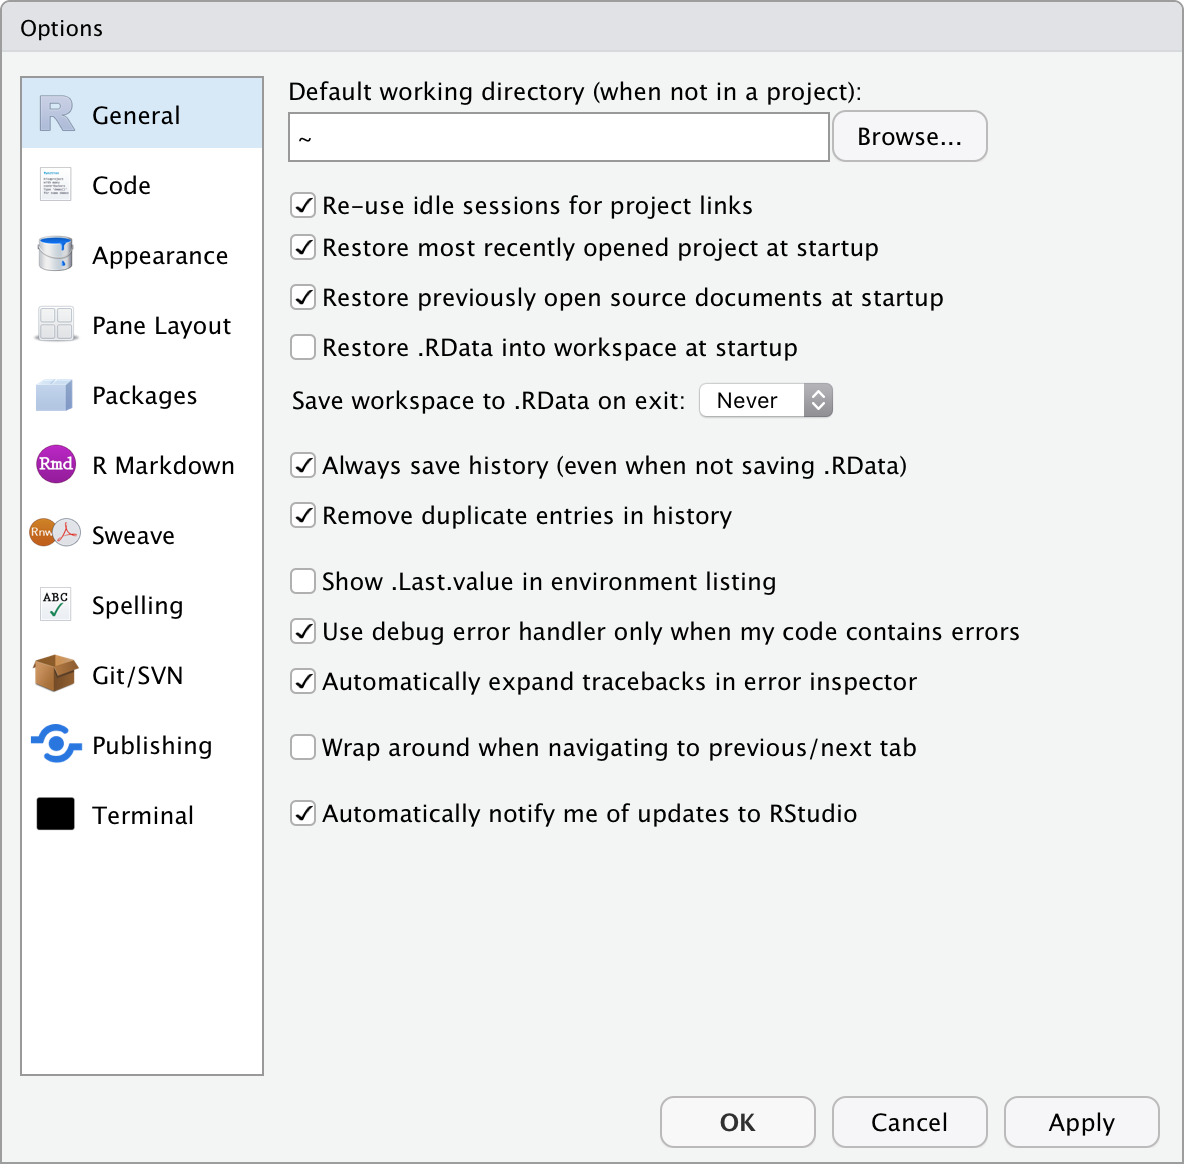
\includegraphics[width=1\linewidth]{figures/RStudio_preferences} 

}

\caption{The RStudio Preferences menu.}\label{fig:RStudio-prefs}
\end{figure}

\hypertarget{customising-appearance}{%
\subsection{Customising appearance}\label{customising-appearance}}

RStudio is highly customisable. Under the \textbf{Appearance} tab under `Tools'/`Global Options' you can see all of the different themes that come with RStudio. We recommend choosing a theme with a black background (\emph{e.g.} Chaos) as this will be easier on your eyes and your computer. It is also good to choose a theme with a sufficient amount of contrast between the different colours used to denote different types of objects/values in your code.

\hypertarget{configuring-panes}{%
\subsection{Configuring panes}\label{configuring-panes}}

You cannot rearrange panes (see below) in RStudio by dragging them, but you can alter their position via the \textbf{Pane Layout} tab in the `Tools'/`Global Options' (`RStudio'/`Preferences' -- for Mac). You may arrange the panes as you would prefer however we recommend that during the duration of this workshop you leave them in the default layout.

\hypertarget{the-rproject}{%
\section{The Rproject}\label{the-rproject}}

A very nifty way of managing workflow in RStudio is through the built-in functionality of the Rproject. We do not need to install any packages or change any settings to use these. Creating a new project is a very simple task, as well. For this course we will be using the \texttt{Intro\_R\_Workshop.Rproj} file you downloaded with the course material so that we are all running identical projects. This will prevent a lot of issues by ensuring we are doing things by the same standard. Better yet, an Rproject integrates seamlessly into version control software (\emph{e.g.} GitHub) and allows for instant world class collaboration on any research project. To initialise the `Intro\_R\_Workshop' project on your machine please find where you saved \texttt{Intro\_R\_Workshop.Rproj} file and click on it. We will cover the concepts and benefits of an Rproject more as we move through the course.

\hypertarget{installing-packages}{%
\section{Installing packages}\label{installing-packages}}

The most common functions used in R are contained within the \textbf{\texttt{base}} package; this makes R useful `out of the box.' However, there is extensive additional functionality that is being expanded all the time through the use of packages. Packages are simply collections of code called functions that automate complex mathematical or statistical tasks. One of the most useful features of R is that users are continuously developing new packages and making them available for free. You can find a comprehensive list of available packages on the \href{https://cran.r-project.org/web/packages/}{CRAN website}. There are currently (\texttt{2020-01-28}) \texttt{15363} packages available for R!

If the thought of searching for and finding R packages is daunting, a good place to start is the \href{http://cran.r-project.org/web/views/}{R Task View} page. This page curates collections of packages for general tasks you might encounter, such as Experimental Design, Meta-Analysis, or Multivariate Analysis. Go and have a look for yourself, you might be surprised to find a good explanation of what you need.

After clicking `Tools'/`Install Packages', type in the package name \textbf{\texttt{tidyverse}} in the `Packages' text box (note that it is case sensitive) and select the Install button. The \textbf{Console} will run the code needed to install the package, and then provide some commentary on the installation of the package and any of its dependencies (\emph{i.e.}, other R packages needed to run the required package).

The installation process makes sure that the functions within the packages contained within the \textbf{\texttt{tidyverse}} are now available on your computer, but to avoid potential conflicts in the names of functions, it will not load these automatically. To make R `know' about these functions in a particular session, you need either to load the package via ticking the checkbox for that package in the \textbf{Packages} tab, or execute:

\begin{Shaded}
\begin{Highlighting}[]
\KeywordTok{library}\NormalTok{(tidyverse)}
\end{Highlighting}
\end{Shaded}

To prepare ourselves for the week ahead, let us also install the following packages. Here I demonstate the command line approach to achieve the same thing that can be done via the menu:

\begin{Shaded}
\begin{Highlighting}[]
\CommentTok{\# install.packages("rmarkdown")}
\CommentTok{\# install.packages("tidyverse")}
\CommentTok{\# install.packages("bindrcpp")}
\CommentTok{\# install.packages("ggpubr")}
\CommentTok{\# install.packages("magrittr")}
\CommentTok{\# install.packages("boot")}
\CommentTok{\# install.packages("ggsn")}
\CommentTok{\# install.packages("scales")}
\CommentTok{\# install.packages("maps")}
\CommentTok{\# install.packages("ggmap")}
\CommentTok{\# install.packages("lubridate")}
\CommentTok{\# install.packages("bindrcpp")}
\end{Highlighting}
\end{Shaded}

Since we will develop the habit of doing all of our analyses from R scripts, it is best practice to simply list all of the libraries to be loaded right at the start of your script. Comments may be used to remind your future-self (to quote Hadley Wickham) what those packages are for.

\begin{quote}
\textbf{Copying code from RStudio}\\
Here you saw RStudio execute the R code needed to install (using \texttt{install.packages()}) and load (using \texttt{library()}) the package, so if you want to include these in one of your programs, just copy the text it executes. Note that you need only install the current version of a package once, but it needs to be loaded at the beginning of each R session.
\end{quote}

\begin{quote}
\textbf{Question}
Why is it best practice to include packages you use in your R program explicitly?
\end{quote}

\hypertarget{the-panes-of-rstudio}{%
\section{The panes of RStudio}\label{the-panes-of-rstudio}}

RStudio has four main panes each in a quadrant of your screen: \textbf{Source Editor}, \textbf{Console}, \textbf{Workspace Browser} (and \textbf{History}), and \textbf{Plots} (and \textbf{Files}, \textbf{Packages}, \textbf{Help}). These can also be adjusted under the `Preferences' menu. Note that there might be subtle differences between RStudio installations on different operating systems. We will discuss each of the panes in turn.

\hypertarget{source-editor}{%
\subsection{Source Editor}\label{source-editor}}

Generally we will want to write programs longer than a few lines. The \textbf{Source Editor} can help you open, edit and execute these programs. Let us open a simple program:

\begin{enumerate}
\def\labelenumi{\arabic{enumi}.}
\item
  Use Windows Explorer (Finder on Mac) and navigate to the file \texttt{BONUS/the\_new\_age.R}.
\item
  Now make RStudio the default application to open \texttt{.R} files (right click on the file Name and set RStudio to open it as the default if it isn't already)
\item
  Now double click on the file -- this will open it in RStudio in the \textbf{Source Editor} in the top left pane.
\end{enumerate}

Note \texttt{.R} files are simply standard text files and can be created in any text editor and saved with a \texttt{.R} (or \texttt{.r}) extension, but the Source editor in RStudio has the advantage of providing syntax highlighting, code completion, and smart indentation. You can see the different colours for numbers and there is also highlighting to help you count brackets (click your cursor next to a bracket and push the right arrow and you will see its partner bracket highlighted). We can execute R code directly from the Source Editor. Try the following (for Windows machines; for Macs replace \textbf{Ctrl} with \textbf{Cmd}):

\begin{itemize}
\tightlist
\item
  Execute a single line (Run icon or \textbf{Ctrl+Enter}). Note that the cursor can be anywhere on the line and one does not need to highlight anything --- do this for the code on line 2
\item
  Execute multiple lines (Highlight lines with the cursor, then Run icon or \textbf{Ctrl+Enter}) --- do this for line 3 to 6
\item
  Execute the whole script (Source icon or \textbf{Ctrl+Shift+Enter})
\end{itemize}

Now, try changing the x and/or y axis labels on line 18 and re-run the script.

Now let us save the program in the \textbf{Source Editor} by clicking on the file symbol (note that the file symbol is greyed out when the file has not been changed since it was last saved).

At this point, it might be worth thinking a bit about what the program is doing. R requires one to think about what you are doing, not simply clicking buttons like in some other software systems which shall remain nameless for now\ldots{} Scripts execute sequentially from top to bottom. Try and work out what each line of the program is doing and discuss it with your neighbour. Note, if you get stuck, try using R's help system; accessing the help system is especially easy within RStudio --- see if you can figure out how to use that too.

\begin{quote}
\textbf{Comments}\\
The hash (\texttt{\#}) tells R not to run any of the text on that line to the right of the symbol. This is the standard way of commenting R code; it is VERY good practice to comment in detail so that you can understand later what you have done.
\end{quote}

\hypertarget{console}{%
\subsection{Console}\label{console}}

This is where you can type code that executes immediately. This is also known as the command line. Throughout the notes, we will represent code for you to execute in R as a different font.

\begin{quote}
\textbf{Type it in!}
Although it may appear that one could copy code from this PDF into the \textbf{Console}, you really shouldn't. The first reason is that you might unwittingly copy invisible PDF formatting errors into R, which will make the code fail. But more importantly, typing code into the \textbf{Console} yourself gives you the practice you need, and allows you to make (and correct) your own errors. This is an invaluable way of learning and taking shortcuts now will only hurt you in the long run.
\end{quote}

Entering code in the command line is intuitive and easy. For example, we can use R as a calculator by typing into the Console (and pressing \textbf{Enter} after each line):

\begin{Shaded}
\begin{Highlighting}[]
\DecValTok{6} \OperatorTok{*}\StringTok{ }\DecValTok{3}
\end{Highlighting}
\end{Shaded}

\begin{verbatim}
R> [1] 18
\end{verbatim}

\begin{Shaded}
\begin{Highlighting}[]
\DecValTok{5} \OperatorTok{+}\StringTok{ }\DecValTok{4}
\end{Highlighting}
\end{Shaded}

\begin{verbatim}
R> [1] 9
\end{verbatim}

\begin{Shaded}
\begin{Highlighting}[]
\DecValTok{2} \OperatorTok{\^{}}\StringTok{ }\DecValTok{3}
\end{Highlighting}
\end{Shaded}

\begin{verbatim}
R> [1] 8
\end{verbatim}

Note that spaces are optional around simple calculations.

We can also use the assignment operator \texttt{\textless{}-} to assign any calculation to a variable so we can access it later (the \texttt{=} sign would work, too, but it's bad practice to use it\ldots{} and we'll talk about this as we go):

\begin{Shaded}
\begin{Highlighting}[]
\NormalTok{a <{-}}\StringTok{ }\DecValTok{2}
\NormalTok{b <{-}}\StringTok{ }\DecValTok{7}
\NormalTok{a }\OperatorTok{+}\StringTok{ }\NormalTok{b}
\end{Highlighting}
\end{Shaded}

\begin{verbatim}
R> [1] 9
\end{verbatim}

To type the assignment operator (\texttt{\textless{}-}) push the following two keys together: \textbf{alt -}. There are many keyboard shortcuts in R and we will introduce them as we go along.

Spaces are also optional around assignment operators. It is good practice to use single spaces in your R scripts, and the \textbf{alt -} shortcut will do this for you automagically. Spaces are not only there to make the code more readable to the human eye, but also to the machine. Try this:

\begin{Shaded}
\begin{Highlighting}[]
\NormalTok{d<{-}}\DecValTok{2}
\NormalTok{d }\OperatorTok{<}\StringTok{ }\DecValTok{{-}2}
\end{Highlighting}
\end{Shaded}

Note that the first line of code assigns \texttt{d} a value of \texttt{2}, whereas the second statement asks R whether this variable has a value less than 2. When asked, it responds with FALSE. If we hadn't used spaces, how would R have known what we meant?

Another important question here is, is R case sensitive? Is \texttt{A} the same as \texttt{a}? Figure out a way to check for yourself.

\hypertarget{exercise}{%
\section{Exercise}\label{exercise}}

What are the values after each statement in the following?

\begin{Shaded}
\begin{Highlighting}[]
\NormalTok{mass <{-}}\StringTok{ }\DecValTok{48} 
\NormalTok{mass <{-}}\StringTok{ }\NormalTok{mass }\OperatorTok{*}\StringTok{ }\FloatTok{2.0} \CommentTok{\# mass? }
\NormalTok{age <{-}}\StringTok{ }\NormalTok{age }\OperatorTok{{-}}\StringTok{ }\DecValTok{17} \CommentTok{\# age? m}
\NormalTok{mass\_index <{-}}\StringTok{ }\NormalTok{mass }\OperatorTok{/}\StringTok{ }\NormalTok{age }\CommentTok{\# mass\_index?}
\end{Highlighting}
\end{Shaded}

Use R to calculate some simple mathematical expressions entered.

Assign the value of 40 to \texttt{x} and Assign the value of 23 to \texttt{y}. Make \texttt{z} the value of \texttt{x-y} Display \texttt{z} in the console

We can create a vector in R by using the combine \texttt{c()} function:

\begin{Shaded}
\begin{Highlighting}[]
\NormalTok{apples <{-}}\StringTok{ }\KeywordTok{c}\NormalTok{(}\FloatTok{5.3}\NormalTok{, }\FloatTok{3.8}\NormalTok{, }\FloatTok{4.5}\NormalTok{)}
\end{Highlighting}
\end{Shaded}

A vector is a one-dimensional array (\emph{i.e.}, a list of numbers), and this is the simplest form of data used in R (you can think of a single value in R as just a very short vector). We'll talk about more complex (and therefore more powerful) types of data structures as we go along.

If you want to display the value of apples type:

\begin{Shaded}
\begin{Highlighting}[]
\NormalTok{apples}
\end{Highlighting}
\end{Shaded}

\begin{verbatim}
R> [1] 5.3 3.8 4.5
\end{verbatim}

Finally, there are default functions in R for nearly all basic statistical analyses, including \texttt{mean()} and \texttt{sd()} (standard deviation):

\begin{Shaded}
\begin{Highlighting}[]
\KeywordTok{mean}\NormalTok{(apples)}
\end{Highlighting}
\end{Shaded}

\begin{verbatim}
R> [1] 4.533333
\end{verbatim}

\begin{Shaded}
\begin{Highlighting}[]
\KeywordTok{sd}\NormalTok{(apples)}
\end{Highlighting}
\end{Shaded}

\begin{verbatim}
R> [1] 0.7505553
\end{verbatim}

\begin{quote}
\textbf{Variable names}\\
It is best not to use \texttt{c} as the name of a value or array. Why? What other words might not be good to use?
\end{quote}

Or try this:

\begin{Shaded}
\begin{Highlighting}[]
\KeywordTok{round}\NormalTok{(}\KeywordTok{sd}\NormalTok{(apples), }\DecValTok{2}\NormalTok{)}
\end{Highlighting}
\end{Shaded}

\begin{verbatim}
R> [1] 0.75
\end{verbatim}

\begin{quote}
\textbf{Question}\\
What did we do above? What can you conclude from those functions?
\end{quote}

RStudio supports the automatic completion of code using the \textbf{Tab} key. For example, type the three letters \texttt{app} and then the \textbf{Tab} key. What happens?

The code completion feature also provides brief inline help for functions whenever possible. For example, type \texttt{mean()} and press the \textbf{Tab} key.

The RStudio \textbf{Console} automagically maintains a `history' so that you can retrieve previous commands, a bit like your Internet browser or Google (\emph{see the code in: BONUS/mapping\_yourself.Rmd}). On a blank line in the \textbf{Console}, press the up arrow, and see what happens.

If you wish to review a list of your recent commands and then select a command from this list you can use \textbf{Ctrl+Up} to review the list (\textbf{Cmd+Up} on the Mac). If you prefer a `bird's eye' overview of the R command history, you may also use the RStudio History pane (see below).

The \textbf{Console} title bar has a few useful features:

\begin{enumerate}
\def\labelenumi{\arabic{enumi}.}
\item
  It displays the current R working directory (more on this later)
\item
  It provides the ability to interrupt R during a long computation (a stop sign will appear whilst code is running)
\item
  It allows you to minimise and maximise the \textbf{Console} in relation to the \textbf{Source pane} using the buttons at the top-right or by double-clicking the title bar)
\end{enumerate}

\hypertarget{environment-and-history-panes}{%
\subsection{Environment and History panes}\label{environment-and-history-panes}}

The \textbf{Environment} pane is very useful as it shows you what objects (\emph{i.e.}, dataframes, arrays, values and functions) you have in your environment (workspace). You can see the values for objects with a single value and for those that are longer R will tell you their class. When you have data in your environment that have two dimensions (rows and columns) you may click on them and they will appear in the \textbf{Source Editor} pane like a spreadsheet.

You can then go back to your program in the \textbf{Source Editor} by clicking its tab or closing the tab for the object you opened. Also in the \textbf{Environment} is the History tab, where you can see all of the code executed for the session. If you double-click a line or highlight a block of lines and then double-click those, you can send it to the \textbf{Console} (\emph{i.e.}, run them).

Typing the following into the \textbf{Console} will list everything you've loaded into the Environment:

\begin{Shaded}
\begin{Highlighting}[]
\KeywordTok{ls}\NormalTok{()}
\end{Highlighting}
\end{Shaded}

\begin{verbatim}
R> [1] "a"        "apples"   "b"        "pkgs_lst" "url"
\end{verbatim}

What do we have loaded into our environment? Did all of these objects come from one script, or more than one? How can we tell where an object was generated?

\hypertarget{files-plots-packages-help-and-viewer-panes}{%
\subsection{Files, Plots, Packages, Help, and Viewer panes}\label{files-plots-packages-help-and-viewer-panes}}

The last pane has a number of different tabs. The Files tab has a navigable file manager, just like the file system on your operating system. The \textbf{Plot} tab is where graphics you create will appear. The \textbf{Packages} tab shows you the packages that are installed and those that can be installed (more on this just now). The \textbf{Help} tab allows you to search the R documentation for help and is where the help appears when you ask for it from the \textbf{Console}.

Methods of getting help from the \textbf{Console} include\ldots{}

\begin{Shaded}
\begin{Highlighting}[]
\NormalTok{?mean}
\end{Highlighting}
\end{Shaded}

\ldots or:

\begin{Shaded}
\begin{Highlighting}[]
\KeywordTok{help}\NormalTok{(mean)}
\end{Highlighting}
\end{Shaded}

We will go into this in more detail in the next session.

To reproduced Figure \ref{fig:ggplot2-1} in the \textbf{Plot} tab, simply copy and paste the following code into the \textbf{Console}:

\begin{Shaded}
\begin{Highlighting}[]
\KeywordTok{library}\NormalTok{(tidyverse)}
\NormalTok{x <{-}}\StringTok{ }\KeywordTok{seq}\NormalTok{(}\DecValTok{0}\NormalTok{, }\DecValTok{2}\NormalTok{, }\DataTypeTok{by =} \FloatTok{0.01}\NormalTok{)}
\NormalTok{y <{-}}\StringTok{ }\DecValTok{2} \OperatorTok{*}\StringTok{ }\KeywordTok{sin}\NormalTok{(}\DecValTok{2} \OperatorTok{*}\StringTok{ }\NormalTok{pi }\OperatorTok{*}\StringTok{ }\NormalTok{(x }\OperatorTok{{-}}\StringTok{ }\DecValTok{1}\OperatorTok{/}\DecValTok{4}\NormalTok{))}
\KeywordTok{ggplot}\NormalTok{() }\OperatorTok{+}
\StringTok{  }\KeywordTok{geom\_point}\NormalTok{(}\KeywordTok{aes}\NormalTok{(}\DataTypeTok{x =}\NormalTok{ x, }\DataTypeTok{y =}\NormalTok{ y), }\DataTypeTok{shape =} \DecValTok{21}\NormalTok{, }\DataTypeTok{col =} \StringTok{"salmon"}\NormalTok{, }\DataTypeTok{fill =} \StringTok{"white"}\NormalTok{)}
\end{Highlighting}
\end{Shaded}

\begin{figure}
\centering
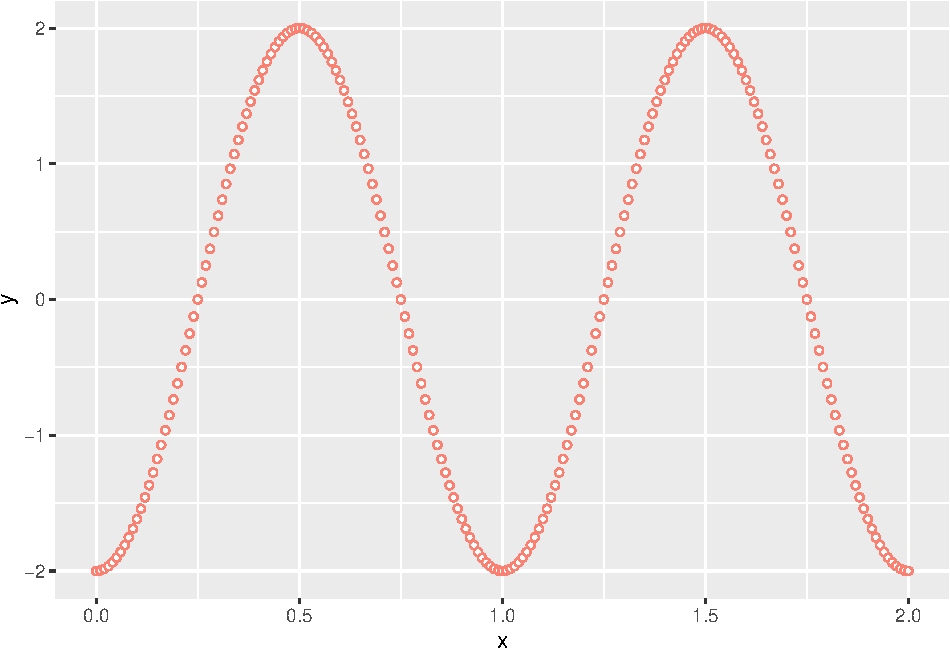
\includegraphics{02-RStudio_files/figure-latex/ggplot2-1-1.pdf}
\caption{\label{fig:ggplot2-1}The same plot as above, but assembled with \textbf{ggplot2}.}
\end{figure}

\hypertarget{session-info-1}{%
\section{Session info}\label{session-info-1}}

\begin{Shaded}
\begin{Highlighting}[]
\KeywordTok{installed.packages}\NormalTok{()[}\KeywordTok{names}\NormalTok{(}\KeywordTok{sessionInfo}\NormalTok{()}\OperatorTok{$}\NormalTok{otherPkgs), }\StringTok{"Version"}\NormalTok{]}
\end{Highlighting}
\end{Shaded}

\begin{verbatim}
R>   forcats   stringr     purrr     readr    tibble   ggplot2 tidyverse     tidyr 
R>   "0.4.0"   "1.4.0"   "0.3.3"   "1.3.1"   "2.1.3"   "3.2.1"   "1.3.0"   "1.0.0" 
R>     dplyr     rvest      xml2 
R>   "0.8.3"   "0.3.5"   "1.2.2"
\end{verbatim}

\hypertarget{github}{%
\chapter{GitHub}\label{github}}

\hypertarget{what-is-github}{%
\section{What is GitHub?}\label{what-is-github}}

GitHub is a code hosting platform for version control and collaboration. It uses the software Git to let you and others work together on projects from anywhere. The following teaches you the GitHub essentials like \textbf{Repositories}, \textbf{Branches}, \textbf{Commits}, and \textbf{Pull Requests}. You will first create your own account and repository, and learn GitHub's Pull and Push Request workflow, a popular way to create and review code.

\hypertarget{installing-git-on-windows}{%
\section{Installing Git on Windows}\label{installing-git-on-windows}}

By default, Git is installed on Linux and macOS computers as a command line option. However, Microsoft Windows does not include a Git command. To install GitHub on Windows open the Git website (\url{https://git-scm.com/}). Click the `Download' link to download Git. The download should automatically start. Once downloaded, start the installation from the browser or the download folder. In the `Select Components' window, leave all default options checked and check any other additional components you want installed. Click the `Install' button. Once completed, you can check the option to launch Git Bash if you want to open a Bash command line.

\hypertarget{create-and-account-and-a-repository}{%
\section{Create and account and a repository}\label{create-and-account-and-a-repository}}

Create a GitHub account (\url{https://github.com/join}), complete the application steps. This should take less than five minutes. Now lets create a repository. A repository is usually used to organise a single project. Repositories can contain folders and files, images, videos, spreadsheets, and data sets -- anything your project needs. We recommend including a README, or a file with information about your project. GitHub makes it easy to add one at the same time you create your new repository.

Create a new repository --- in the upper right corner, next to your avatar or identicon, click and then select `New repository'. Name your repository (Intro\_R) and write a short description.

\hypertarget{git-configuring-activation-and-connecting-to-a-remote-repository}{%
\section{Git configuring (activation) and connecting to a remote repository}\label{git-configuring-activation-and-connecting-to-a-remote-repository}}

Launch Git Bash and type the following command to configure your Git username, where will be your GitHub username:

\begin{verbatim}
        git config --global user.name "<your name>"
\end{verbatim}

After entering the above command, you should be returned to the command prompt. Next, enter your e-mail address by typing the following command, where is your e-mail address.

\begin{verbatim}
        git config --global user.email "<your e-mail>"
\end{verbatim}

\hypertarget{clone-the-new-github-repository-to-your-computer-via-rstudio.}{%
\section{Clone the new GitHub repository to your computer via RStudio.}\label{clone-the-new-github-repository-to-your-computer-via-rstudio.}}

Select the repository URL from GitHub. It will be something like \url{https://github.com/AmierohAbrahams/Intro_R}.

Enter RStudio. On the top left of the screen select the tab `New Project'. Then select the `Version control' tab followed by the `Git' tab. Complete each option by placing the repository URL into the first box and complete the rest.

\hypertarget{commits}{%
\section{Commits}\label{commits}}

Bravo! Now, on GitHub, saved changes are called \emph{Commits}. Each commit has an associated commit message, which is a description explaining why a particular change was made. Commit messages capture the history of your changes, so other contributors can understand what you've done and why.
Make and commit changes.

\hypertarget{open-a-pull-request}{%
\section{Open a Pull Request}\label{open-a-pull-request}}

Nice edits! Now that you have changes in a branch off of master, you can open a Pull Request.

Pull Requests are the heart of collaboration on GitHub. When you open a pull request, you're proposing your changes and requesting that someone review and pull in your contribution and merge them into their branch. Pull requests show diffs, or differences, of the content from both branches. The changes, additions, and subtractions are shown in green and red.

As soon as you make a commit, you can open a pull request and start a discussion, even before the code is finished.

\hypertarget{workflow}{%
\chapter{An R workflow}\label{workflow}}

\begin{quote}
``A dream doesn't become reality through magic; it takes sweat, determination and hard work.''

--- Colin Powell
\end{quote}

\begin{quote}
``Choose a job you love, and you will never have to work a day in your life.''

--- Confucius
\end{quote}

\hypertarget{r-scripts}{%
\section{R Scripts}\label{r-scripts}}

The first step for any project in R is to create a new script. We do this by clicking on the `New Document' button (in the top left and selecting `R Script'). This creates an unnamed file in the \textbf{Source Editor} pane. Best to save it first of all so we do not lose what we do. `File'/`Save As'/ and the Working Directory should come up. Type in \texttt{Day\_1} as the file name and click `save.' R will automatically add a \texttt{.R} extension.

It is recommended to start a script with some basic information for you to refer back to later. Start with a comment line (the line begins with a \texttt{\#}) that tells you the name of the script, something about the script, who created it, and the date it was created. In the source editor enter to following lines and save the file again:

\begin{Shaded}
\begin{Highlighting}[]
\CommentTok{\# Day\_1.R}
\CommentTok{\# Reads in some data about Laminaria collected along the Cape Peninsula}
\CommentTok{\# Do various data manipulations, analyses and graphs}
\CommentTok{\# <your\_name>}
\CommentTok{\# <curent\_date>}
\end{Highlighting}
\end{Shaded}

Remember that anything appearing after the \texttt{\#} is not executed by R as script and is a comment.

It is recommend that for each workshop session you start a new script (in the \textbf{Source Editor}), type in the code as we go along, and only execute the required lines. That way you will have a record of what you have done.

Below we will learn how to import the file \texttt{laminaria.csv} into R, assign it to a dataframe named \texttt{laminaria}, and spend a while looking it over. These data reflect results of a sampling campaign on one of the species of kelps (\emph{Laminaria pallida}) in the Western Cape designed to find the morphometric properties of populations at different sites. We visited 13 different locations along the Cape Peninsula (\texttt{site}), and at each site, collected \emph{ca.} 13 specimens of the largest kelps we could find. We then brought the kelps back to the shore and measured/calculated nine morphometric properties of the plants (\emph{e.g.} the mass of the fronds (\texttt{blade\_weight}), the frond length (\texttt{blade\_length}), \emph{etc.}).

\hypertarget{reading-data-into-r}{%
\section{Reading data into R}\label{reading-data-into-r}}

We will now see how easy it is to read data into R. R will read in many types of data, including spreadsheets, text files, binary files and files from other statistical packages and software.

\begin{quote}
\textbf{Full stops}\\
Unfortunately in South Africa we are taught from a young age to use commas (\texttt{,}) instead of full stops (\texttt{.}) for decimal places. This simply will not do when we are working with a computer. You must always use a full stop for a decimal place and never insert commas anywhere into any numbers.
\end{quote}

\begin{quote}
\textbf{Commas}\\
R generally thinks that commas mean the user is telling the computer to separate values. So if you think you are typing a big number like 2,300 you may actually end up with two numbers. Never use commas with numbers.
\end{quote}

\hypertarget{preparing-data-for-r}{%
\subsection{Preparing data for R}\label{preparing-data-for-r}}

Importing data can actually take longer than the statistical analysis itself! In order to avoid as much frustration as possible it is important to remember that for R to be able to analyse your data they need to be in a consistent format, with each variable in a column and each sample in a row. The format within each variable (column) needs to be consistent and is commonly one of the following types: a continuous numeric variable (\emph{e.g.}, fish length (m): \texttt{0.133}, \texttt{0.145}); a factor or categorical variable (\emph{e.g.}, Month: \texttt{Jan}, \texttt{Feb} or \texttt{1}, \texttt{2}, \texttt{\ldots{}}, \texttt{12}); a nominal variable (\emph{e.g.}, algal colour: \texttt{red}, \texttt{green}, \texttt{brown}); or a logical variable (\emph{i.e.}, \texttt{TRUE} or \texttt{FALSE}). You can also use other more specific formats such as dates and times, and more general text formats.

We will learn more about working with data in R --- specifically, we will teach you about the \emph{tidyverse} principles and the distinction between \emph{long} and \emph{wide} format data in more detail on Day 4. For most of our work in R we require our data to be in the long format, but Excel users (poor things!) are more familiar with data stored in the wide format. For now let's bring some data into R and not worry too much about the data being tidy.

\hypertarget{converting-data}{%
\subsection{Converting data}\label{converting-data}}

Before we can read in the \emph{Laminaria} dataset provided for the following exercises, we need to convert the Excel file supplied into a \texttt{.csv} file. Open `laminaria.xlsx' in Excel, then select `Save As' from the File menu. In the `Format' drop-down menu, select the option called `Comma Separated Values', then hit `Save'. You'll get a warning that formatting will be removed and that only one sheet will be exported; simply `Continue'. Your working directory should now contain a file called \texttt{laminaria.csv}.

\hypertarget{importing-data}{%
\subsection{Importing data}\label{importing-data}}

The easiest way to import data into R is by changing your working directory to be the same as the file path where the file(s) are you want to load. A file path is effectively an address. In most operating systems, if you open the folder where your files are you may click on the navigation bar and it will show you the complete file path. Many people develop the nasty habit of squirling away their files within folders within folders within folders within folders\ldots{} within folders within folders. Please don't do that.

The concept of file paths is either one that you are familiar with, or you've never heard of before. There tends to be little middle ground. Happily, RStudio allows us to circumvent this issue. We do this by using the \texttt{Intro\_R\_Workshop.Rproj} that you may find in the files downloaded for this workshop. If you have not already switched to the \texttt{Intro\_R\_Workshop.Rproj} as outlined in Chapter 2, click on the project button in the top right corner your RStudio window. Then navigate to where you saved \texttt{Intro\_R\_Workshop.Rproj} and select it. Notice that your RStudio has changed a bit and all of the objects you may have previously created in your environment have been removed and any tabs in the source editor pane have been closed. That is fine for now, but it may mean you need to re-open the \texttt{Day\_1.R} script you just created.

Once we have the working directory set, either by doing it manually with \texttt{setwd()} or by loading a project, R will now know where to look for the files we want to read. The function \texttt{read\_csv()} is the most convenient way to read in raw data. There are several other ways to read in data, but for the purposes of this workshop we'll stick to this one, for now. To find out what it does, we will go to its help entry in the usual way (\emph{i.e.} \texttt{?read\_csv}).

All R Help items are in the same format. A short \emph{Description} (of what it does), \emph{Usage}, \emph{Arguments} (the different inputs it requires), \emph{Details} (of what it does), \emph{Value} (what it returns) and \emph{Examples}. Arguments (the parameters that are passed to the function) are the lifeblood of any function, as this is how you provide information to R. You do not need to specify all arguments, as most have appropriate default values for your requirements, and others might not be needed for your particular case.

\begin{quote}
\textbf{Data formats}\\
R has pedantic requirements for naming variables. It is safest to not use spaces, special characters (\emph{e.g.}, commas, semicolons, any of the shift characters above the numbers), or function names (\emph{e.g.}, mean). One can use `camelCase', such as \texttt{myFirstVariable}, or simply separate the `parts' of the variable name using an underscore such as in \texttt{my\_first\_variable}. Always make sure to use meaningful names; eventually you will learn to find a balance between meaningfulness and something short that's easy enough to retype repeatedly (although R's ability to use tab completion helps with not having to type long names to often).
\end{quote}

\begin{quote}
\textbf{Import}\\
\texttt{read\_csv()} is simply a `wrapper' (\emph{i.e.}, a command that modifies) a more basic command called \texttt{read\_delim()}, which itself allows you to read in many types of files besides \texttt{.csv}. To find out more, type \texttt{?read\_delim()}.
\end{quote}

\hypertarget{loading-a-file}{%
\subsection{Loading a file}\label{loading-a-file}}

To load the \texttt{laminaria.csv} file we created, and assign it to an object name in R, we will use the \texttt{read\_csv()} function from the \textbf{\texttt{tidyverse}} package, so let's make sure it is activated.

\begin{Shaded}
\begin{Highlighting}[]
\KeywordTok{library}\NormalTok{(tidyverse)}
\end{Highlighting}
\end{Shaded}

Depending on the version of Excel you are using, or perhaps the settings within it, the `laminaria.csv' file you created may be corrupted in different ways. Generally Excel likes to replace the \texttt{,} between columns in our .csv files with \texttt{;}. This may seem like a triviality but sadly it is not. Lucky for use, the \textbf{\texttt{tidyverse}} knows about this problem and they have made a plan. Please open your `laminaria.csv' file and look at which character is being used to separate columns. If it is \texttt{,} then we will load the data with \texttt{read\_csv()}. If the columns are separated with \texttt{;} we will use \texttt{read\_csv2()}.

\begin{Shaded}
\begin{Highlighting}[]
\CommentTok{\# Run this if \textquotesingle{}laminaria.csv\textasciigrave{} has columns separated by \textquotesingle{},\textquotesingle{}}
\NormalTok{laminaria <{-}}\StringTok{ }\KeywordTok{read\_csv}\NormalTok{(}\StringTok{"data/laminaria.csv"}\NormalTok{)}
\CommentTok{\# Run this if \textquotesingle{}laminaria.csv\textasciigrave{} has columns separated by \textquotesingle{};\textquotesingle{}}
\NormalTok{laminaria <{-}}\StringTok{ }\KeywordTok{read\_csv2}\NormalTok{(}\StringTok{"data/laminaria.csv"}\NormalTok{)}
\end{Highlighting}
\end{Shaded}

If one clicks on the newly created \texttt{laminaria} object in the \textbf{Environment} pane it will open a new panel that shows the information as a spreadsheet. To go back to your script click the appropriate tab in the \textbf{Source Editor} pane. With these data loaded we may now perform analyses on them.

At any point when working in R, you can see exactly what objects are in memory in several ways. First, you can look at the \textbf{Environment} tab in RStudio, then \textbf{Workspace Browser}. Alternatively you can type either of the following:

\begin{Shaded}
\begin{Highlighting}[]
\KeywordTok{ls}\NormalTok{()}
\CommentTok{\# or}
\KeywordTok{objects}\NormalTok{()}
\end{Highlighting}
\end{Shaded}

You can delete an object from memory by specifying the \texttt{rm()} function with the name of the object:

\begin{Shaded}
\begin{Highlighting}[]
\KeywordTok{rm}\NormalTok{(laminaria)}
\end{Highlighting}
\end{Shaded}

This will of course delete our variable, so we will import it in again using whichever of the following two lines of code matched our Excel situation.

\begin{Shaded}
\begin{Highlighting}[]
\NormalTok{laminaria <{-}}\StringTok{ }\KeywordTok{read\_csv}\NormalTok{(}\StringTok{"data/laminaria.csv"}\NormalTok{)}
\CommentTok{\# OR}
\NormalTok{laminaria <{-}}\StringTok{ }\KeywordTok{read\_csv2}\NormalTok{(}\StringTok{"data/laminaria.csv"}\NormalTok{)}
\end{Highlighting}
\end{Shaded}

\begin{quote}
\textbf{Managing variables}\\
It is good practice to remove variables from memory that you are not using, especially if they are large.
\end{quote}

\hypertarget{working-with-data}{%
\section{Working with data}\label{working-with-data}}

\hypertarget{examine-your-data}{%
\subsection{Examine your data}\label{examine-your-data}}

Once the data are in R, you need to check there are no glaring errors. It is useful to call up the first few lines of the dataframe using the function \texttt{head()}. Try it yourself by typing:

\begin{Shaded}
\begin{Highlighting}[]
\KeywordTok{head}\NormalTok{(laminaria)}
\end{Highlighting}
\end{Shaded}

This lists the first six lines of each of the variables in the dataframe as a table. You can similarly retrieve the last six lines of a dataframe by an identical call to the function \texttt{tail()}. Of course, this works better when you have fewer than 10 or so variables (columns); for larger data sets, things can get a little messy. If you want more or fewer rows in your head or tail, tell R how many rows it is you want by adding this information to your function call. Try typing:

\begin{Shaded}
\begin{Highlighting}[]
\KeywordTok{head}\NormalTok{(laminaria, }\DataTypeTok{n =} \DecValTok{3}\NormalTok{)}
\KeywordTok{tail}\NormalTok{(laminaria, }\DataTypeTok{n =} \DecValTok{2}\NormalTok{)}
\end{Highlighting}
\end{Shaded}

You can also check the structure of your data by using the \texttt{glimpse()} function:

\begin{Shaded}
\begin{Highlighting}[]
\KeywordTok{glimpse}\NormalTok{(laminaria)}
\end{Highlighting}
\end{Shaded}

This very handy function lists the variables in your dataframe by name, tells you what sorts of data are contained in each variable (\emph{e.g.}, continuous number, discrete factor) and provides an indication of the actual contents of each.

If we wanted only the names of the variables (columns) in the dataframe, we could use:

\begin{Shaded}
\begin{Highlighting}[]
\KeywordTok{names}\NormalTok{(laminaria)}
\end{Highlighting}
\end{Shaded}

\hypertarget{tidyverse-sneak-peek}{%
\subsection{Tidyverse sneak peek}\label{tidyverse-sneak-peek}}

Before we begin to manipulate our data further we need to briefly introduce ourselves to the \textbf{\texttt{tidyverse}}. And no introduction can be complete within learning about the \emph{pipe} command, \texttt{\%\textgreater{}\%}. We may type this by pushing the following keys together: \textbf{ctrl-shift-m}. The pipe (\texttt{\%\textgreater{}\%}) allows us to perform calculations sequentially, which helps us to avoid making errors.

The pipe works best in tandem with the following five common functions:

\begin{itemize}
\tightlist
\item
  Arrange observations (rows) with \texttt{arrange()}\\
\item
  Filter observations (rows) with \texttt{filter()}\\
\item
  Select variables (columns) with\texttt{select()}\\
\item
  Create new variables (columns) with \texttt{mutate()}\\
\item
  Summarise variables (columns) with \texttt{summarise()}
\end{itemize}

We will cover these functions in more detail on Day 4. For now we will ease ourselves into the code with some simple examples.

\hypertarget{subsetting}{%
\subsection{Subsetting}\label{subsetting}}

Now let's have a look at specific parts of the data. You will likely need to do this in almost every script you write. If we want to refer to a variable, we specify the dataframe then the column name within the \texttt{select()} function. In your script type:

\begin{Shaded}
\begin{Highlighting}[]
\NormalTok{laminaria }\OperatorTok{\%>\%}\StringTok{ }\CommentTok{\# Tell R which dataframe we are using}
\StringTok{  }\KeywordTok{select}\NormalTok{(site, total\_length) }\CommentTok{\# Select only specific columns}
\end{Highlighting}
\end{Shaded}

If we want to only select values from specific columns we insert one more line of code.

\begin{Shaded}
\begin{Highlighting}[]
\NormalTok{laminaria }\OperatorTok{\%>\%}\StringTok{ }
\StringTok{  }\KeywordTok{select}\NormalTok{(site, total\_length) }\OperatorTok{\%>\%}\StringTok{ }\CommentTok{\# Select specific columns first}
\StringTok{  }\KeywordTok{slice}\NormalTok{(}\DecValTok{56}\OperatorTok{:}\DecValTok{78}\NormalTok{)}
\CommentTok{\# what does the \textquotesingle{}56:78\textquotesingle{} do? Change some numbers and run the code again. What happens?}
\end{Highlighting}
\end{Shaded}

If we wanted to select only the rows of data belonging to the Kommetjie site, we could type:

\begin{Shaded}
\begin{Highlighting}[]
\NormalTok{laminaria }\OperatorTok{\%>\%}
\StringTok{  }\KeywordTok{filter}\NormalTok{(site }\OperatorTok{==}\StringTok{ "Kommetjie"}\NormalTok{)}
\end{Highlighting}
\end{Shaded}

The function \texttt{filter()} has two arguments: the first is a dataframe (we specify \texttt{laminaria} in the previous line and the pipe supplies this for us) and the second is an expression that relates to which rows of a particular variable we want to include. Here we include all rows for Kommetjie and we find that in the variable site. It returns a subset that is actually a dataframe itself; it is in the same form as the original dataframe. We could assign that subset of the full dataframe to a new dataframe if we wanted to.

\begin{Shaded}
\begin{Highlighting}[]
\NormalTok{lam\_kom <{-}}\StringTok{ }\NormalTok{laminaria }\OperatorTok{\%>\%}\StringTok{ }
\StringTok{  }\KeywordTok{filter}\NormalTok{(site }\OperatorTok{==}\StringTok{ "Kommetjie"}\NormalTok{)}
\end{Highlighting}
\end{Shaded}

\begin{quote}
\textbf{DIY: Subsetting}\\
In the script you have started, create a new named dataframe containing only kelps from two of the sites. Check that the new dataframe has the correct values in it. What purpose can the naming of a newly-created dataframe serve?
\end{quote}

\hypertarget{basic-stats}{%
\subsection{Basic stats}\label{basic-stats}}

Straight out of the box it is possible in R to perform a broad range of statistical calculations on a dataframe. If we wanted to know how many samples we have at Kommetjie, we simply type the following:

\begin{Shaded}
\begin{Highlighting}[]
\NormalTok{laminaria }\OperatorTok{\%>\%}\StringTok{ }\CommentTok{\# Tell R which dataset to use}
\StringTok{  }\KeywordTok{filter}\NormalTok{(site }\OperatorTok{==}\StringTok{ "Kommetjie"}\NormalTok{) }\OperatorTok{\%>\%}\StringTok{ }\CommentTok{\# Filter out only records from Kommetjie}
\StringTok{  }\KeywordTok{nrow}\NormalTok{() }\CommentTok{\# Count the number of remaining rows}
\end{Highlighting}
\end{Shaded}

Or, if we want to select only the row with the greatest total length:

\begin{Shaded}
\begin{Highlighting}[]
\NormalTok{laminaria }\OperatorTok{\%>\%}\StringTok{ }\CommentTok{\# Tell R which dataset to use}
\StringTok{  }\KeywordTok{filter}\NormalTok{(total\_length }\OperatorTok{==}\StringTok{ }\KeywordTok{max}\NormalTok{(total\_length)) }\CommentTok{\# Select row with max total length}
\end{Highlighting}
\end{Shaded}

\hypertarget{exercise-1}{%
\section{Exercise}\label{exercise-1}}

Using pipes, subset the laminaria data to include regions where the blade thickness is thicker than 5 cm and retain only the columns site, region, blade weight and blade thickness.

Now exit RStudio. Pretend it is three days later and revisit your analysis. Calculate the number of entries at Kommetjie and find the row with the greatest length. Do this now.

Imagine doing this daily as our analysis grows in complexity. It will very soon become quite repetitive if each day you had to retype all these lines of code. And now, six weeks into the research and attendant statistical analysis, you discover that there were some mistakes and some of the raw data were incorrect. Now everything would have to be repeated by retyping it at the command prompt. Or worse still (and bad for repetitive strain injury) doing all of it in SPSS and remembering which buttons to click and then re-clicking them. A pain. Let's avoid that altogether and do it the right way by writing an R script to automate and annotate all of this.

\begin{quote}
\textbf{Dealing with missing data}\\
The \texttt{.csv} file format is usually the most robust for reading data into R. Where you have missing data (blanks), the \texttt{.csv} format separates these by commas. However, there can be problems with blanks if you read in a space-delimited format file. If you are having trouble reading in missing data as blanks, try replacing them in your spreadsheet with \texttt{NA}, the missing data code in R. In Excel, highlight the area of the spreadsheet that includes all the cells you need to fill with \texttt{NA}. Do an Edit/Replace\ldots{} and leave the `Find what:' textbox blank and in the `Replace with:' textbox enter \texttt{NA}, the missing value code. Once imported into R, the \texttt{NA} values will be recognised as missing data.
\end{quote}

So far we have calculated the mean and standard deviation of some data in the \emph{Laminaria} data set. If you have not, please append those lines of code to the end of your script. You can run individual lines of code by highlighting them and pressing \textbf{ctrl-Enter} (\textbf{cmd-Enter} on a Mac). Do this.

Your file will now look similar to this one, but of course you will have added your own notes and comments as you went along:

\begin{Shaded}
\begin{Highlighting}[]
\CommentTok{\# Day\_1.R}
\CommentTok{\# Reads in some data about Laminaria collected along the Cape Peninsula}
\CommentTok{\# do various data manipulations, analyses and graphs}
\CommentTok{\# AJ Smit}
\CommentTok{\# 9 January 2020}

\CommentTok{\# Find the current working directory (it will be correct if a project was}
\CommentTok{\# created as instructed earlier)}
\KeywordTok{getwd}\NormalTok{()}

\CommentTok{\# If the directory is wrong because you chose not to use an Rworkspace (project),}
\CommentTok{\# set your directory manually to where the script will be saved and where the data}
\CommentTok{\# are located}
\CommentTok{\# setwd("<insert\_path\_here>")}

\CommentTok{\# Load libraries}
\KeywordTok{library}\NormalTok{(tidyverse)}

\CommentTok{\# Load the data}
\NormalTok{laminaria <{-}}\StringTok{ }\KeywordTok{read\_csv}\NormalTok{(}\StringTok{"data/laminaria.csv"}\NormalTok{)}

\CommentTok{\# Examine the data}
\KeywordTok{head}\NormalTok{(laminaria, }\DecValTok{5}\NormalTok{) }\CommentTok{\# First five lines}
\KeywordTok{tail}\NormalTok{(laminaria, }\DecValTok{2}\NormalTok{) }\CommentTok{\# Last two lines}
\KeywordTok{glimpse}\NormalTok{(laminaria) }\CommentTok{\# A more thorough summary}
\KeywordTok{names}\NormalTok{(laminaria) }\CommentTok{\# THe names of the columns}

\CommentTok{\# Subsetting data}
\NormalTok{laminaria }\OperatorTok{\%>\%}\StringTok{ }\CommentTok{\# Tell R which dataframe to use}
\StringTok{  }\KeywordTok{select}\NormalTok{(site, total\_length) }\OperatorTok{\%>\%}\StringTok{ }\CommentTok{\# Select specific columns}
\StringTok{  }\KeywordTok{slice}\NormalTok{(}\DecValTok{56}\OperatorTok{:}\DecValTok{78}\NormalTok{) }\CommentTok{\# Select specific rows}

\CommentTok{\# How many data points do we have at Kommetjie?}
\NormalTok{laminaria }\OperatorTok{\%>\%}
\StringTok{  }\KeywordTok{filter}\NormalTok{(site }\OperatorTok{==}\StringTok{ "Kommetjie"}\NormalTok{) }\OperatorTok{\%>\%}
\StringTok{  }\KeywordTok{nrow}\NormalTok{()}

\CommentTok{\# The row with the greatest length}
\NormalTok{laminaria }\OperatorTok{\%>\%}\StringTok{ }\CommentTok{\# Tell R which dataset to use}
\StringTok{  }\KeywordTok{filter}\NormalTok{(total\_length }\OperatorTok{==}\StringTok{ }\KeywordTok{max}\NormalTok{(total\_length)) }\CommentTok{\# Select row with max total length}
\end{Highlighting}
\end{Shaded}

Making sure all the latest edits in your R script have been saved, close your R session. Pretend this is now 2019 and you need to revisit the analysis. Open the file you created in 2017 in RStudio. All you need to do now is highlight the file's entire contents and hit \textbf{ctrl-Enter}.

\begin{quote}
\textbf{Stick with \texttt{.csv} files}\\
There are packages in R to read in Excel spreadsheets (\emph{e.g.}, .xlsx), but remember there are likely to be problems reading in formulae, graphs, macros and multiple worksheets. We recommend exporting data deliberately to \texttt{.csv} files (which are also commonly used in other programs). This not only avoids complications, but also allows you to unambiguously identify the data you based your analysis on. This last statement should give you the hint that it is good practice to name your \texttt{.csv} slightly differently each time you export it from Excel, perhaps by appending a reference to the date it was exported.
\end{quote}

\begin{quote}
\textbf{Remember\ldots{}}\\
Friends don't let friends use Excel.
\end{quote}

\hypertarget{summary-of-all-variables-in-a-dataframe}{%
\subsection{Summary of all variables in a dataframe}\label{summary-of-all-variables-in-a-dataframe}}

Import the data into a dataframe called \texttt{laminaria} once more (if it isn't already in your \textbf{Environment}), and check that it is in order. Once we're happy that the data have imported correctly, and that we know what the variables are called and what sorts of data they contain, we can dig a little deeper. Try typing:

\begin{Shaded}
\begin{Highlighting}[]
\KeywordTok{summary}\NormalTok{(laminaria)}
\end{Highlighting}
\end{Shaded}

The output is quite informative. It tabulates variables by name, and for each provides summary statistics. For continuous variables, the name, minimum, maximum, first, second (median) and third quartiles, and the mean are provided. For factors (categorical variables), a list of the levels of the factor and the count of each level are given. In either case, the last line of the table indicates how many NAs are contained in the variable. The function \texttt{summary()} is useful to remember as it can be applied to many different R objects (\emph{e.g.}, variables, dataframes, models, arrays, \emph{etc.}) and will give you a summary of that object. We will use it liberally throughout the workshop.

\hypertarget{summary-statistics-by-variable}{%
\subsection{Summary statistics by variable}\label{summary-statistics-by-variable}}

This is all very convenient, but we may want to ask R specifically for just the mean of a particular variable. In this case, we simply need to tell R which summary statistic we are interested in, and to specify the variable to apply it to using \texttt{summarise()}. Try typing:

\begin{Shaded}
\begin{Highlighting}[]
\NormalTok{laminaria }\OperatorTok{\%>\%}\StringTok{ }\CommentTok{\# Chose the dataframe}
\StringTok{  }\KeywordTok{summarise}\NormalTok{(}\DataTypeTok{avg\_bld\_wdt =} \KeywordTok{mean}\NormalTok{(blade\_length)) }\CommentTok{\# Calculate mean blade length}
\end{Highlighting}
\end{Shaded}

Or, if we wanted to know the mean and standard deviation for the total lengths of all the plants across all sites, do:

\begin{Shaded}
\begin{Highlighting}[]
\NormalTok{laminaria }\OperatorTok{\%>\%}\StringTok{ }\CommentTok{\# Tell R that we want to use the \textquotesingle{}laminaria\textquotesingle{} dataframe}
\StringTok{  }\KeywordTok{summarise}\NormalTok{(}\DataTypeTok{avg\_stp\_ln =} \KeywordTok{mean}\NormalTok{(total\_length), }\CommentTok{\# Create a summary of the mean of the total lengths}
            \DataTypeTok{sd\_stp\_ln =} \KeywordTok{sd}\NormalTok{(total\_length)) }\CommentTok{\# Create a summary of the sd of the total lengths}
\end{Highlighting}
\end{Shaded}

Of course, the mean and standard deviation are not the only summary statistic that R can calculate. Try \texttt{max()}, \texttt{min()}, \texttt{median()}, \texttt{range()}, \texttt{sd()} and \texttt{var()}. Do they return the values you expected? Now try:

\begin{Shaded}
\begin{Highlighting}[]
\NormalTok{laminaria }\OperatorTok{\%>\%}\StringTok{ }
\StringTok{  }\KeywordTok{summarise}\NormalTok{(}\DataTypeTok{avg\_stp\_ms =} \KeywordTok{mean}\NormalTok{(stipe\_mass))}
\end{Highlighting}
\end{Shaded}

The answer probably isn't what you would expect. Why not? Sometimes, you need to tell R how you want it to deal with missing data. In this case, you have NAs in the named variable, and R takes the cautious approach of giving you the answer of \texttt{NA}, meaning that there are missing values here. This may not seem useful, but as the programmer, you can tell R to respond differently, and it will. Simply append an argument to your function call, and you will get a different response. Type:

\begin{Shaded}
\begin{Highlighting}[]
\NormalTok{laminaria }\OperatorTok{\%>\%}\StringTok{ }
\StringTok{  }\KeywordTok{summarise}\NormalTok{(}\DataTypeTok{avg\_stp\_ms =} \KeywordTok{mean}\NormalTok{(stipe\_mass, }\DataTypeTok{na.rm =}\NormalTok{ T))}
\end{Highlighting}
\end{Shaded}

The \texttt{na.rm} argument tells R to remove (or more correctly `strip') NAs from the data string before calculating the mean. It now returns the correct answer. Although needing to deal explicitly with missing values in this way can be a bit painful, it does make you more aware of missing data, what the analyses in R are doing, and makes you decide explicitly how you will treat missing data.

\hypertarget{more-complex-calculations}{%
\subsection{More complex calculations}\label{more-complex-calculations}}

Let's say you want to calculate something that is not standard in R, say the standard error of the mean for a variable, rather than just the corresponding standard deviation. How can this be done?

The trick is to remember that R is a calculator, so we can use it to do maths, even complex maths (which we won't do). The formula for standard error is:

\[se = \sqrt{\frac{var}{n}}\]

We know that the variance is given by \texttt{var()}, so all we need to do is figure out how to get \texttt{n} and calculate a square root. The simplest way to determine the number of elements in a variable is a call to the function \texttt{nrow()}, as we saw previously. We may therefore calculate standard error with one chunk of code, step by step, using the pipe. Furthermore, by using \texttt{group\_by()} we may calculate the standard error for all sites in one go.

\begin{Shaded}
\begin{Highlighting}[]
\NormalTok{laminaria }\OperatorTok{\%>\%}\StringTok{ }\CommentTok{\# Select \textquotesingle{}laminaria\textquotesingle{}}
\StringTok{  }\KeywordTok{group\_by}\NormalTok{(site) }\OperatorTok{\%>\%}\StringTok{ }\CommentTok{\# Group the dataframe by site}
\StringTok{  }\KeywordTok{summarise}\NormalTok{(}\DataTypeTok{var\_bl =} \KeywordTok{var}\NormalTok{(blade\_length), }\CommentTok{\# Calculate variance}
            \DataTypeTok{n\_bl =} \KeywordTok{n}\NormalTok{()) }\OperatorTok{\%>\%}\StringTok{  }\CommentTok{\# Count number of values}
\StringTok{  }\KeywordTok{mutate}\NormalTok{(}\DataTypeTok{se\_bl =} \KeywordTok{sqrt}\NormalTok{(var\_bl }\OperatorTok{/}\StringTok{ }\NormalTok{n\_bl)) }\CommentTok{\# Calculate se}
\end{Highlighting}
\end{Shaded}

When calculating the mean, we specified that R should strip the NAs, using the argument \texttt{na.rm\ =\ TRUE}. In the example above, we didn't have NAs in the variable of interest. What happens if we \emph{do}?

Unfortunately, the call to the function \texttt{nrow()} has no arguments telling R how to treat NAs; instead, they are simply treated as elements of the variable and are therefore counted. The easiest way to resolve this problem is to strip out NAs in advance of any calculations. Try typing:

\begin{Shaded}
\begin{Highlighting}[]
\NormalTok{laminaria }\OperatorTok{\%>\%}\StringTok{ }
\StringTok{  }\KeywordTok{select}\NormalTok{(stipe\_mass) }\OperatorTok{\%>\%}\StringTok{ }
\StringTok{  }\KeywordTok{summarise}\NormalTok{(}\DataTypeTok{n =} \KeywordTok{n}\NormalTok{())}
\end{Highlighting}
\end{Shaded}

then:

\begin{Shaded}
\begin{Highlighting}[]
\NormalTok{laminaria }\OperatorTok{\%>\%}\StringTok{ }
\StringTok{  }\KeywordTok{select}\NormalTok{(stipe\_mass) }\OperatorTok{\%>\%}\StringTok{ }
\StringTok{  }\KeywordTok{na.omit}\NormalTok{() }\OperatorTok{\%>\%}\StringTok{ }
\StringTok{  }\KeywordTok{summarise}\NormalTok{(}\DataTypeTok{n =} \KeywordTok{n}\NormalTok{())}
\end{Highlighting}
\end{Shaded}

You will notice that the function \texttt{na.omit()} removes NAs from the variable that is specified as its argument.

\begin{quote}
\textbf{DIY: Using \texttt{na.omit()}}
Using this new information, \emph{calculate} the mean stipe mass and the corresponding standard error.
\end{quote}

\hypertarget{exercise-2}{%
\section{Exercise}\label{exercise-2}}

Create a new data frame from the laminaria dataset that meets the following criteria: contains only the site column and a new column called total\_length\_half containing values that are half of the total\_length. In this total\_length\_half column, there are no NAs and all values are less than 100. Hint: think about how the commands should be ordered to produce this data frame!

Use \texttt{group\_by()} and \texttt{summarise()} to find the mean, min, and max blade\_length for each site. Also add the number of observations (hint: see \texttt{?n}).

What was the heaviest stipe measured in each site? Return the columns \texttt{site}, \texttt{region}, and \texttt{stipe\_length}.

\hypertarget{saving-data}{%
\section{Saving data}\label{saving-data}}

A major advantage of R over many other statistics packages is that you can generate exactly the same answers time and time again by simply re-running saved code. However, there are times when you will want to output data to a file that can be read by a spreadsheet program such as Excel (but try not to\ldots{} please). The simplest general format is .csv (comma-separated values). This format is easily read by Excel, and also by many other software programs. To output a .csv type:

\begin{Shaded}
\begin{Highlighting}[]
\KeywordTok{write\_csv}\NormalTok{(site\_by\_region, }\DataTypeTok{path =} \StringTok{"data/kelp\_summary.csv"}\NormalTok{)}
\end{Highlighting}
\end{Shaded}

The first argument is simply the name of an object in R, in this case our table (a data object of class \emph{table}) of counts by region and site (other sorts of data are available, so play around to see what can be done). The second argument is the name of the file you want to write to. This file will always be written to your working directory, unless otherwise specified by including a different path in the file name. Remember that file names need to be within quotation marks. The resultant file can sadly be opened in Excel.

\hypertarget{visualisations}{%
\section{Visualisations}\label{visualisations}}

R has powerful and flexible graphics capabilities. In this Workshop we will not use the traditional graphics (\emph{i.e.} \emph{base graphics} in the graphics package automatically loaded in R). We will instead use a package called \textbf{\texttt{ggplot2}} that has the ability for extensive customisation (see the examples at the beginning of tomorrow's section), so it will cover most of the graphs that you will want to produce. We will spend the next two days working on our \textbf{\texttt{ggplot2}} skills. Here is a quick example of a \textbf{\texttt{ggplot2}} graphic made from two of the kelp variables to show the relationship between them:

\begin{Shaded}
\begin{Highlighting}[]
\KeywordTok{ggplot}\NormalTok{(}\DataTypeTok{data =}\NormalTok{ laminaria, }\KeywordTok{aes}\NormalTok{(}\DataTypeTok{x =}\NormalTok{ stipe\_mass, }\DataTypeTok{y =}\NormalTok{ stipe\_length)) }\OperatorTok{+}
\StringTok{  }\KeywordTok{geom\_point}\NormalTok{(}\DataTypeTok{shape =} \DecValTok{21}\NormalTok{, }\DataTypeTok{colour =} \StringTok{"salmon"}\NormalTok{, }\DataTypeTok{fill =} \StringTok{"white"}\NormalTok{) }\OperatorTok{+}
\StringTok{  }\KeywordTok{labs}\NormalTok{(}\DataTypeTok{x =} \StringTok{"Stipe mass (kg)"}\NormalTok{, }\DataTypeTok{y =} \StringTok{"Stipe length (cm)"}\NormalTok{)}
\end{Highlighting}
\end{Shaded}

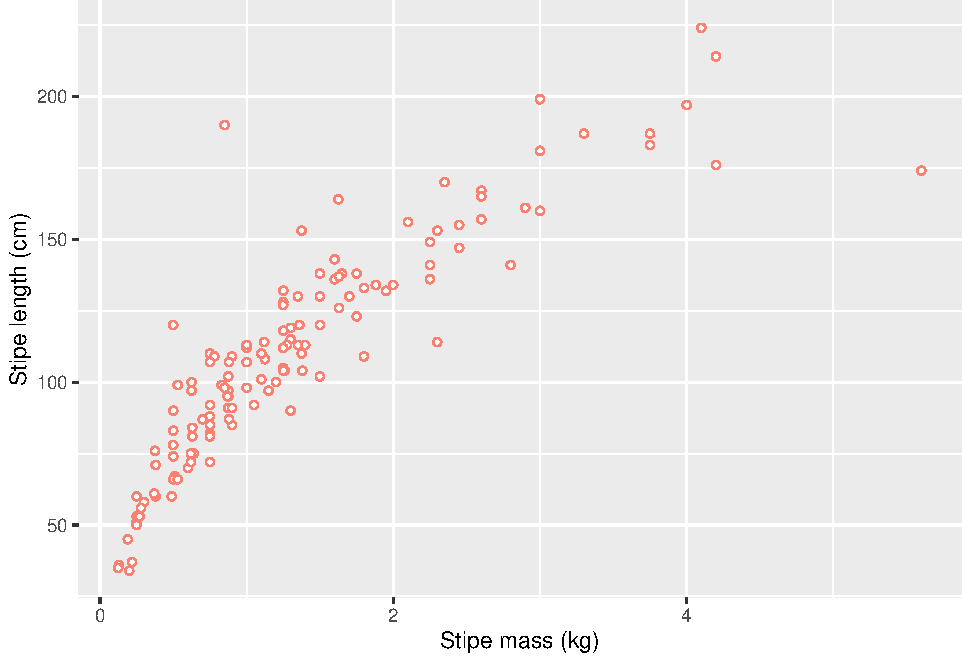
\includegraphics{04-workflow_files/figure-latex/workflow-1-1.pdf}

\hypertarget{clearing-the-memory}{%
\section{Clearing the memory}\label{clearing-the-memory}}

You will be left with many objects after working through these examples. Note that in RStudio when you quit it can save the Environment if you choose, and so it can retain the objects in memory when you start RStudio again. The choice to save the objects resulting from an R Session until next time can be selected in the Global Options menu (`Tools' \textgreater{} `Global Options' \textgreater{} `General' \textgreater{} `Save workspace to .RData on exit'). Personally, we never save objects as it is preferable to start on a clean slate when one opens RStudio. Either way, to avoid long load times and clogged memory, it is good practice to clear the objects in memory every now and then unless you can think of a compelling reason not to. This may be done by clicking on the broom icon at the top of the \textbf{Environment} pane.

Of course, you could remove an individual object by placing only its name within the brackets of \texttt{rm()}. Do not use this line of code carelessly in the middle of your script; doing so will mean that you have to go back and regenerate the objects you accidentally removed -- this is more of a nuisance than a train smash, especially for long, complicated scripts, as you will have (I hope!) saved the R script from which the objects in memory can be regenerated at any time.

\hypertarget{working-directories}{%
\section{Working directories}\label{working-directories}}

At the beginning of this session we glossed over this topic by setting the working directory via RStudio's project functionality. This concept is however critically important to understand so we must now cover it in more detail. The current working directory, where R will read and write files, is displayed by RStudio within the title region of the Console. There are a number of ways to change the current working directory:

\begin{enumerate}
\def\labelenumi{\arabic{enumi}.}
\item
  Select `Session'/`Set Working Directory' and then choose from the four options for how to set your working directory depending on your preference
\item
  From within the \textbf{Files} pane, navigate to the directory you want to set as the working directory and then select `More'/`Set As Working Directory' menu item (navigation within the Files pane alone will not change the working directory)
\item
  Use \texttt{setwd()}, providing the name of your desired working directory as a character string
\end{enumerate}

In the \textbf{Files} tab, use the directory structure to navigate to the Intro R Workshop directory\ldots{} this will differ from person to person. Then under `More', select the small upside down (drill-down) triangle and select `Set As Working Directory'. This means that whenever you read or write a file it will always be working in that directory. This gives us the code for setting the directory (below is the code that I would enter in the \textbf{Console} on my computer):

\begin{Shaded}
\begin{Highlighting}[]
\KeywordTok{setwd}\NormalTok{(}\StringTok{"\textasciitilde{}/Intro\_R\_Workshop"}\NormalTok{)}
\end{Highlighting}
\end{Shaded}

It will be different for you, but copy it into your script and make a note for future reference.

\begin{quote}
\textbf{Working directories}\\
For Windows users, if you copy from a file path the slashes will be the wrong way around and must be changed!
\end{quote}

You can check that R got this right by typing into the \textbf{Console}:

\begin{Shaded}
\begin{Highlighting}[]
\KeywordTok{getwd}\NormalTok{()}
\end{Highlighting}
\end{Shaded}

\begin{quote}
\textbf{Organising R projects}\\
For every R project, set up a separate directory that includes the scripts, data files and outputs.
\end{quote}

\hypertarget{help}{%
\section{Help}\label{help}}

The help files in R are not readily clear. It requires a bit of work to understand them well. There is method however to what appears to be madness. The figure below shows the beginning of a help file for a function in R. Please type \texttt{?read.table()} in your console now to bring up this help file in your RStudio GUI.

\begin{figure}

{\centering 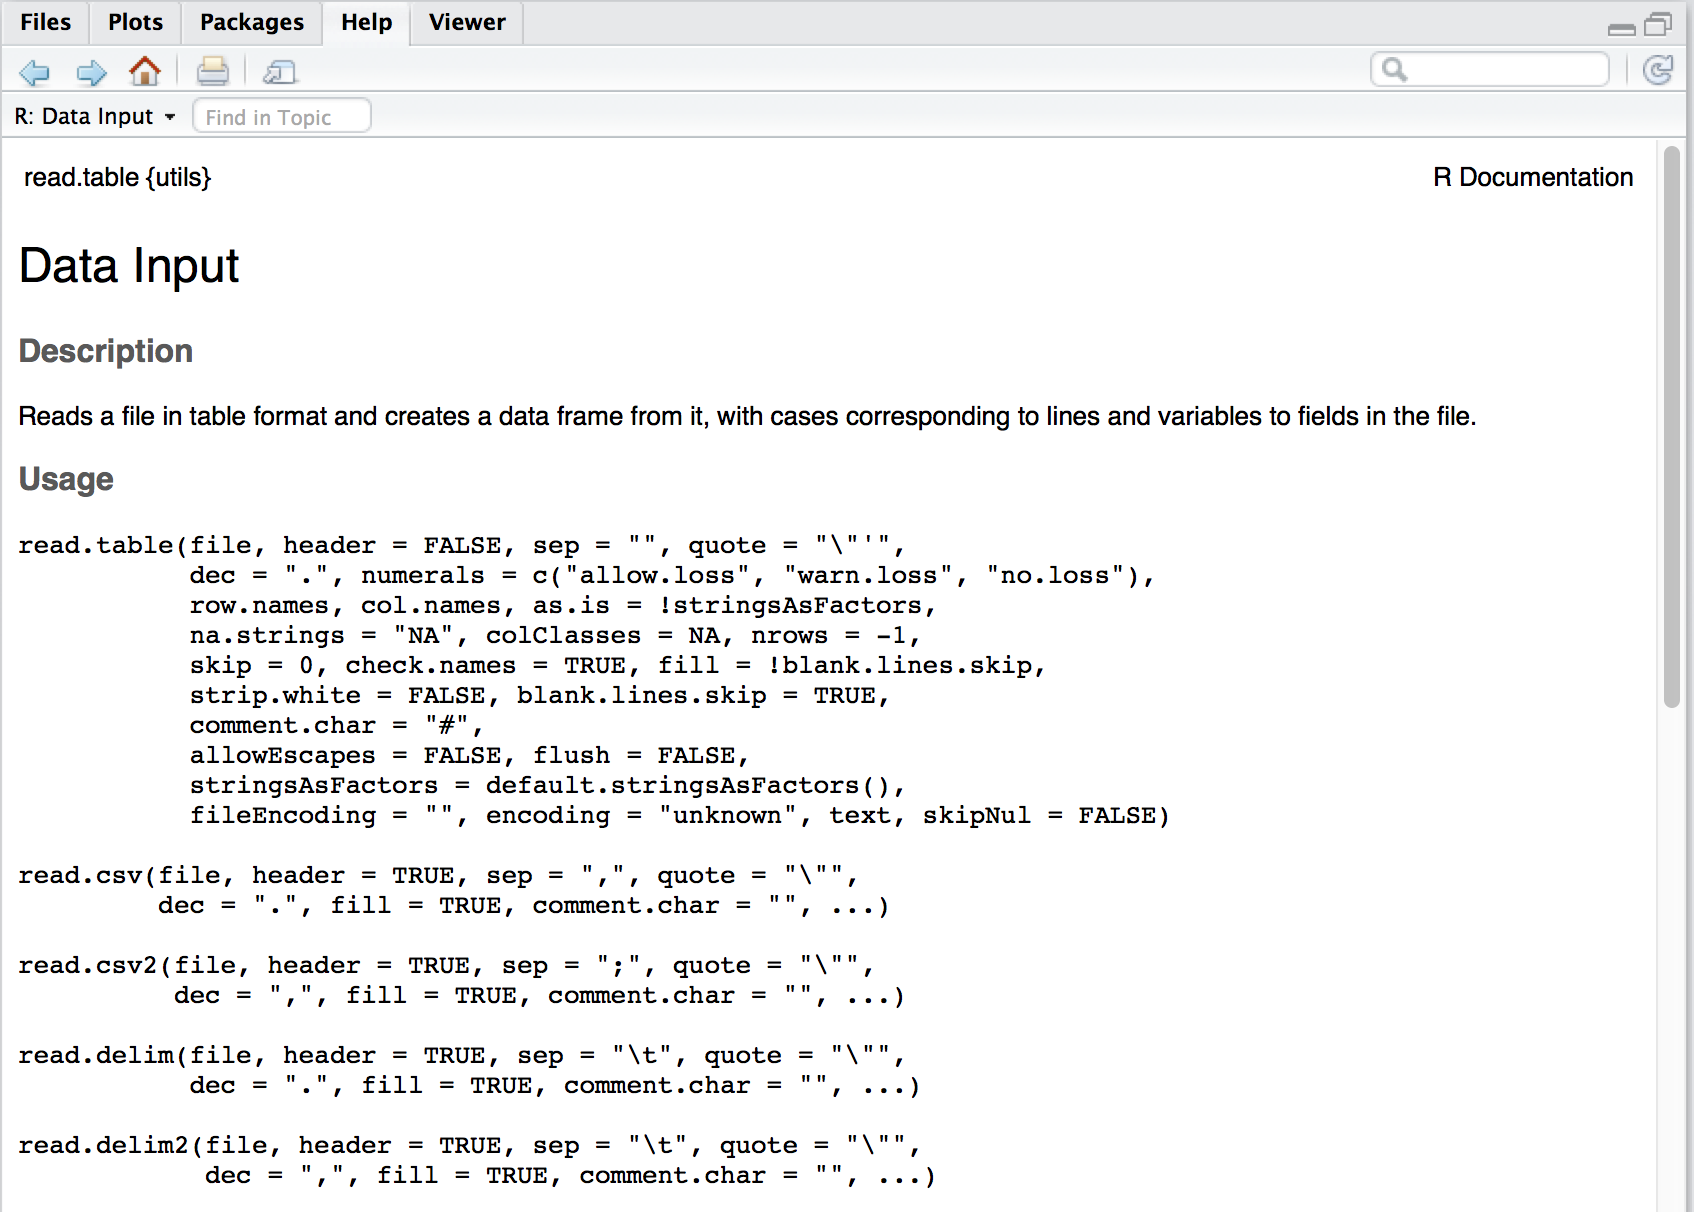
\includegraphics[width=1\linewidth]{figures/help_output} 

}

\caption{A portion of the help page produced by the above command.}\label{fig:help-output}
\end{figure}

The first thing we see at the top of the help file in small font is the name of the function, and the package it comes from in curly braces. After this, in very large text, is a very short description of what the function is used for. After this is the `Description' section, which gives a sentence or two more fully explaining the use(s) of the function. The `Usage' then shows all of the arguments that may be given to the function, and what their default settings are. When we write a function in our script we do \emph{not} need to include all of the possible arguments. The help file shows us all of them so that we know what our options are. In some cases a help file will show the usage of several different functions together. This is done, as is the case here, if these functions forma a sort of `family' and share many common purposes. The `Arguments' section gives a long explanation for what each individual argument may do. The Arguments section here is particularly verbose. Up next is the `Details' section that gives a more in depth description of what the function does. The `Value' section tells us what sort of output we may expect from the function. Some of the more well documented functions, such as this one, will have additional sections that are not a requirement for function documentation. In this case the `Memory usage' and `Note' sections are not things one should always expect to see in help files. Also not always present is a `References' section. Should there be actual published documentation for the function, or the function has been used in a publication for some other purpose, these references tend to be listed here. There are many functions in the \textbf{\texttt{vegan}} package that have been used in dozens of publications. If there is additional reading relevant to the function in question, the authors may also have included a `See also' section, but this is not standard. Lastly, any well documented function should end with an `Examples' section. The code is this section is designed to be able to be copy-pasted directly from the help file into the users R script or console and run \emph{as is}. It is perhaps a bad habit, but when I am looking up a help file for a function, I tend to look first at the Examples section. And only if I can't solve my problem with the examples do I actually read the documentation.

\hypertarget{session-info-2}{%
\section{Session info}\label{session-info-2}}

\begin{Shaded}
\begin{Highlighting}[]
\KeywordTok{installed.packages}\NormalTok{()[}\KeywordTok{names}\NormalTok{(}\KeywordTok{sessionInfo}\NormalTok{()}\OperatorTok{$}\NormalTok{otherPkgs), }\StringTok{"Version"}\NormalTok{]}
\end{Highlighting}
\end{Shaded}

\begin{verbatim}
R>   forcats   stringr     dplyr     purrr     readr     tidyr    tibble   ggplot2 
R>   "0.4.0"   "1.4.0"   "0.8.3"   "0.3.3"   "1.3.1"   "1.0.0"   "2.1.3"   "3.2.1" 
R> tidyverse 
R>   "1.3.0"
\end{verbatim}

\hypertarget{graphics}{%
\chapter{\texorpdfstring{Graphics with \textbf{\texttt{ggplot2}}}{Graphics with ggplot2}}\label{graphics}}

\begin{quote}
``The greatest value of a picture is when it forces us to notice what we never expected to see.''

--- John Tukey
\end{quote}

\begin{quote}
``If I can't picture it, I can't understand it.''

--- Albert Einstein
\end{quote}

Though it may have started as statistical software, R has moved far beyond it's mundane origins. The language is now capable of a wide range of applications, some of which you have already seen, and some others you will see over the rest of this course. For the first half of Day 2 we are going to jump straight into data visualisation.

\hypertarget{example-figures}{%
\section{Example figures}\label{example-figures}}

Just to whet the appetite, below is provided a small selection of the figures that R and \textbf{\texttt{ggplot2}} are capable of producing. These are things that AJ and/or myself have produced for publication or in some cases just for personal interest. Remember, just because we are learning this for work, doesn't mean we can't use it for fun, too. The idea of using R for fun may seem bizarre, but perhaps by the end of Day 5 we will have been able to convince you otherwise!

\begin{figure}

{\centering 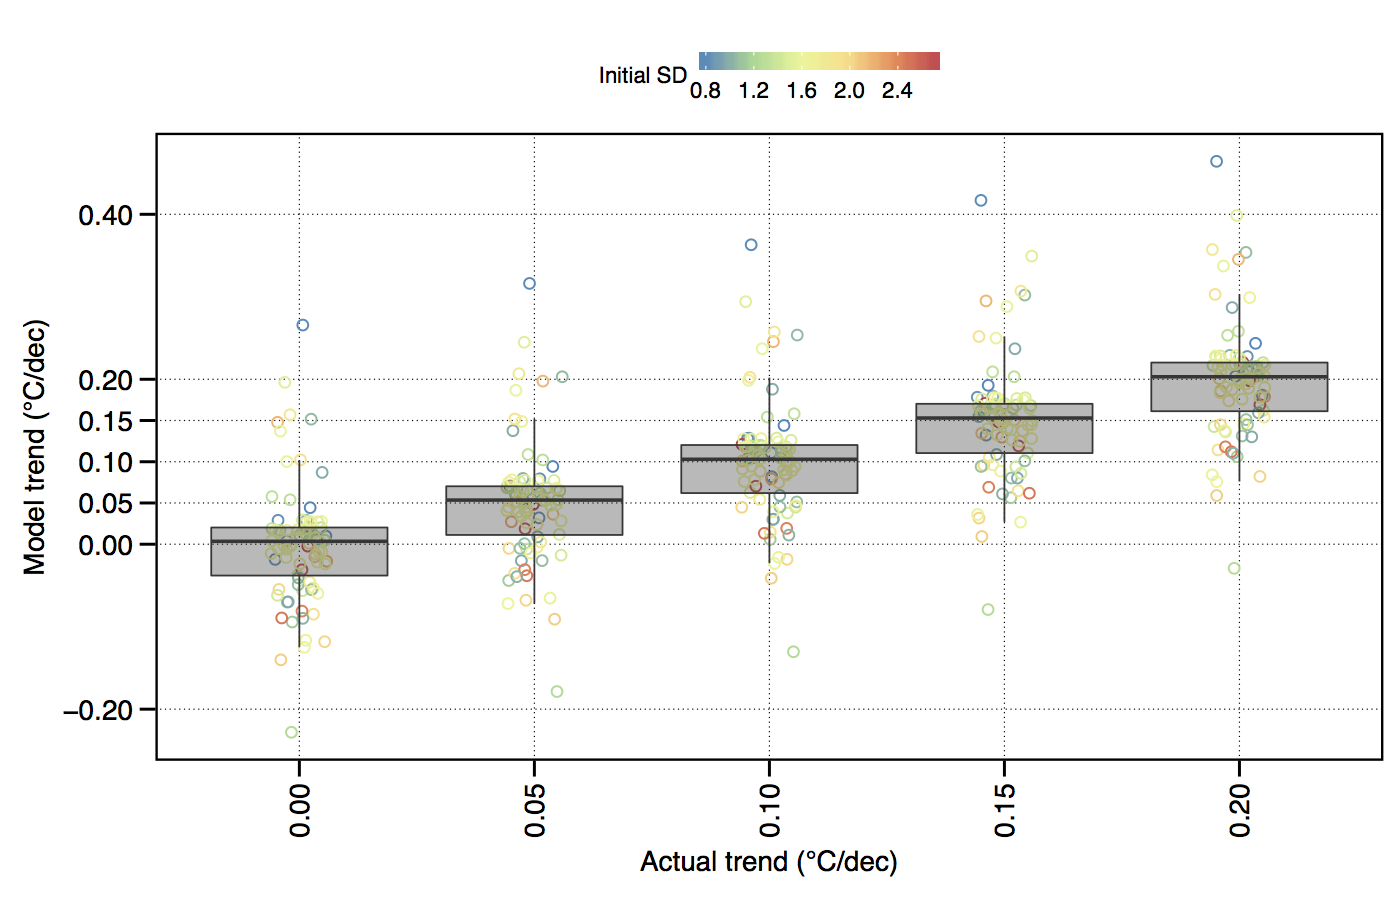
\includegraphics[width=1\linewidth]{figures/all_plt0_no_interp_natural} 

}

\caption{The effect of variance (SD) within a temperature time series on the accurate modelling of decadal trends.}\label{fig:example1}
\end{figure}

\begin{figure}

{\centering 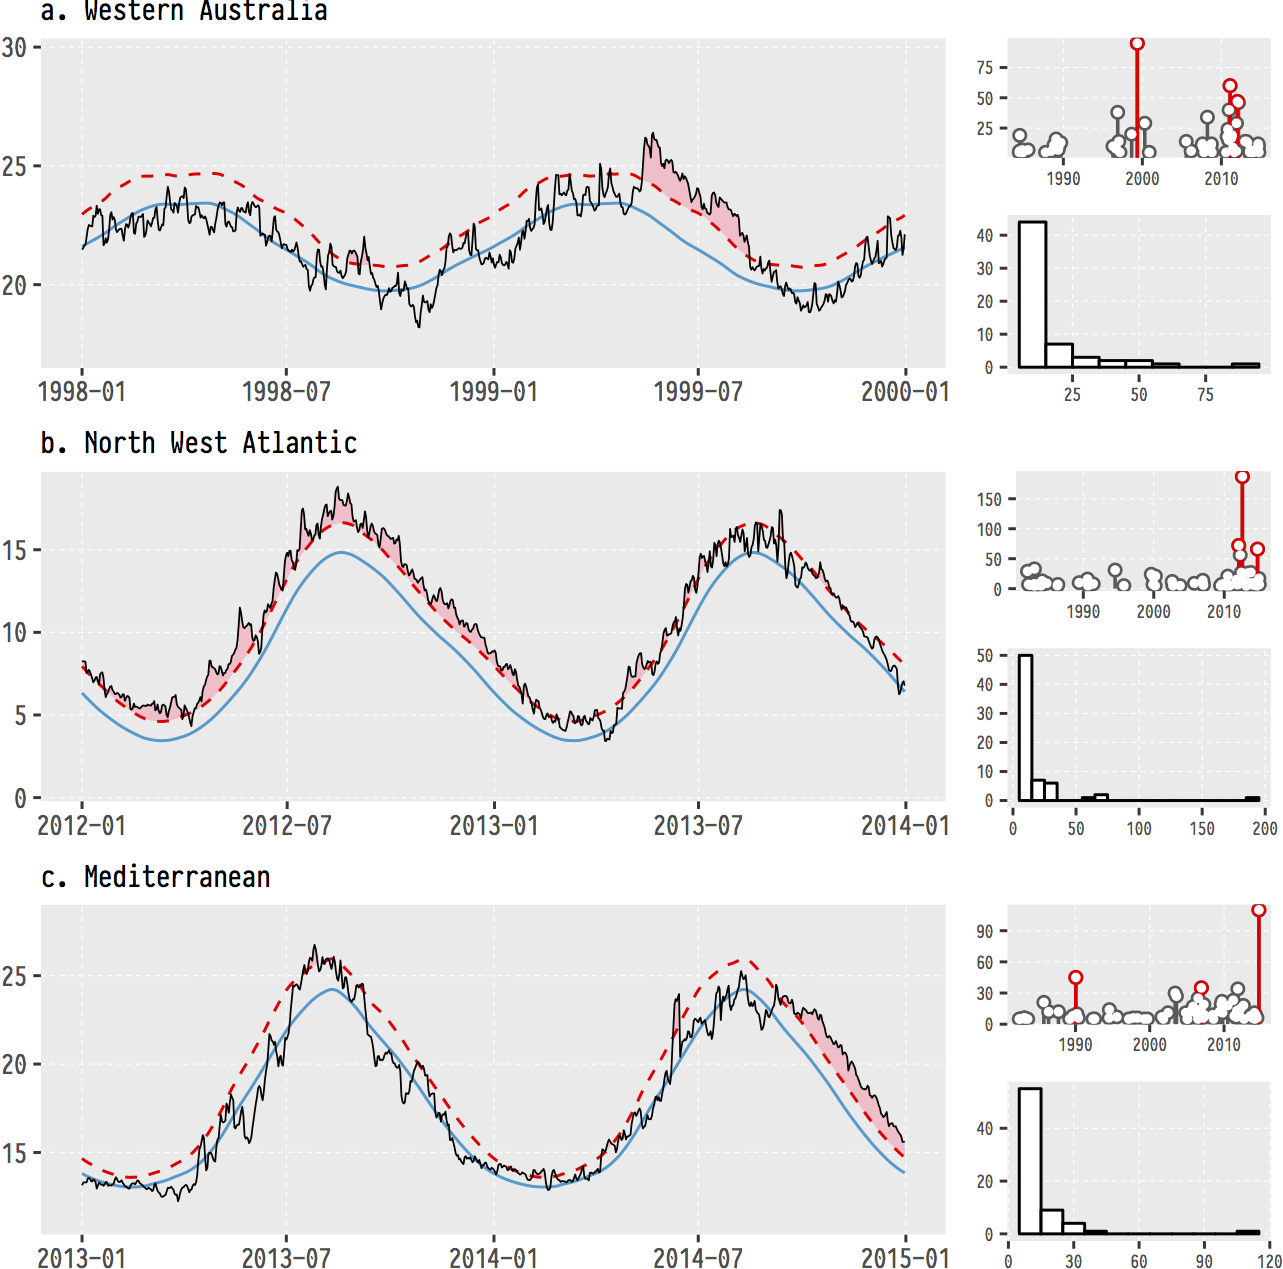
\includegraphics[width=1\linewidth]{figures/deeper-infamous-event-plots-1} 

}

\caption{The (currently) three most infamous marine heatwaves (MHWs) around the world.}\label{fig:example2}
\end{figure}

\begin{figure}

{\centering 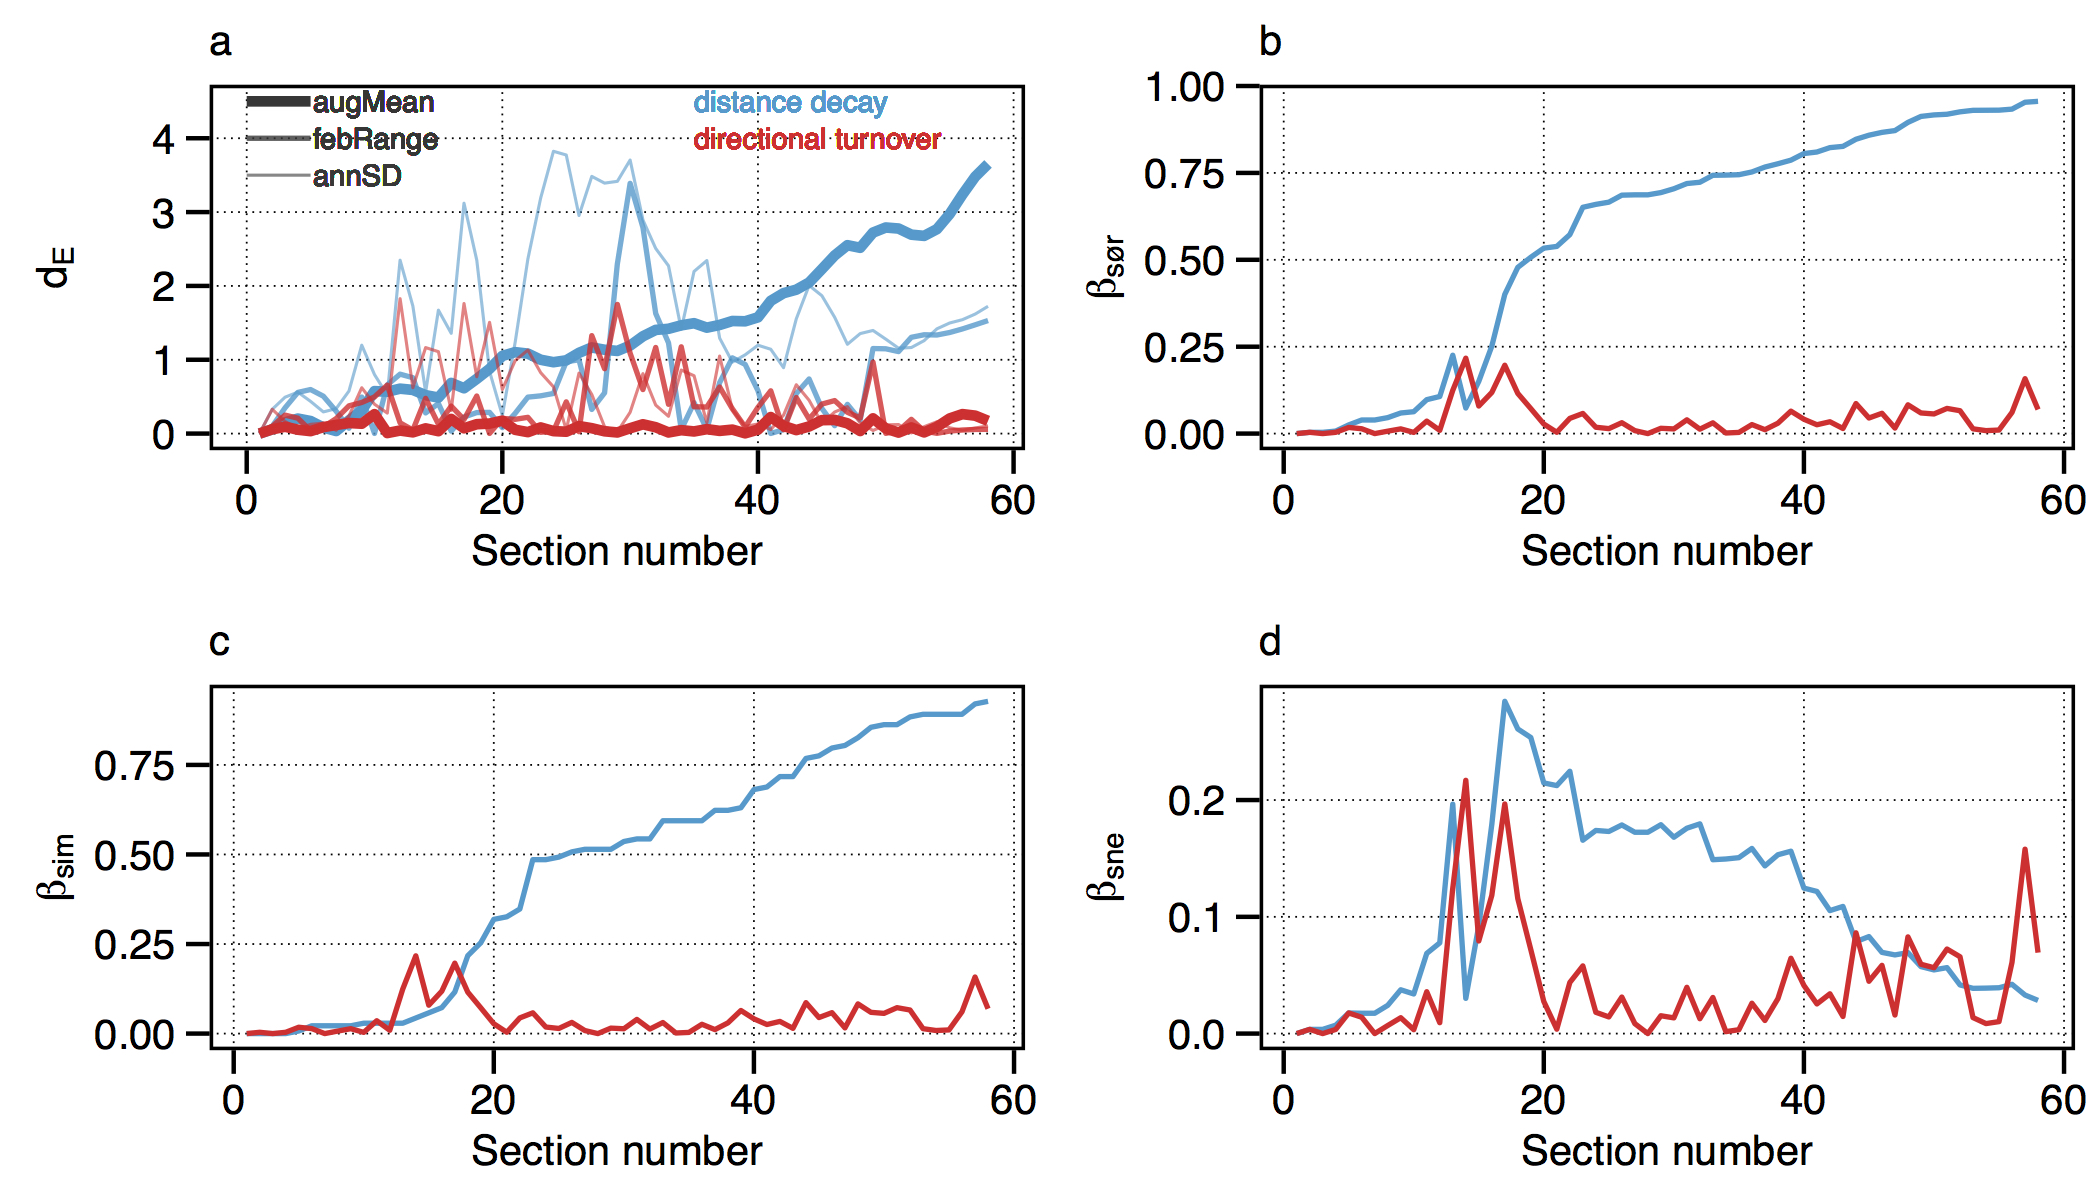
\includegraphics[width=1\linewidth]{figures/Ecography_figure5a-d} 

}

\caption{Changes in seaweed biodiversity along the South African coastline.}\label{fig:example4}
\end{figure}

\begin{figure}

{\centering \includegraphics[width=1\linewidth]{figures/insitu_polarPlots_month_v3.2} 

}

\caption{Polar plots of monthly temperatures.}\label{fig:example16}
\end{figure}

\begin{figure}

{\centering 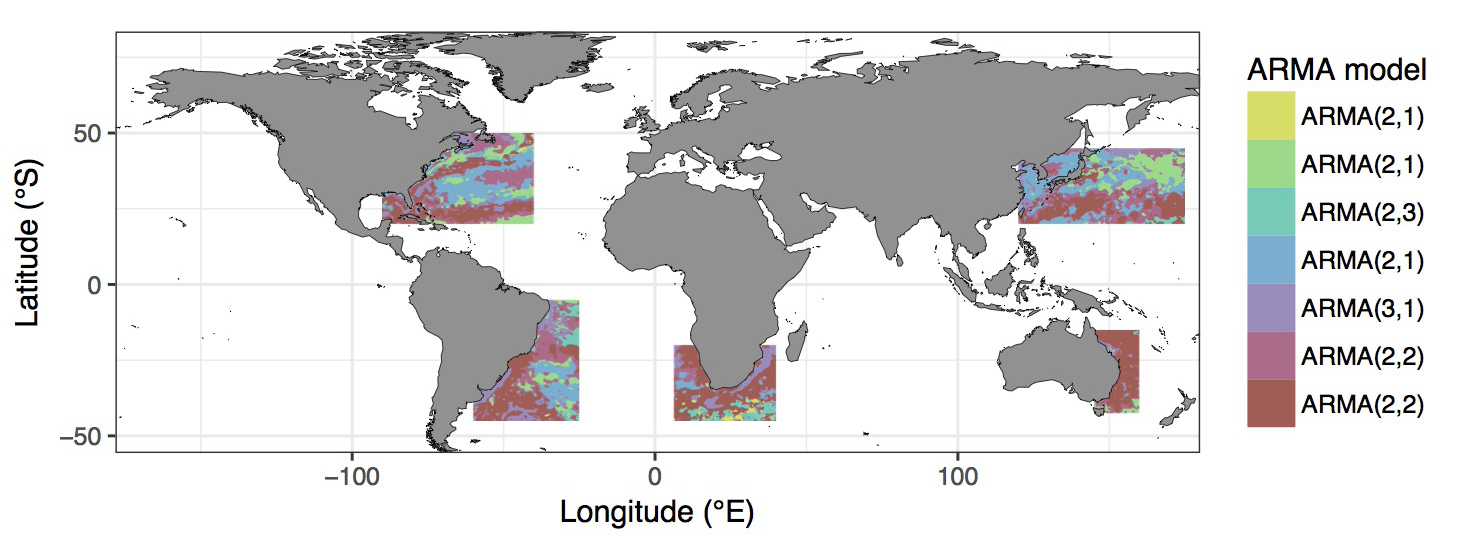
\includegraphics[width=1\linewidth]{figures/mo_coef} 

}

\caption{Most appropriate autoregressive correlation coefficients for areas around western boundary current.}\label{fig:example9}
\end{figure}

\begin{figure}

{\centering 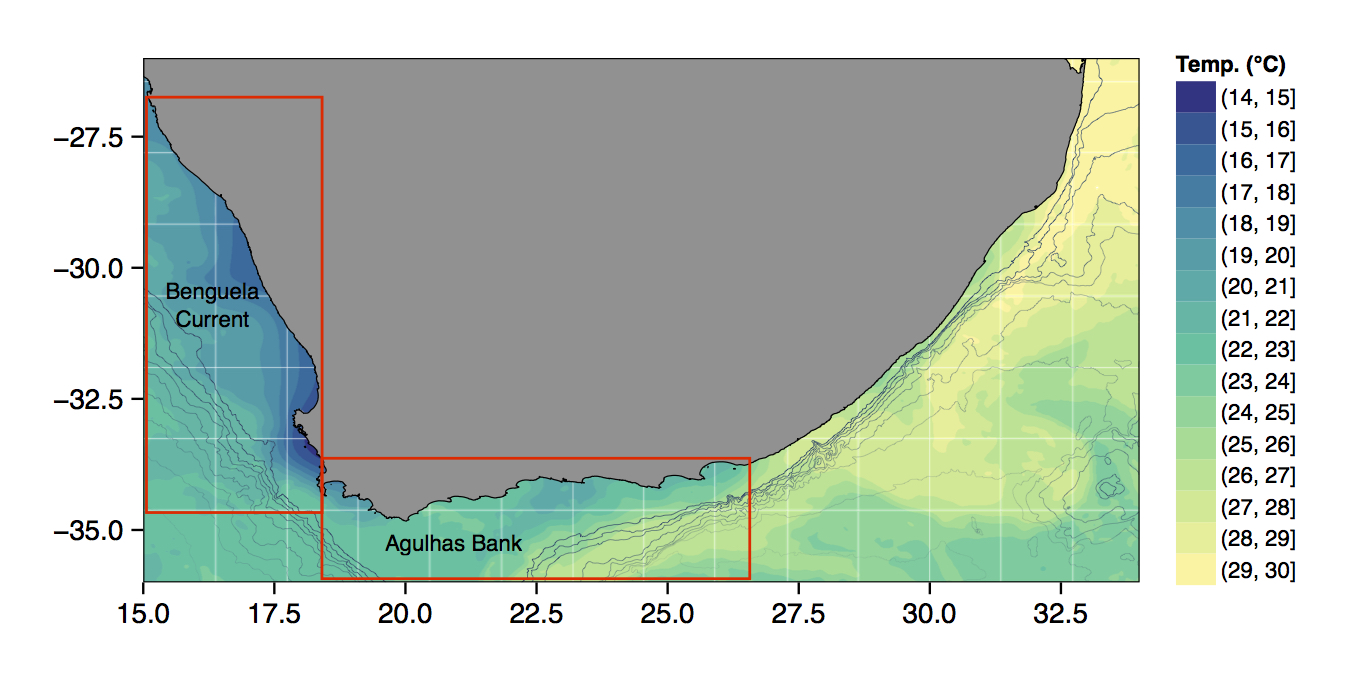
\includegraphics[width=1\linewidth]{figures/MUR_bathy_plot_discrete_20090228} 

}

\caption{The bathymetry of South Africa with SSTs from the MUR product.}\label{fig:example10}
\end{figure}

\begin{figure}

{\centering 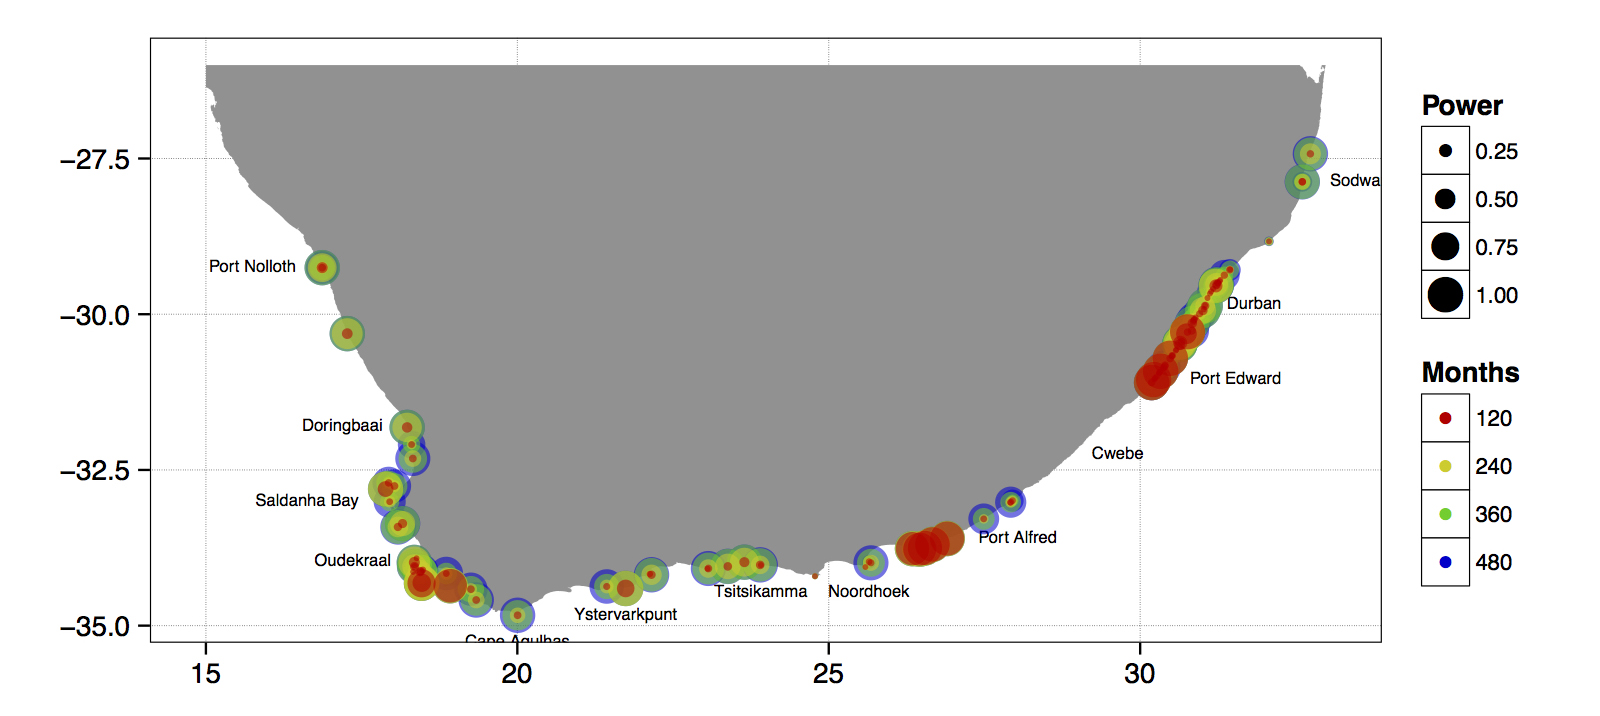
\includegraphics[width=1\linewidth]{figures/sw-fig-7-1} 

}

\caption{The power of the detected decadal trend at each coastal temperature collection site given a hypothetical number of months.}\label{fig:example13}
\end{figure}

\begin{figure}

{\centering 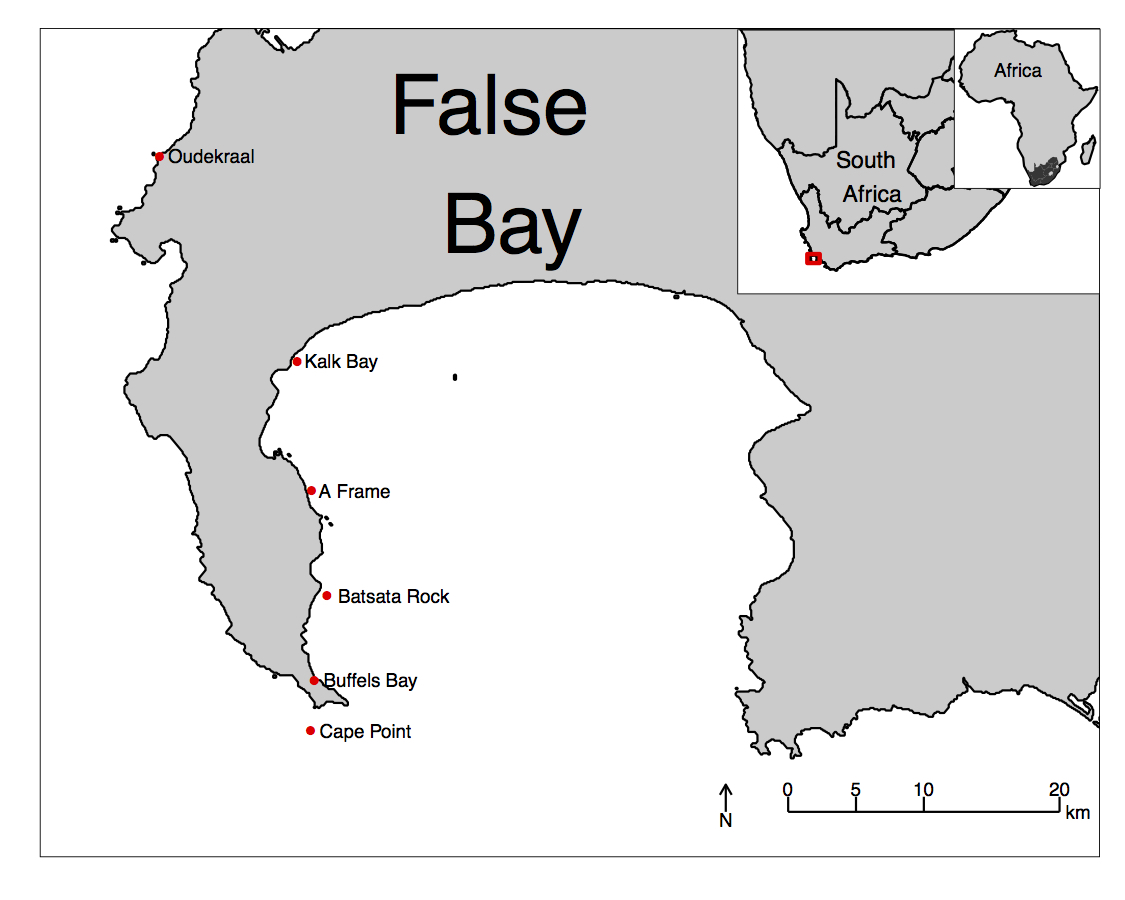
\includegraphics[width=1\linewidth]{figures/false_bay_inset_map_labels2} 

}

\caption{An inset map of False Bay.}\label{fig:example5}
\end{figure}

\begin{figure}

{\centering 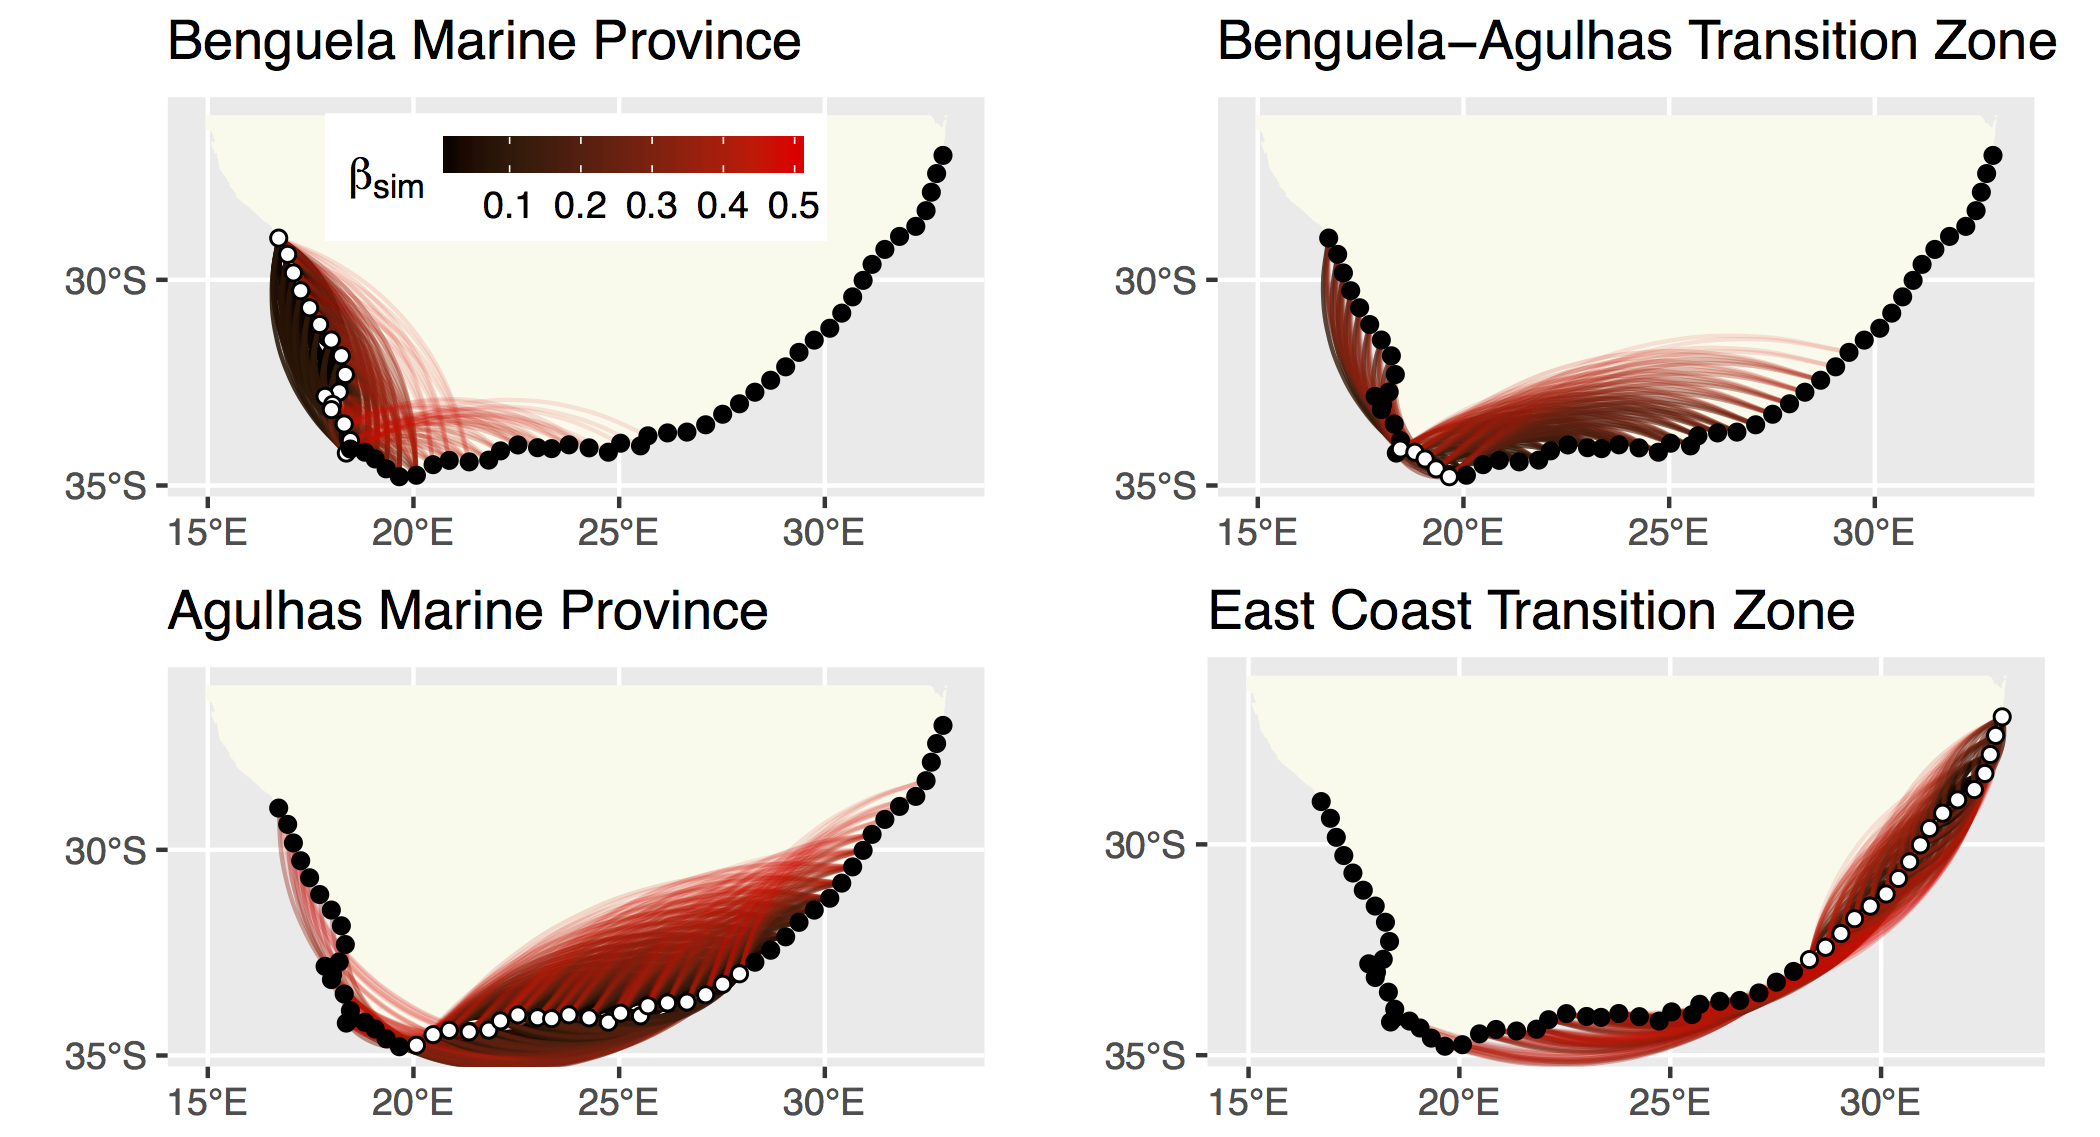
\includegraphics[width=1\linewidth]{figures/PLOS_ONE_Fig4} 

}

\caption{The strength of the relationship between each site based on their biodiversity.}\label{fig:example19}
\end{figure}

\begin{figure}

{\centering 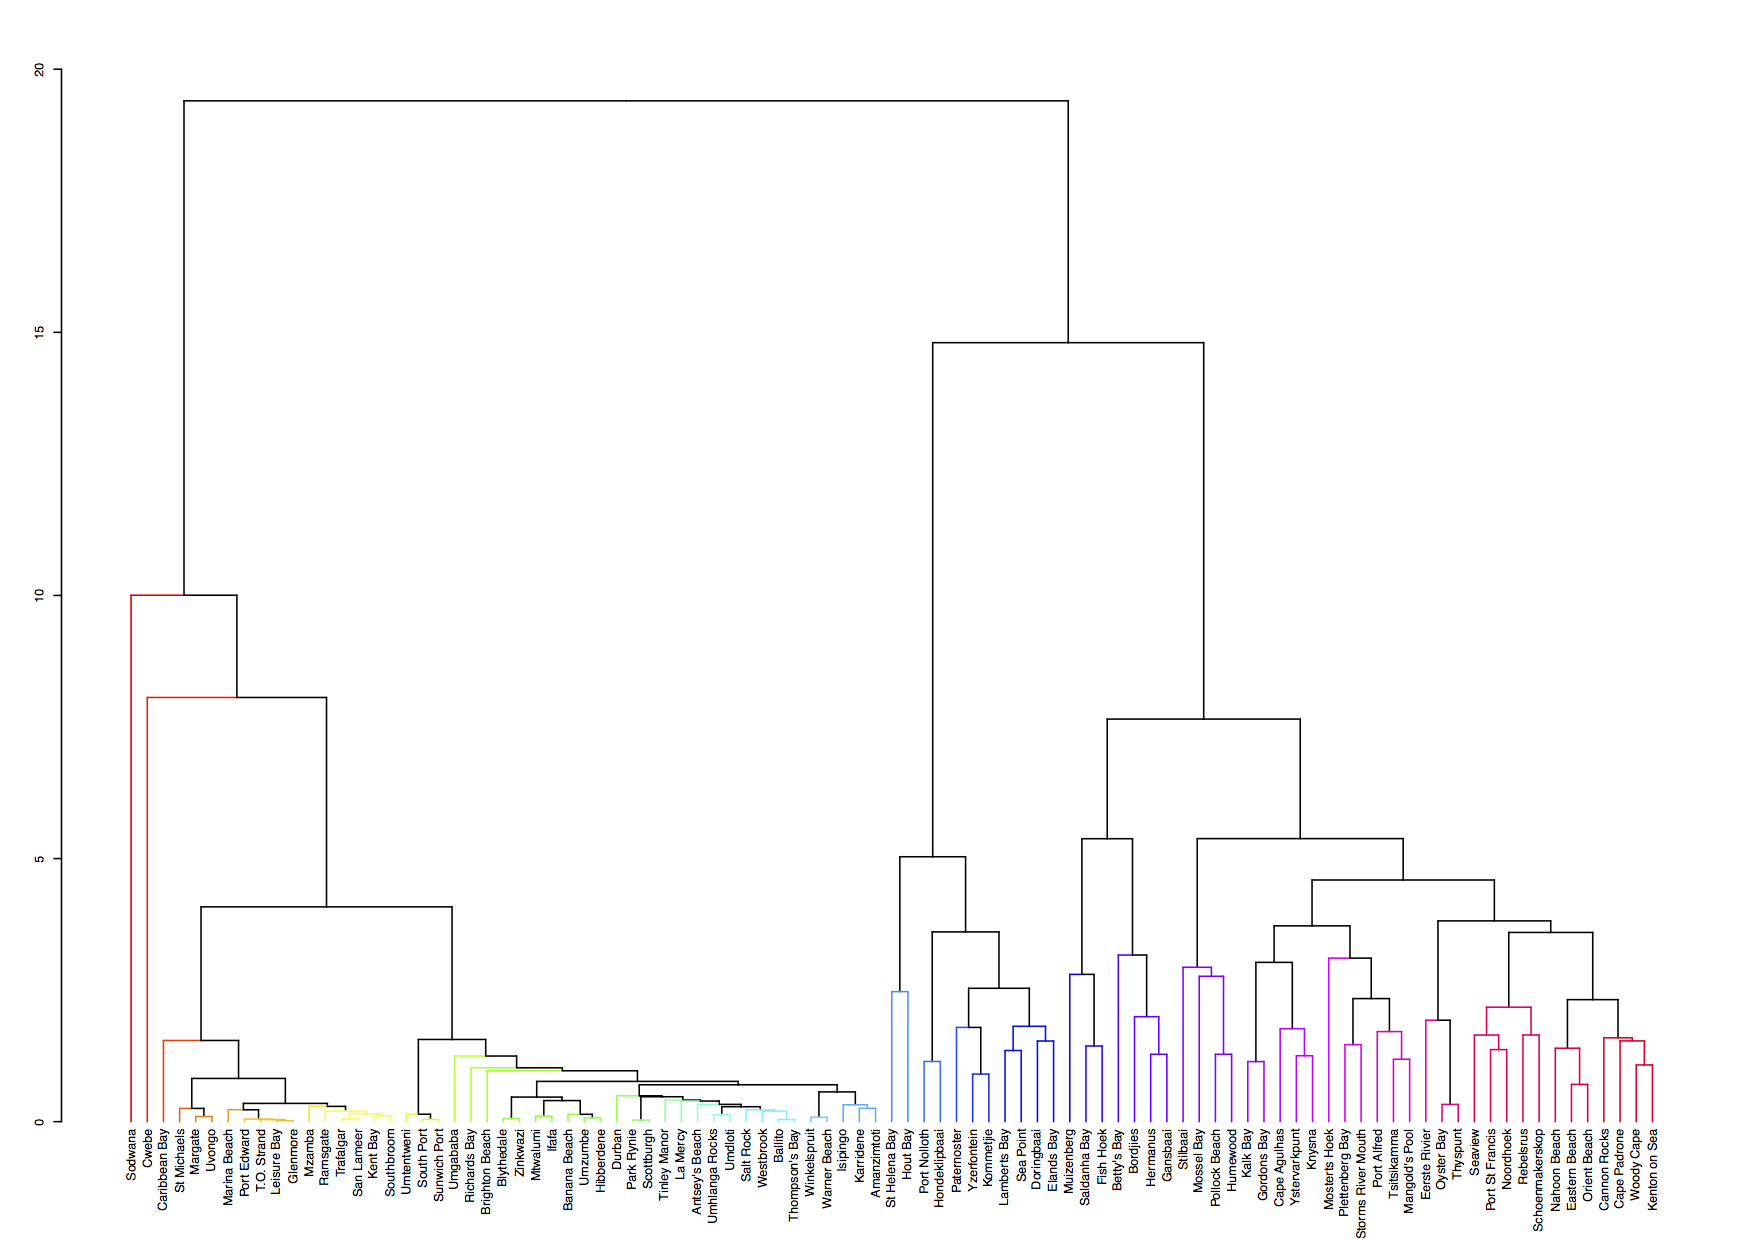
\includegraphics[width=1\linewidth]{figures/hierarchical_clustsig} 

}

\caption{A hierarchical cluster analysis.}\label{fig:example15}
\end{figure}

\begin{figure}

{\centering 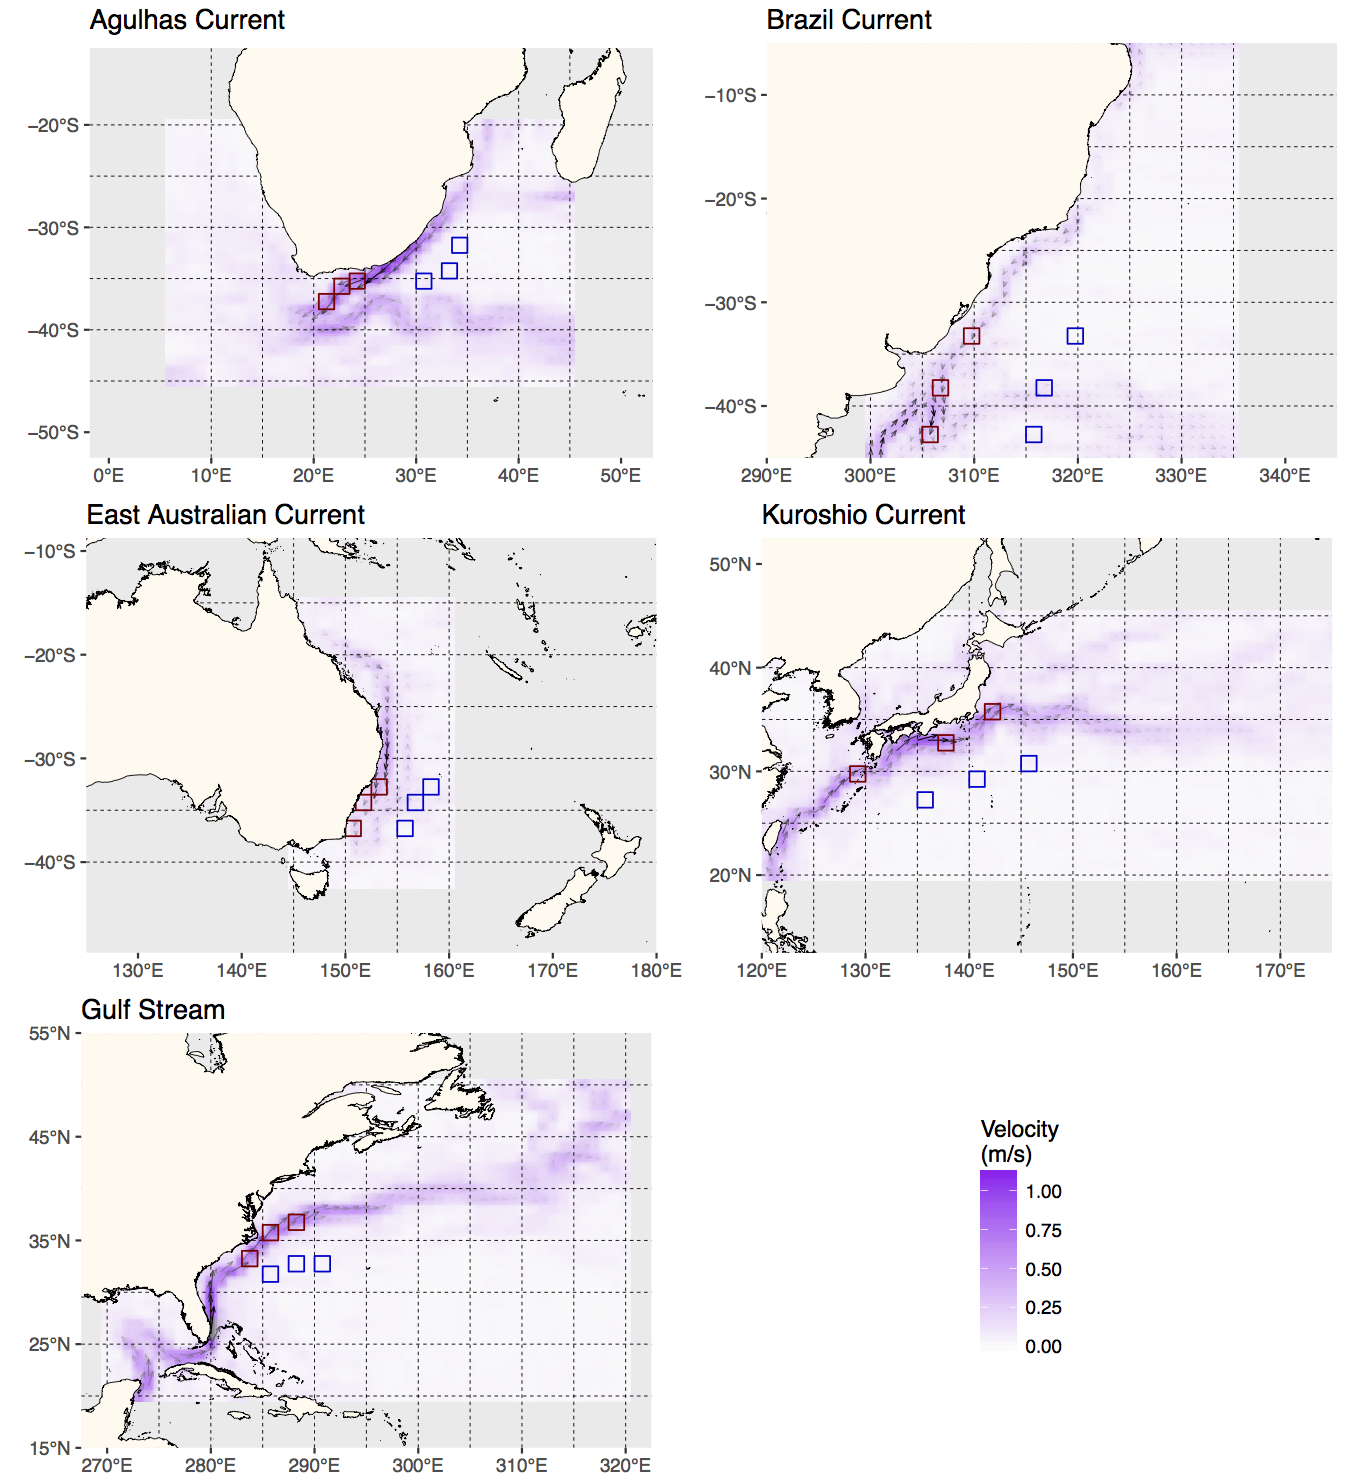
\includegraphics[width=1\linewidth]{figures/Fig01_AvisoMeanVelocityMean} 

}

\caption{Current velcoties of Western Boundary Currents.}\label{fig:example17}
\end{figure}

\hypertarget{basics-of-ggplot2}{%
\section{\texorpdfstring{Basics of \textbf{\texttt{ggplot2}}}{Basics of ggplot2}}\label{basics-of-ggplot2}}

R comes with basic graphing capability, known colloquially (by nerds) as `Base R'. The syntax used for this method of creating graphics is often difficult to interpret as there are few human words in the code. In addition to this issue, Base R also does not allow the user enough control over the look of the final product to satisfy the demands of many publishers. Meaning the figures tend not to look professional enough (but still much better than Excel). To solve both of these problems, and others, the \textbf{\texttt{ggplot2}} package was born.

As part of the \textbf{\texttt{tidyverse}} (as we saw briefly on Day 1, and will go into in depth on Day 4), the \textbf{\texttt{ggplot2}} package endeavours to use a clean, easy for humans to understand syntax that relies heavily on functions that do what they say. For example, the function \texttt{geom\_point()} makes points on a figure. Need a line plot? \texttt{geom\_line()} is the way to go! Need both at the same time? No problem. In \textbf{\texttt{ggplot2}} we may seamlessly merge a nearly limitless number of objects together to create startlingly sophisticated figures. Before we go over the code below, it is very important to note the use of the \texttt{+} signs. When we use \textbf{\texttt{ggplot2}} code we add different lines of code to one another. Each line of code represents one new geometric or aesthetic value of the figure. It is designed this way so as to make it easier for the human eye to read through the code.
One may see below that the code naturally indents itself if the previous line ended with a \texttt{+} sign. This is because R knows that the top line is the parent line and the indented lines are it's children. This is a concept that will come up again when we learn about tidying data. What we need to know now is that a block of code that has \texttt{+} signs, like the one below, must be run together. As long as lines of code end in \texttt{+}, R will assume that you want to keep adding lines of code. If we are not mindful of what we are doing we may tell R to do something it cannot and we will see in the console that R keeps expecting more \texttt{+} signs. If this happens, click inside the console window and push the \texttt{esc} button to cancel the chain of code you are trying to enter.

\begin{Shaded}
\begin{Highlighting}[]
\CommentTok{\# Load libraries}
\KeywordTok{library}\NormalTok{(tidyverse)}

\CommentTok{\# Load data}
\NormalTok{ChickWeight <{-}}\StringTok{ }\NormalTok{datasets}\OperatorTok{::}\NormalTok{ChickWeight}

\CommentTok{\# Create a basic figure}
\KeywordTok{ggplot}\NormalTok{(}\DataTypeTok{data =}\NormalTok{ ChickWeight, }\KeywordTok{aes}\NormalTok{(}\DataTypeTok{x =}\NormalTok{ Time, }\DataTypeTok{y =}\NormalTok{ weight)) }\OperatorTok{+}
\StringTok{  }\KeywordTok{geom\_point}\NormalTok{() }\OperatorTok{+}
\StringTok{  }\KeywordTok{geom\_line}\NormalTok{(}\KeywordTok{aes}\NormalTok{(}\DataTypeTok{group =}\NormalTok{ Chick))}
\end{Highlighting}
\end{Shaded}

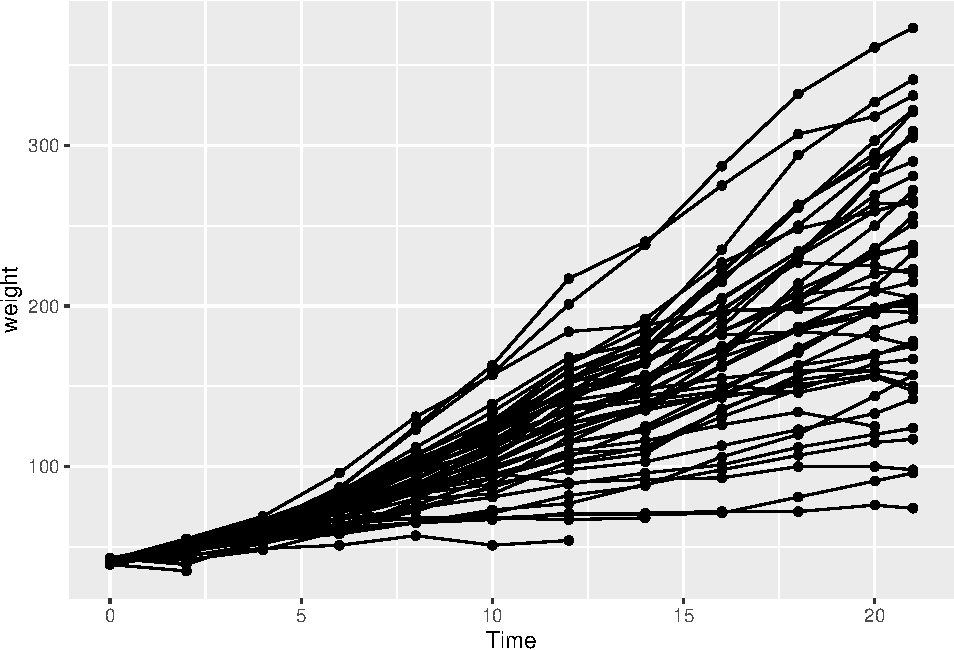
\includegraphics{05-graphics_files/figure-latex/basic-1-1.pdf}

So what is that code doing? We may see from the figure that it is creating a little black dot for every data point, with the \texttt{Time} of sampling on the x axis, and the \texttt{weight} of the chicken during that time on the y axis. It then connects the dots for each chicken in the dataset. Let's break this code down line for line to get a better idea of what it is doing. The first line of code is telling R that we want to create a ggplot figure. We know this because we are using the \texttt{ggplot()} function. Inside of that function we are telling R which dataframe (or tibble) we want to create a figure from. Lastly, with the \texttt{aes()} argument, which is short for `aesthetic', we tell R what the necessary parts of the figure will be. This is also known as `mapping'. The second line of code then takes all of that information and makes points (dots) out of it, added as a layer on the set of axes created by the \texttt{aes()} argument provided within \texttt{ggplot(...)} --- in other words, we add a `geometry' layer, and hence the name of the kind of `shape' we want to plot the data as is prefixed by \texttt{geom\_}. The third line takes the same information and creates lines from it --- it adds yet another layer on top of the pre-existing one. Notice in the third line that we have provided another mapping argument by telling R to group the data by \texttt{Chick}. This is how R knows to draw an individual line for each chicken, and not just one big messy jagged line. Try running this code without the group argument for \texttt{geom\_line()} and see what happens.

This figure doesn't look like much yet. We saw some examples above that show how sophisticated figures may become. This is a remarkably straight forward task. But don't take my word for it, let's see for ourselves. By adding one more aesthetic to the code above we will now show each \texttt{Diet} as a different colour.

\begin{Shaded}
\begin{Highlighting}[]
\KeywordTok{ggplot}\NormalTok{(}\DataTypeTok{data =}\NormalTok{ ChickWeight, }\KeywordTok{aes}\NormalTok{(}\DataTypeTok{x =}\NormalTok{ Time, }\DataTypeTok{y =}\NormalTok{ weight, }\DataTypeTok{colour =}\NormalTok{ Diet)) }\OperatorTok{+}
\StringTok{  }\KeywordTok{geom\_point}\NormalTok{() }\OperatorTok{+}
\StringTok{  }\KeywordTok{geom\_line}\NormalTok{(}\KeywordTok{aes}\NormalTok{(}\DataTypeTok{group =}\NormalTok{ Chick))}
\end{Highlighting}
\end{Shaded}

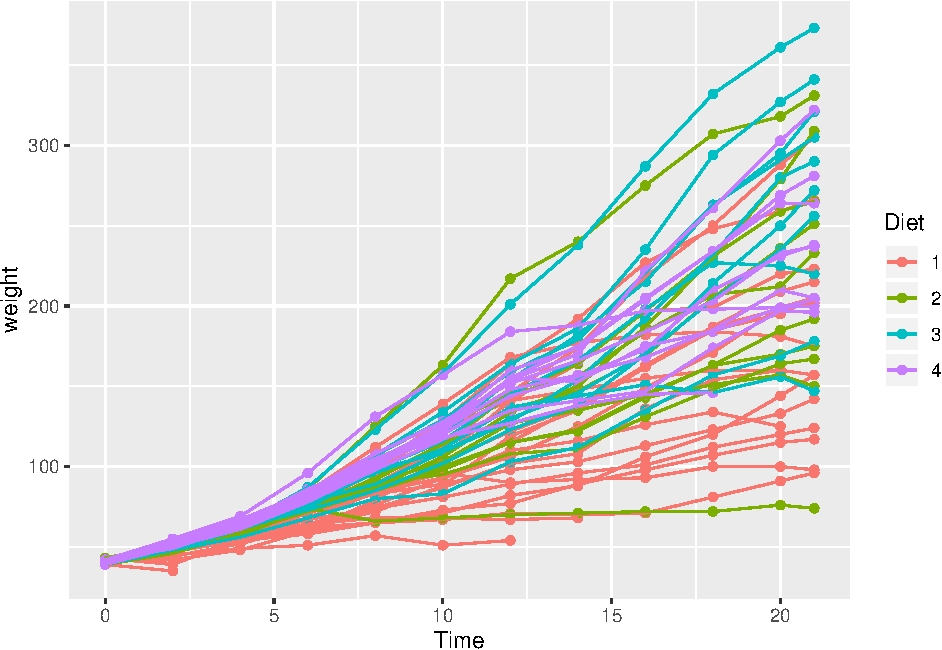
\includegraphics{05-graphics_files/figure-latex/basic-3-1.pdf}

Do any patterns appear to emerge from the data? Perhaps there is a better way to visualise them? With linear models for example.

\begin{Shaded}
\begin{Highlighting}[]
\KeywordTok{ggplot}\NormalTok{(}\DataTypeTok{data =}\NormalTok{ ChickWeight, }\KeywordTok{aes}\NormalTok{(}\DataTypeTok{x =}\NormalTok{ Time, }\DataTypeTok{y =}\NormalTok{ weight, }\DataTypeTok{colour =}\NormalTok{ Diet)) }\OperatorTok{+}
\StringTok{  }\KeywordTok{geom\_point}\NormalTok{() }\OperatorTok{+}
\StringTok{  }\KeywordTok{geom\_smooth}\NormalTok{(}\DataTypeTok{method =} \StringTok{"lm"}\NormalTok{)}
\end{Highlighting}
\end{Shaded}

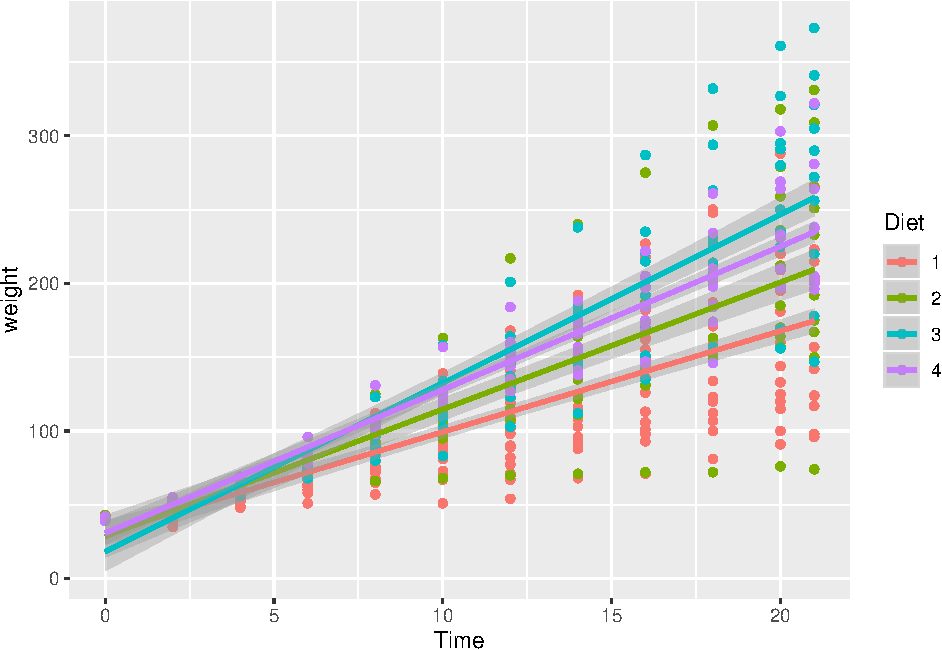
\includegraphics{05-graphics_files/figure-latex/first-lm-1.pdf}

How is a linear model calculated? What patterns do we see in the data now? If you were a chicken, which feed would you want?

\hypertarget{to-aes-or-not-to-aes-that-is-the-question}{%
\section{\texorpdfstring{To \texttt{aes()} or not to \texttt{aes()}, that is the question}{To aes() or not to aes(), that is the question}}\label{to-aes-or-not-to-aes-that-is-the-question}}

The astute eye will have noticed by now that most arguments we have added to the code have been inside of the \texttt{aes()} function. So what exactly is that \texttt{aes()} function doing sitting inside of the other functions? The reason for the \texttt{aes()} function is that it controls the look of the other functions dynamically based on the variables you provide it. If we want to change the look of the plot by some static value we would do this by passing the argument for that variable to the geom of our choosing \emph{outside} of the \texttt{aes()} function. Let's see what this looks like by changing the colour of the dots.

\begin{Shaded}
\begin{Highlighting}[]
\KeywordTok{ggplot}\NormalTok{(}\DataTypeTok{data =}\NormalTok{ ChickWeight, }\KeywordTok{aes}\NormalTok{(}\DataTypeTok{x =}\NormalTok{ Time, }\DataTypeTok{y =}\NormalTok{ weight)) }\OperatorTok{+}
\StringTok{  }\KeywordTok{geom\_point}\NormalTok{(}\DataTypeTok{colour =} \StringTok{"blue"}\NormalTok{) }\OperatorTok{+}
\StringTok{  }\KeywordTok{geom\_line}\NormalTok{(}\KeywordTok{aes}\NormalTok{(}\DataTypeTok{group =}\NormalTok{ Chick, }\DataTypeTok{colour =} \StringTok{"blue"}\NormalTok{))}
\end{Highlighting}
\end{Shaded}

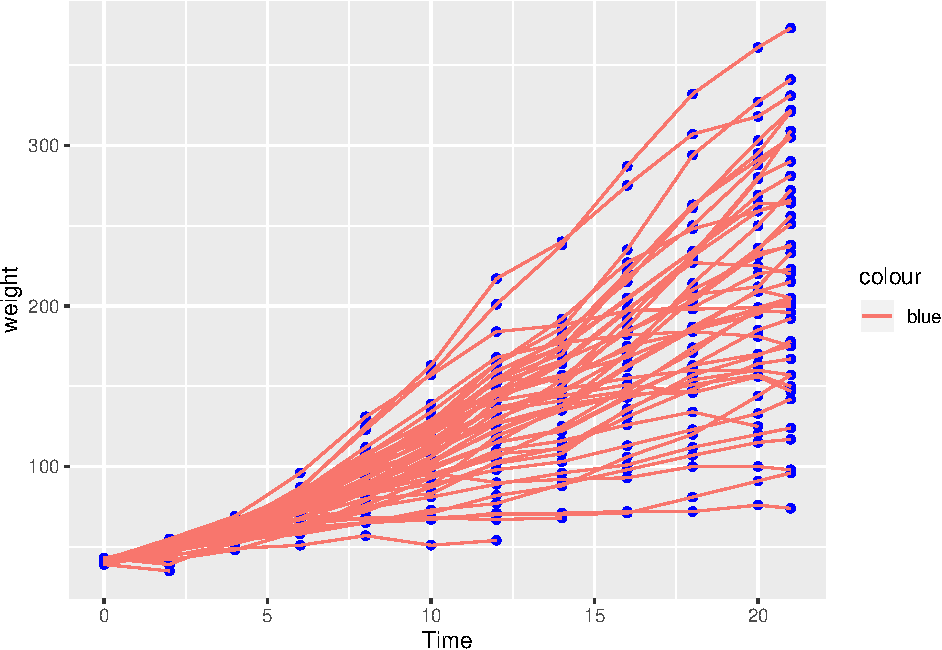
\includegraphics{05-graphics_files/figure-latex/basic-6-1.pdf}

Why are the points blue, but the lines are salmon with a legend that says they are `blue'? We may see that in the line responsible for the points (\texttt{geom\_point()}) we did not put the colour argument inside of the \texttt{aes()} function, but for the lines (\texttt{geom\_line()}) we did. If we know that we want some aspect of our figure to be a static value we set this value outside of the \texttt{aes()} function. If we want some aspect of our figure to reflect some part of the data in our dataframe, we must set that inside of \texttt{aes()}. Let's see an example where we set the size of the dots to equal the weight of the chicken and the thickness of the linear model lines to one static value.

\begin{Shaded}
\begin{Highlighting}[]
\KeywordTok{ggplot}\NormalTok{(}\DataTypeTok{data =}\NormalTok{ ChickWeight, }\KeywordTok{aes}\NormalTok{(}\DataTypeTok{x =}\NormalTok{ Time, }\DataTypeTok{y =}\NormalTok{ weight, }\DataTypeTok{colour =}\NormalTok{ Diet)) }\OperatorTok{+}
\StringTok{  }\KeywordTok{geom\_point}\NormalTok{(}\KeywordTok{aes}\NormalTok{(}\DataTypeTok{size =}\NormalTok{ weight)) }\OperatorTok{+}
\StringTok{  }\KeywordTok{geom\_smooth}\NormalTok{(}\DataTypeTok{method =} \StringTok{"lm"}\NormalTok{, }\DataTypeTok{size =} \FloatTok{1.2}\NormalTok{)}
\end{Highlighting}
\end{Shaded}

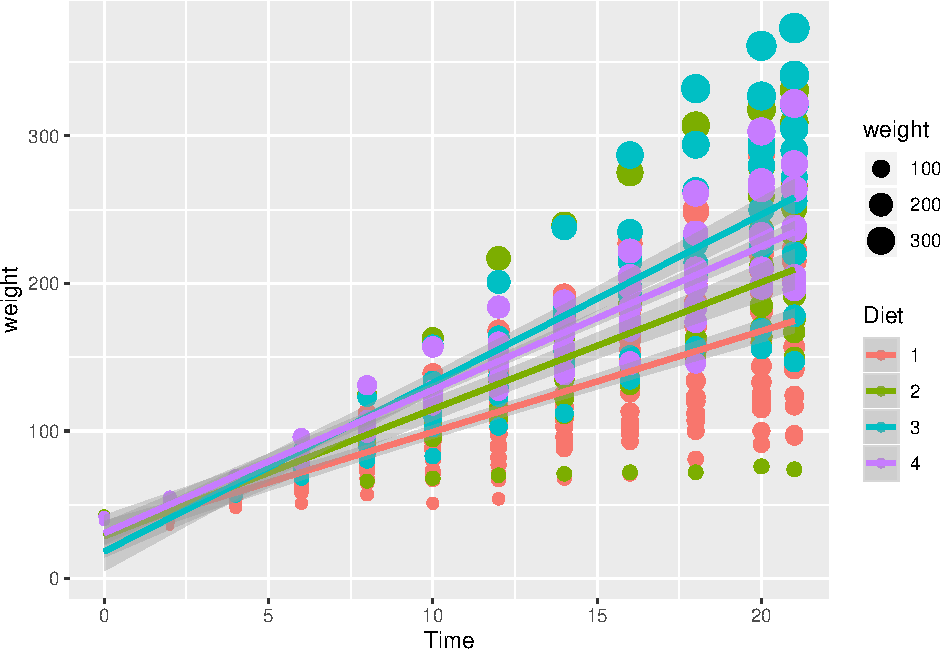
\includegraphics{05-graphics_files/figure-latex/basic-8-1.pdf}

Notice that we have set the size of the points and the lines, but one is within \texttt{aes()} and the other not. Because the size of our points equals the weight of the chickens, the points become larger the heavier (juicier) the chickens become. But because we set the size of the lines to one static value, all of the lines are the same size and don't change because of any other variables.

\hypertarget{changing-labels}{%
\section{Changing labels}\label{changing-labels}}

When we use \textbf{\texttt{ggplot2}} we have control over every minute aspect of our figures if we so wish. What we want to do next is put the legend on the bottom of our figure with a horizontal orientation and change the axis labels so that they show the units of measurement. To change the labels we will need the \texttt{labs()} function. To change the position of the legend we need the \texttt{theme()} function as it is within this function that all of the little tweaks are performed. This is best placed at the end of your block of \textbf{\texttt{ggplot2}} code.

\begin{Shaded}
\begin{Highlighting}[]
\KeywordTok{ggplot}\NormalTok{(}\DataTypeTok{data =}\NormalTok{ ChickWeight, }\KeywordTok{aes}\NormalTok{(}\DataTypeTok{x =}\NormalTok{ Time, }\DataTypeTok{y =}\NormalTok{ weight, }\DataTypeTok{colour =}\NormalTok{ Diet)) }\OperatorTok{+}
\StringTok{  }\KeywordTok{geom\_point}\NormalTok{() }\OperatorTok{+}
\StringTok{  }\KeywordTok{geom\_smooth}\NormalTok{(}\DataTypeTok{method =} \StringTok{"lm"}\NormalTok{) }\OperatorTok{+}
\StringTok{  }\KeywordTok{labs}\NormalTok{(}\DataTypeTok{x =} \StringTok{"Days"}\NormalTok{, }\DataTypeTok{y =} \StringTok{"Mass (g)"}\NormalTok{, }\DataTypeTok{colour =} \StringTok{"diet type"}\NormalTok{) }\OperatorTok{+}\StringTok{ }\CommentTok{\# Change the labels}
\StringTok{  }\KeywordTok{theme}\NormalTok{(}\DataTypeTok{legend.position =} \StringTok{"bottom"}\NormalTok{) }\CommentTok{\# Change the legend position}
\end{Highlighting}
\end{Shaded}

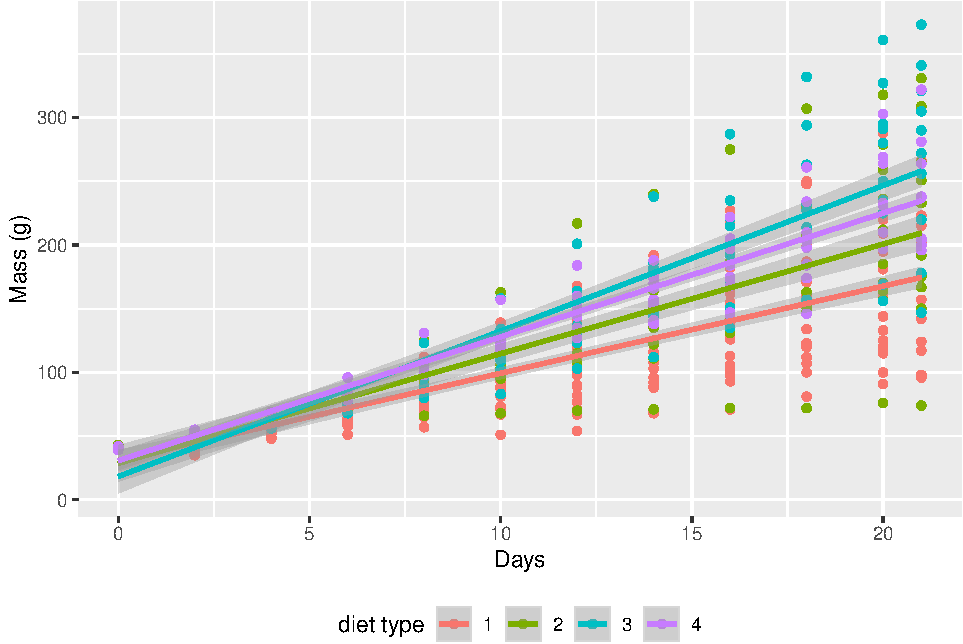
\includegraphics{05-graphics_files/figure-latex/basic-4-1.pdf}

Notice that when we place the legend at the bottom of the figure ggplot automatically makes it horizontal for us. Why do we use `colour' inside of \texttt{labs()} to change the legend title?

\hypertarget{exercise-3}{%
\chapter{Exercise:}\label{exercise-3}}

With all of this information in hand, please take another five minutes to either improve one of the plots generated or create a beautiful graph of your own. Here are some ideas:

\begin{itemize}
\tightlist
\item
  See if you can change the thickness of the points/lines.
\item
  Change the shape, colour, fill and size of each of the points.
\item
  Can you find a way to change the name of the legend? What about its labels?
\item
  Explore the different geom functions available. These include geom\_boxplot, geom\_density, etc.
\item
  Try using a different color palette
\item
  Use different themes
\end{itemize}

\hypertarget{session-info-3}{%
\section{Session info}\label{session-info-3}}

\begin{Shaded}
\begin{Highlighting}[]
\KeywordTok{installed.packages}\NormalTok{()[}\KeywordTok{names}\NormalTok{(}\KeywordTok{sessionInfo}\NormalTok{()}\OperatorTok{$}\NormalTok{otherPkgs), }\StringTok{"Version"}\NormalTok{]}
\end{Highlighting}
\end{Shaded}

\begin{verbatim}
R>   forcats   stringr     dplyr     purrr     readr     tidyr    tibble   ggplot2 
R>   "0.4.0"   "1.4.0"   "0.8.3"   "0.3.3"   "1.3.1"   "1.0.0"   "2.1.3"   "3.2.1" 
R> tidyverse 
R>   "1.3.0"
\end{verbatim}

\hypertarget{faceting}{%
\chapter{Faceting Figures}\label{faceting}}

\begin{quote}
``But let the mind beware, that though the flesh be bugged, the circumstances of existence are pretty glorious.''

--- Kurt Vonnegut, Player Piano
\end{quote}

\begin{quote}
``You miss 100\% of the shots you don't take.''

--- Wayne Gretzky
\end{quote}

So far we have only looked at single panel figures. But as you may have guessed by now, \textbf{\texttt{ggplot2}} is capable of creating any sort of data visualisation that a human mind could conceive. This may seem like a grandiose assertion, but we'll see if we can't convince you of it by the end of this course. For now however, let's just take our understanding of the usability of \textbf{\texttt{ggplot2}} two steps further by first learning how to facet a single figure, and then stitch different types of figures together into a grid. In order to aid us in this process we will make use of an additional package, \textbf{\texttt{ggpubr}}. The purpose of this package is to provide a bevy of additional tools that researchers commonly make use of in order to produce publication quality figures. Note that \texttt{library(ggpubr)} will not work on your computer if you have not yet installed the package.

\begin{Shaded}
\begin{Highlighting}[]
\CommentTok{\# Load libraries}
\KeywordTok{library}\NormalTok{(tidyverse)}
\KeywordTok{library}\NormalTok{(ggpubr)}
\end{Highlighting}
\end{Shaded}

\hypertarget{faceting-one-figure}{%
\section{Faceting one figure}\label{faceting-one-figure}}

Faceting a single figure is built into \textbf{\texttt{ggplot2}} from the ground up and will work with virtually anything that could be passed to the \texttt{aes()} function. Here we see how to create an individual facet for each \texttt{Diet} within the \texttt{ChickWeight} dataset.

\begin{Shaded}
\begin{Highlighting}[]
\CommentTok{\# Load data}
\NormalTok{ChickWeight <{-}}\StringTok{ }\NormalTok{datasets}\OperatorTok{::}\NormalTok{ChickWeight}

\CommentTok{\# Create faceted figure}
\KeywordTok{ggplot}\NormalTok{(}\DataTypeTok{data =}\NormalTok{ ChickWeight, }\KeywordTok{aes}\NormalTok{(}\DataTypeTok{x =}\NormalTok{ Time, }\DataTypeTok{y =}\NormalTok{ weight, }\DataTypeTok{colour =}\NormalTok{ Diet)) }\OperatorTok{+}
\StringTok{  }\KeywordTok{geom\_point}\NormalTok{() }\OperatorTok{+}
\StringTok{  }\KeywordTok{geom\_smooth}\NormalTok{(}\DataTypeTok{method =} \StringTok{"lm"}\NormalTok{) }\OperatorTok{+}\StringTok{ }\CommentTok{\# Note the \textasciigrave{}+\textasciigrave{} sign here}
\StringTok{  }\KeywordTok{facet\_wrap}\NormalTok{(}\OperatorTok{\textasciitilde{}}\NormalTok{Diet, }\DataTypeTok{ncol =} \DecValTok{2}\NormalTok{) }\OperatorTok{+}\StringTok{ }\CommentTok{\# This is the line that creates the facets}
\StringTok{  }\KeywordTok{labs}\NormalTok{(}\DataTypeTok{x =} \StringTok{"Days"}\NormalTok{, }\DataTypeTok{y =} \StringTok{"Mass (g)"}\NormalTok{)}
\end{Highlighting}
\end{Shaded}

\begin{figure}
\centering
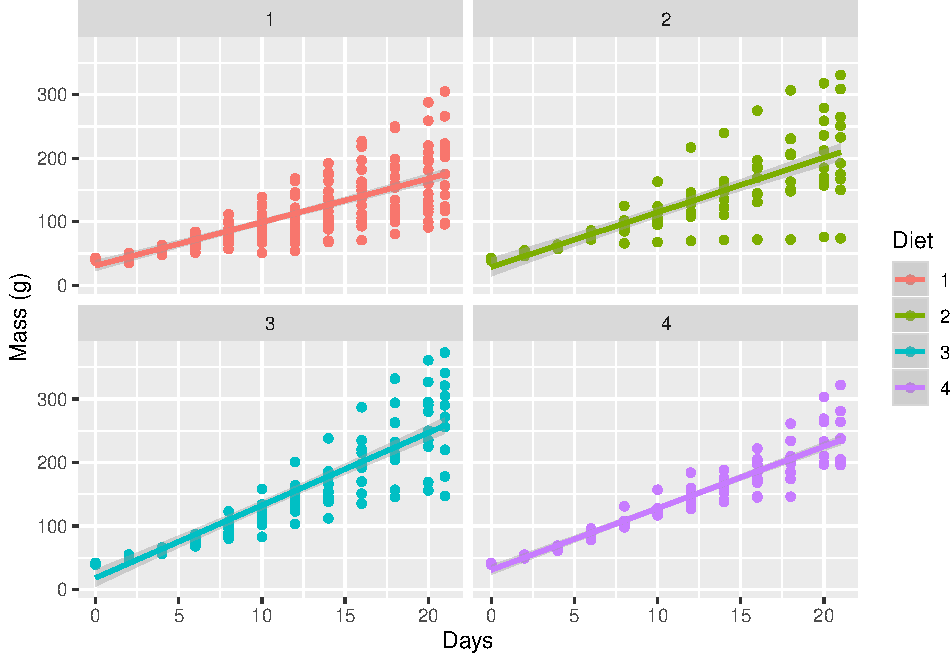
\includegraphics{06-faceting_files/figure-latex/facet-1-1.pdf}
\caption{\label{fig:facet-1}Simple faceted figure showing a linear model applied to each diet.}
\end{figure}

\hypertarget{new-figure-types}{%
\section{New figure types}\label{new-figure-types}}

Before we can create a gridded figure of several smaller figures, we need to learn how to create a few new types of figures first. The code for these different types is shown below. Some of the figure types we will learn how to use now do not work well with the full \texttt{ChickWeight} dataset. Rather we will want only the weights from the final day of collection. To filter only these data we will need to use a bit of the `tidy' code we saw on Day 1.

\begin{Shaded}
\begin{Highlighting}[]
\NormalTok{ChickLast <{-}}\StringTok{ }\NormalTok{ChickWeight }\OperatorTok{\%>\%}\StringTok{ }
\StringTok{  }\KeywordTok{filter}\NormalTok{(Time }\OperatorTok{==}\StringTok{ }\DecValTok{21}\NormalTok{)}
\end{Highlighting}
\end{Shaded}

\hypertarget{line-graph}{%
\subsection{Line graph}\label{line-graph}}

\begin{Shaded}
\begin{Highlighting}[]
\NormalTok{line\_}\DecValTok{1}\NormalTok{ <{-}}\StringTok{ }\KeywordTok{ggplot}\NormalTok{(}\DataTypeTok{data =}\NormalTok{ ChickWeight, }\KeywordTok{aes}\NormalTok{(}\DataTypeTok{x =}\NormalTok{ Time, }\DataTypeTok{y =}\NormalTok{ weight, }\DataTypeTok{colour =}\NormalTok{ Diet)) }\OperatorTok{+}
\StringTok{  }\KeywordTok{geom\_point}\NormalTok{() }\OperatorTok{+}
\StringTok{  }\KeywordTok{geom\_line}\NormalTok{(}\KeywordTok{aes}\NormalTok{(}\DataTypeTok{group =}\NormalTok{ Chick)) }\OperatorTok{+}
\StringTok{  }\KeywordTok{labs}\NormalTok{(}\DataTypeTok{x =} \StringTok{"Days"}\NormalTok{, }\DataTypeTok{y =} \StringTok{"Mass (g)"}\NormalTok{)}
\NormalTok{line\_}\DecValTok{1}
\end{Highlighting}
\end{Shaded}

\begin{figure}
\centering
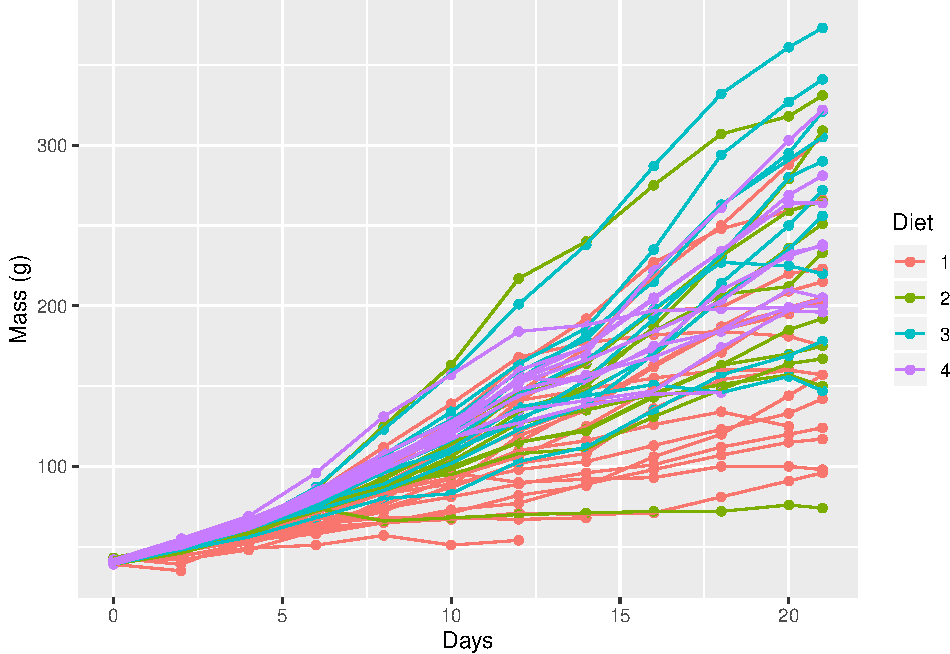
\includegraphics{06-faceting_files/figure-latex/facet-line-1.pdf}
\caption{\label{fig:facet-line}Line graph for the progression of chicken weights (g) over time (days) based on four different diets.}
\end{figure}

\hypertarget{linear-model}{%
\subsection{Linear model}\label{linear-model}}

\begin{Shaded}
\begin{Highlighting}[]
\NormalTok{lm\_}\DecValTok{1}\NormalTok{ <{-}}\StringTok{ }\KeywordTok{ggplot}\NormalTok{(}\DataTypeTok{data =}\NormalTok{ ChickWeight, }\KeywordTok{aes}\NormalTok{(}\DataTypeTok{x =}\NormalTok{ Time, }\DataTypeTok{y =}\NormalTok{ weight, }\DataTypeTok{colour =}\NormalTok{ Diet)) }\OperatorTok{+}
\StringTok{  }\KeywordTok{geom\_point}\NormalTok{() }\OperatorTok{+}
\StringTok{  }\KeywordTok{geom\_smooth}\NormalTok{(}\DataTypeTok{method =} \StringTok{"gam"}\NormalTok{) }\OperatorTok{+}
\StringTok{  }\KeywordTok{labs}\NormalTok{(}\DataTypeTok{x =} \StringTok{"Days"}\NormalTok{, }\DataTypeTok{y =} \StringTok{"Mass (g)"}\NormalTok{)}
\NormalTok{lm\_}\DecValTok{1}
\end{Highlighting}
\end{Shaded}

\begin{figure}
\centering
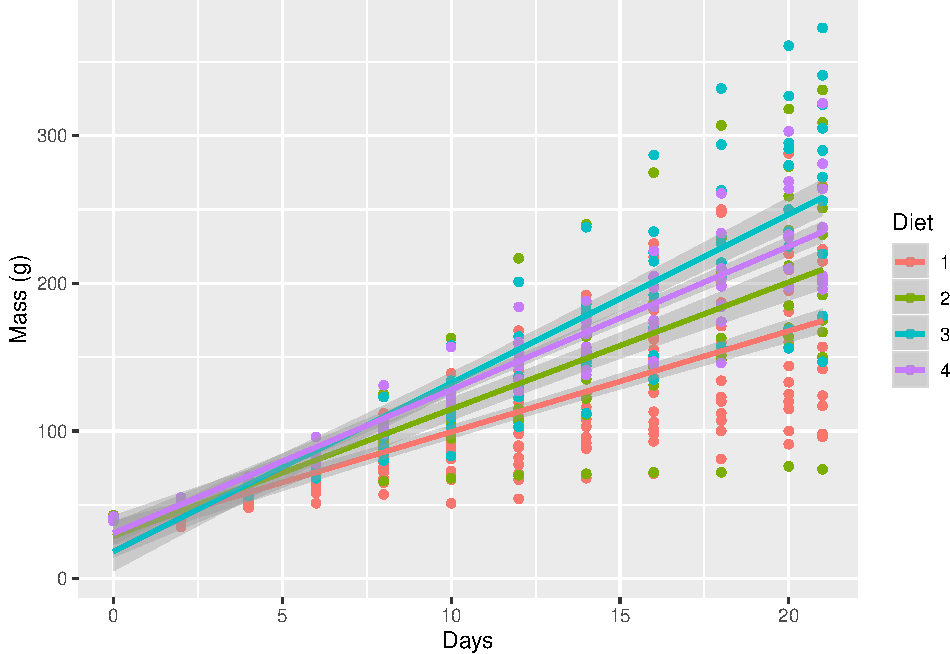
\includegraphics{06-faceting_files/figure-latex/facet-lm-1.pdf}
\caption{\label{fig:facet-lm}Linear models for the progression of chicken weights (g) over time (days) based on four different diets.}
\end{figure}

\hypertarget{histogram}{%
\subsection{Histogram}\label{histogram}}

\begin{Shaded}
\begin{Highlighting}[]
\CommentTok{\# Note that we are using \textquotesingle{}ChickLast\textquotesingle{}, not \textquotesingle{}ChickWeight\textquotesingle{}}
\NormalTok{histogram\_}\DecValTok{1}\NormalTok{ <{-}}\StringTok{ }\KeywordTok{ggplot}\NormalTok{(}\DataTypeTok{data =}\NormalTok{ ChickLast, }\KeywordTok{aes}\NormalTok{(}\DataTypeTok{x =}\NormalTok{ weight)) }\OperatorTok{+}
\StringTok{  }\KeywordTok{geom\_histogram}\NormalTok{(}\KeywordTok{aes}\NormalTok{(}\DataTypeTok{fill =}\NormalTok{ Diet), }\DataTypeTok{position =} \StringTok{"dodge"}\NormalTok{, }\DataTypeTok{binwidth =} \DecValTok{100}\NormalTok{) }\OperatorTok{+}
\StringTok{  }\KeywordTok{labs}\NormalTok{(}\DataTypeTok{x =} \StringTok{"Final Mass (g)"}\NormalTok{, }\DataTypeTok{y =} \StringTok{"Count"}\NormalTok{)}
\NormalTok{histogram\_}\DecValTok{1}
\end{Highlighting}
\end{Shaded}

\begin{figure}
\centering
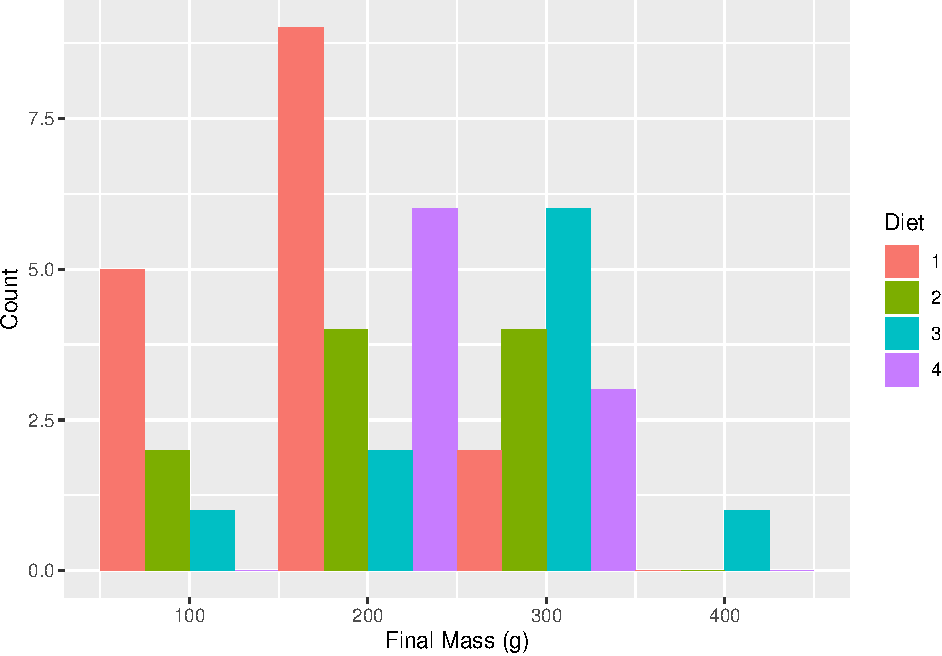
\includegraphics{06-faceting_files/figure-latex/facet-hist-1.pdf}
\caption{\label{fig:facet-hist}Histogram showing final chicken weights (g) by diet.}
\end{figure}

\hypertarget{boxplot}{%
\subsection{Boxplot}\label{boxplot}}

\begin{Shaded}
\begin{Highlighting}[]
\CommentTok{\# Note that we are using \textquotesingle{}ChickLast\textquotesingle{}, not \textquotesingle{}ChickWeight\textquotesingle{}}
\NormalTok{box\_}\DecValTok{1}\NormalTok{ <{-}}\StringTok{ }\KeywordTok{ggplot}\NormalTok{(}\DataTypeTok{data =}\NormalTok{ ChickLast, }\KeywordTok{aes}\NormalTok{(}\DataTypeTok{x =}\NormalTok{ Diet, }\DataTypeTok{y =}\NormalTok{ weight)) }\OperatorTok{+}
\StringTok{  }\KeywordTok{geom\_boxplot}\NormalTok{(}\KeywordTok{aes}\NormalTok{(}\DataTypeTok{fill =}\NormalTok{ Diet)) }\OperatorTok{+}
\StringTok{  }\KeywordTok{labs}\NormalTok{(}\DataTypeTok{x =} \StringTok{"Diet"}\NormalTok{, }\DataTypeTok{y =} \StringTok{"Final Mass (g)"}\NormalTok{)}
\NormalTok{box\_}\DecValTok{1}
\end{Highlighting}
\end{Shaded}

\begin{figure}
\centering
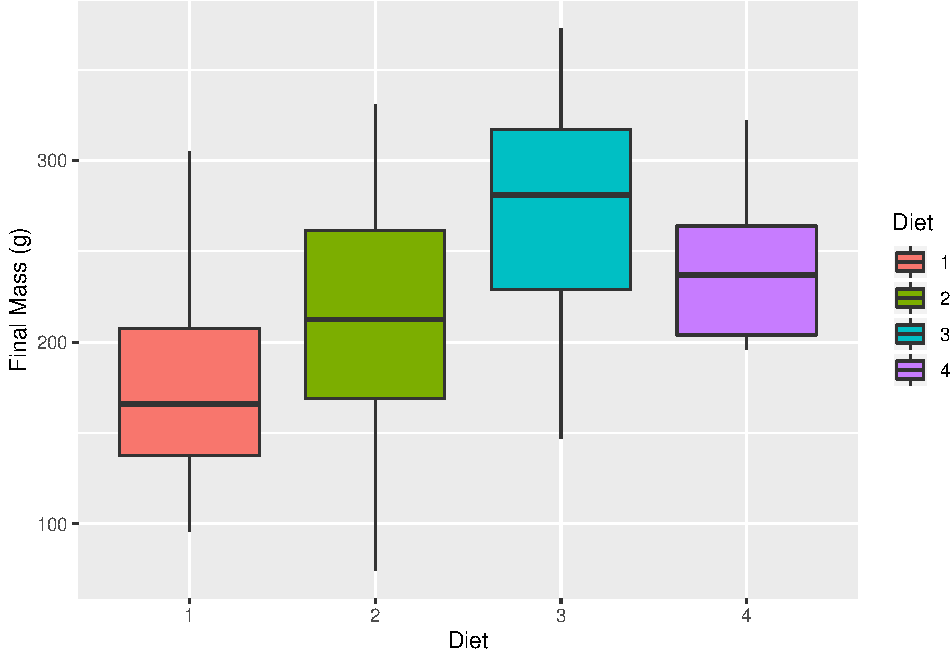
\includegraphics{06-faceting_files/figure-latex/facet-box-1.pdf}
\caption{\label{fig:facet-box}Violin plot showing the distribution of final chicken weights (g) by diet.}
\end{figure}

\hypertarget{gridding-figures}{%
\section{Gridding figures}\label{gridding-figures}}

With these four different figures created we may now look at how to combine them. By visualising the data in different ways they are able to tell us different parts of the same story. What do we see from the figures below that we may not have seen when looking at each figure individually?

\begin{Shaded}
\begin{Highlighting}[]
\KeywordTok{ggarrange}\NormalTok{(line\_}\DecValTok{1}\NormalTok{, lm\_}\DecValTok{1}\NormalTok{, histogram\_}\DecValTok{1}\NormalTok{, box\_}\DecValTok{1}\NormalTok{, }
          \DataTypeTok{ncol =} \DecValTok{2}\NormalTok{, }\DataTypeTok{nrow =} \DecValTok{2}\NormalTok{, }\CommentTok{\# Set number of rows and columns}
          \DataTypeTok{labels =} \KeywordTok{c}\NormalTok{(}\StringTok{"A"}\NormalTok{, }\StringTok{"B"}\NormalTok{, }\StringTok{"C"}\NormalTok{, }\StringTok{"D"}\NormalTok{), }\CommentTok{\# Label each figure}
          \DataTypeTok{common.legend =} \OtherTok{TRUE}\NormalTok{) }\CommentTok{\# Create common legend}
\end{Highlighting}
\end{Shaded}

\begin{figure}
\centering
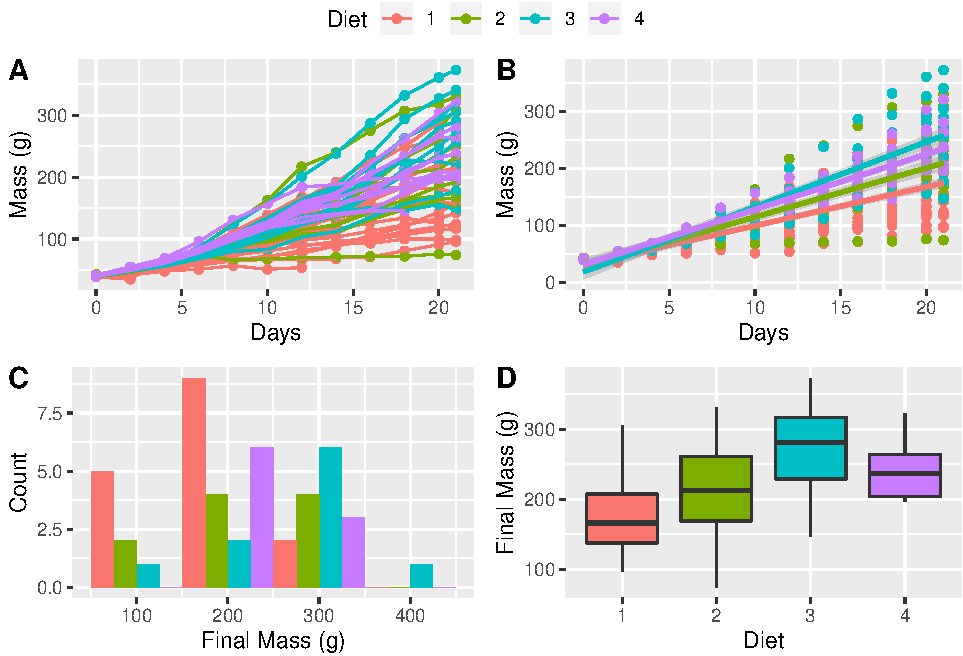
\includegraphics{06-faceting_files/figure-latex/facet-grid-1.pdf}
\caption{\label{fig:facet-grid}All four of our figures gridded together with an automagically created common legend.}
\end{figure}

The above figure looks great, so let's save a copy of it as a PDF to our computer. In order to do so we will need to assign our figure to an object and then use the \texttt{ggsave()} function on that object.

\begin{Shaded}
\begin{Highlighting}[]
\CommentTok{\# First we must assign the code to an object name}
\NormalTok{grid\_}\DecValTok{1}\NormalTok{ <{-}}\StringTok{ }\KeywordTok{ggarrange}\NormalTok{(lm\_}\DecValTok{1}\NormalTok{, histogram\_}\DecValTok{1}\NormalTok{, density\_}\DecValTok{1}\NormalTok{, violin\_}\DecValTok{1}\NormalTok{, }
                    \DataTypeTok{ncol =} \DecValTok{2}\NormalTok{, }\DataTypeTok{nrow =} \DecValTok{2}\NormalTok{, }
                    \DataTypeTok{labels =} \KeywordTok{c}\NormalTok{(}\StringTok{"A"}\NormalTok{, }\StringTok{"B"}\NormalTok{, }\StringTok{"C"}\NormalTok{, }\StringTok{"D"}\NormalTok{),}
                    \DataTypeTok{common.legend =} \OtherTok{TRUE}\NormalTok{)}

\CommentTok{\# Then we save the object we created}
\KeywordTok{ggsave}\NormalTok{(}\DataTypeTok{plot =}\NormalTok{ grid\_}\DecValTok{1}\NormalTok{, }\DataTypeTok{filename =} \StringTok{"figures/grid\_1.pdf"}\NormalTok{)}
\end{Highlighting}
\end{Shaded}

\hypertarget{session-info-4}{%
\section{Session info}\label{session-info-4}}

\begin{Shaded}
\begin{Highlighting}[]
\KeywordTok{installed.packages}\NormalTok{()[}\KeywordTok{names}\NormalTok{(}\KeywordTok{sessionInfo}\NormalTok{()}\OperatorTok{$}\NormalTok{otherPkgs), }\StringTok{"Version"}\NormalTok{]}
\end{Highlighting}
\end{Shaded}

\begin{verbatim}
R>    ggpubr  magrittr   forcats   stringr     dplyr     purrr     readr     tidyr 
R>   "0.2.4"     "1.5"   "0.4.0"   "1.4.0"   "0.8.3"   "0.3.3"   "1.3.1"   "1.0.0" 
R>    tibble   ggplot2 tidyverse 
R>   "2.1.3"   "3.2.1"   "1.3.0"
\end{verbatim}

\hypertarget{brewing}{%
\chapter{\texorpdfstring{Brewing colours in \textbf{\texttt{ggplot2}}}{Brewing colours in ggplot2}}\label{brewing}}

\begin{quote}
``Every portrait that is painted with feeling is a portrait of the artist, not of the sitter.''

--- Oscar Wilde
\end{quote}

\begin{quote}
``If you could say it in words, there would be no reason to paint.''

--- Edward Hopper
\end{quote}

Now that we have seen the basics of \textbf{\texttt{ggplot2}}, let's take a moment to delve further into the beauty of our figures. It may sound vain at first, but the colour palette of a figure is actually very important. This is for two main reasons. The first being that a consistent colour palette looks more professional. But most importantly it is necessary to have a good colour palette because it makes the information in our figures easier to understand. The communication of information to others is central to good science.

\hypertarget{r-data}{%
\section{R Data}\label{r-data}}

Before we get going on our figures, we first need to learn more about the built in data that R has. The base R program that we all have loaded on our computers already comes with heaps of example dataframes that we may use for practice. We don't need to load our own data. Additionally, whenever we install a new package (and by now we've already installed dozens) it usually comes with several new dataframes. There are many ways to look at the data that we have available from our packages. Below we show two of the many options.

\begin{Shaded}
\begin{Highlighting}[]
\CommentTok{\# To create a list of ALL available data}
  \CommentTok{\# Not really recommended as the output is overwhelming}
\KeywordTok{data}\NormalTok{(}\DataTypeTok{package =} \KeywordTok{.packages}\NormalTok{(}\DataTypeTok{all.available =} \OtherTok{TRUE}\NormalTok{))}

\CommentTok{\# To look for datasets within a single known package}
  \CommentTok{\# type the name of the package followed by \textquotesingle{}::\textquotesingle{}}
  \CommentTok{\# This tells R you want to look in the specified package}
  \CommentTok{\# When the autocomplete bubble comes up you may scroll}
  \CommentTok{\# through it with the up and down arrows}
  \CommentTok{\# Look for objects that have a mini spreadsheet icon}
  \CommentTok{\# These are the datasets}

\CommentTok{\# Try typing the following code and see what happens...}
\NormalTok{datasets}\OperatorTok{::}
\end{Highlighting}
\end{Shaded}

We have an amazing amount of data available to us. So the challenge is not to find a dataframe that works for us, but to just decide on one. My preferred method is to read the short descriptions of the dataframes and pick the one that sounds the funniest. But please use whatever method makes the most sense to you. One note of caution, in R there are generally two different forms of data: wide OR long. We will see in detail what this means on Day 4, and what to do about it. For now we just need to know that \textbf{\texttt{ggplot2}} works much better with long data. To look at a dataframe of interest we use the same method we would use to look up a help file for a function.

Over the years I've installed so many packages on my computer that it is difficult to chose a dataframe. The package \textbf{\texttt{boot}} has some particularly interesting dataframes with a biological focus. Please install this now to access to these data. I have decided to load the \texttt{urine} dataframe here. Note that \texttt{library(boot)} will not work on your computer if you have not installed the package yet. With these data we will now make a scatterplot with two of the variables, while changing the colour of the dots with a third variable.

\begin{Shaded}
\begin{Highlighting}[]
\CommentTok{\# Load libraries}
\KeywordTok{library}\NormalTok{(tidyverse)}
\KeywordTok{library}\NormalTok{(boot)}

\CommentTok{\# Load data}
\NormalTok{urine <{-}}\StringTok{ }\NormalTok{boot}\OperatorTok{::}\NormalTok{urine}

\CommentTok{\# Look at help file for more info}
\CommentTok{\# ?urine}

\CommentTok{\# Create a quick scatterplot}
\KeywordTok{ggplot}\NormalTok{(}\DataTypeTok{data =}\NormalTok{ urine, }\KeywordTok{aes}\NormalTok{(}\DataTypeTok{x =}\NormalTok{ osmo, }\DataTypeTok{y =}\NormalTok{ ph)) }\OperatorTok{+}
\StringTok{  }\KeywordTok{geom\_point}\NormalTok{(}\KeywordTok{aes}\NormalTok{(}\DataTypeTok{colour =}\NormalTok{ cond))}
\end{Highlighting}
\end{Shaded}

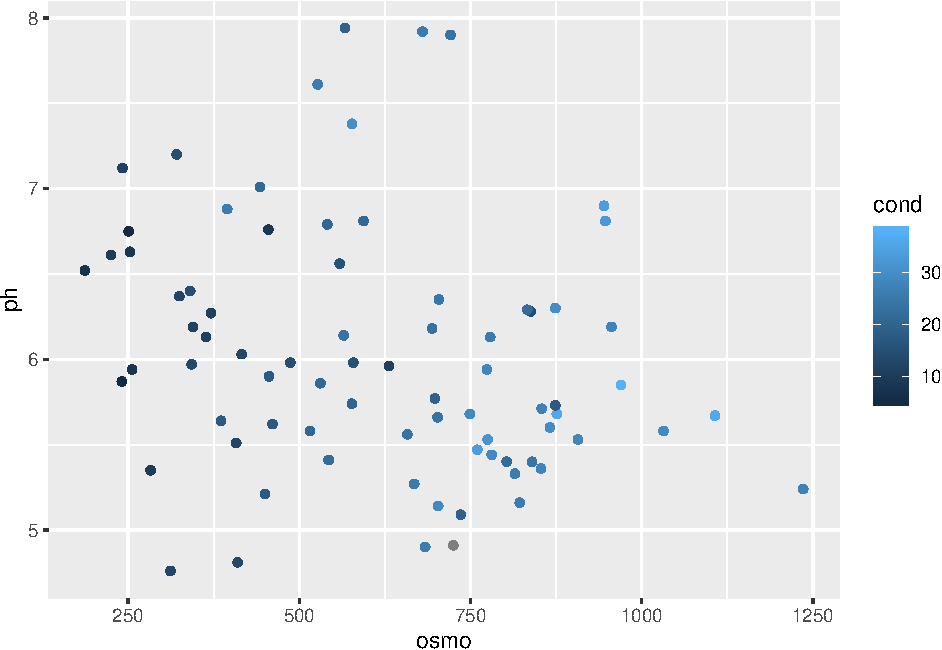
\includegraphics{07-brewing_files/figure-latex/brew-1-1.pdf}

And now we have a scatterplot that is showing the relationship between the osmolarity and pH of urine, with the conductivity of those urine samples shown in shades of blue. What is important to note here is that the colour scale is continuous. How can we now this by looking at the figure? Let's look at the same figure but use a discrete variable for colouring.

\begin{Shaded}
\begin{Highlighting}[]
\KeywordTok{ggplot}\NormalTok{(}\DataTypeTok{data =}\NormalTok{ urine, }\KeywordTok{aes}\NormalTok{(}\DataTypeTok{x =}\NormalTok{ osmo, }\DataTypeTok{y =}\NormalTok{ ph)) }\OperatorTok{+}
\StringTok{  }\KeywordTok{geom\_point}\NormalTok{(}\KeywordTok{aes}\NormalTok{(}\DataTypeTok{colour =} \KeywordTok{as.factor}\NormalTok{(r)))}
\end{Highlighting}
\end{Shaded}

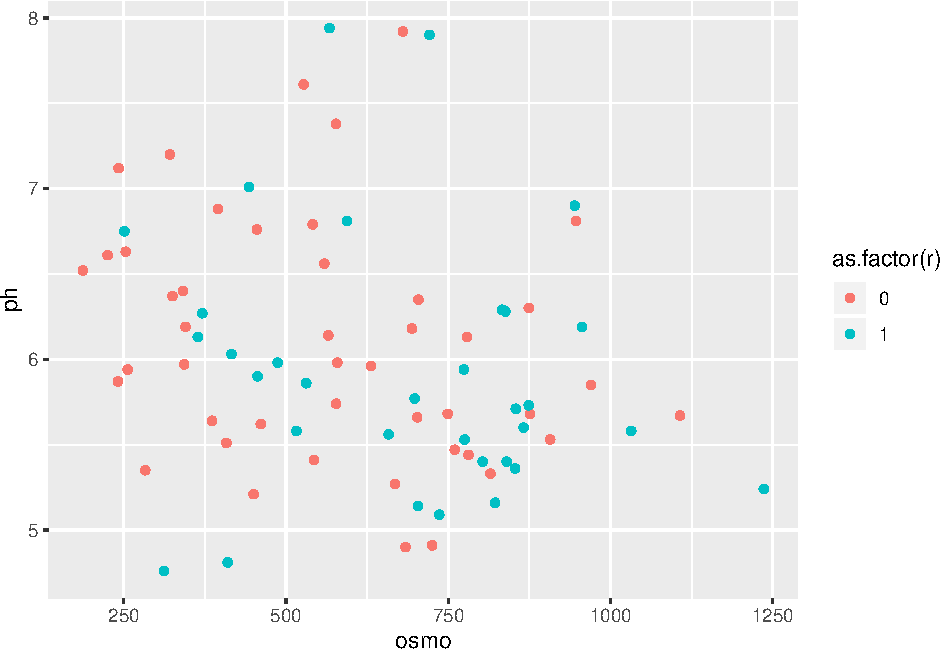
\includegraphics{07-brewing_files/figure-latex/brew-2-1.pdf}

What is the first thing you notice about the difference in the colours? Why did we use \texttt{as.factor()} for the colour aesthetic for our points? What happens if we don't use this? Try it now.

\hypertarget{rcolorbrewer}{%
\section{\texorpdfstring{\textbf{\texttt{RColorBrewer}}}{RColorBrewer}}\label{rcolorbrewer}}

Central to the purpose of \textbf{\texttt{ggplot2}} is the creation of beautiful figures. For this reason there are many built in functions that we may use in order to have precise control over the colours we use, as well as additional packages that extend our options even further. The \textbf{\texttt{RColorBrewer}} package should have been installed on your computer and activated automatically when we installed and activated the \textbf{\texttt{tidyverse}}. We will use this package for its lovely colour palettes. Let's spruce up the previous continuous colour scale figure now.

\begin{Shaded}
\begin{Highlighting}[]
\CommentTok{\# The continuous colour scale figure}
\KeywordTok{ggplot}\NormalTok{(}\DataTypeTok{data =}\NormalTok{ urine, }\KeywordTok{aes}\NormalTok{(}\DataTypeTok{x =}\NormalTok{ osmo, }\DataTypeTok{y =}\NormalTok{ ph)) }\OperatorTok{+}
\StringTok{  }\KeywordTok{geom\_point}\NormalTok{(}\KeywordTok{aes}\NormalTok{(}\DataTypeTok{colour =}\NormalTok{ cond)) }\OperatorTok{+}
\StringTok{  }\KeywordTok{scale\_colour\_distiller}\NormalTok{() }\CommentTok{\# Change the continuous variable colour palette}
\end{Highlighting}
\end{Shaded}

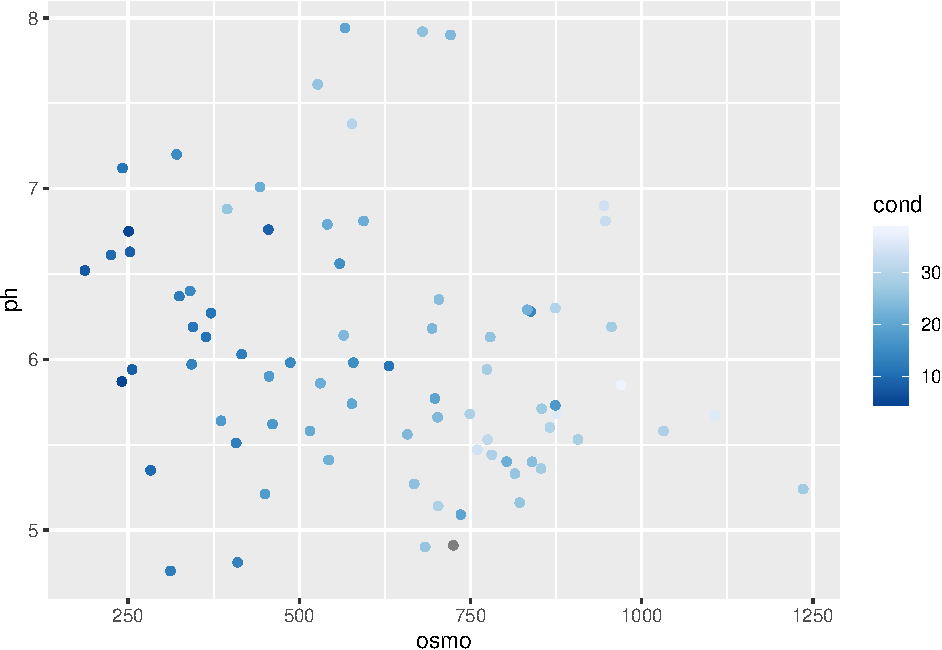
\includegraphics{07-brewing_files/figure-latex/brew-3-1.pdf}

Does this look different? If so, how? The second page of the colour cheat sheet we included in the course material shows some different colour brewer palettes. Let's look at how to use those here.

\begin{Shaded}
\begin{Highlighting}[]
\KeywordTok{ggplot}\NormalTok{(}\DataTypeTok{data =}\NormalTok{ urine, }\KeywordTok{aes}\NormalTok{(}\DataTypeTok{x =}\NormalTok{ osmo, }\DataTypeTok{y =}\NormalTok{ ph)) }\OperatorTok{+}
\StringTok{  }\KeywordTok{geom\_point}\NormalTok{(}\KeywordTok{aes}\NormalTok{(}\DataTypeTok{colour =}\NormalTok{ cond)) }\OperatorTok{+}
\StringTok{  }\KeywordTok{scale\_colour\_distiller}\NormalTok{(}\DataTypeTok{palette =} \StringTok{"Spectral"}\NormalTok{)}
\end{Highlighting}
\end{Shaded}

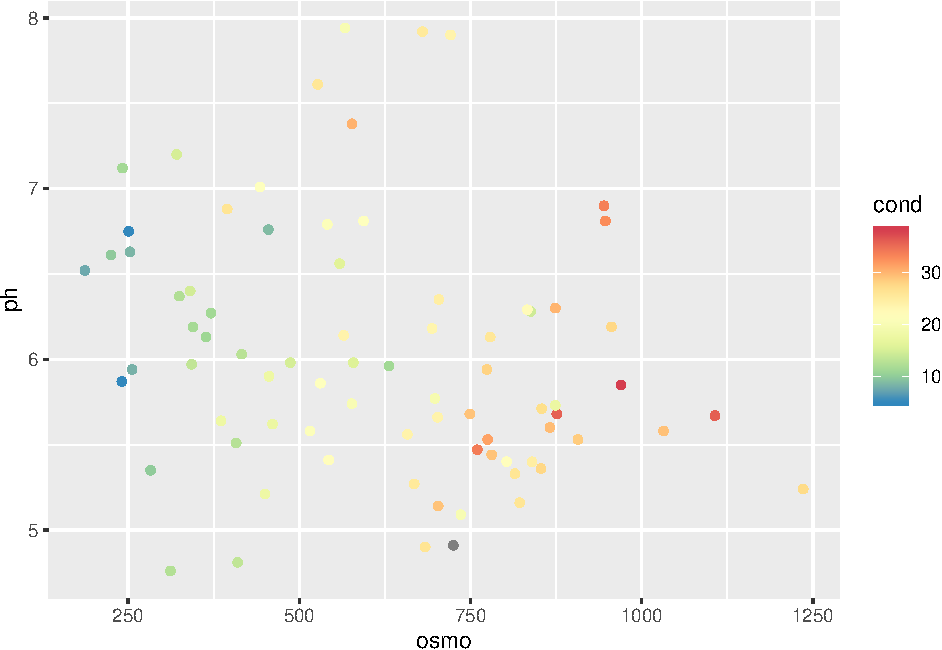
\includegraphics{07-brewing_files/figure-latex/brew-4-1.pdf}

Does that help us to see a pattern in the data? What do we see? Does it look like there are any significant relationships here? How would we test that?

If we want to use colour brewer with a discrete variable we use a slightly different function.

\begin{Shaded}
\begin{Highlighting}[]
\KeywordTok{ggplot}\NormalTok{(}\DataTypeTok{data =}\NormalTok{ urine, }\KeywordTok{aes}\NormalTok{(}\DataTypeTok{x =}\NormalTok{ osmo, }\DataTypeTok{y =}\NormalTok{ ph)) }\OperatorTok{+}
\StringTok{  }\KeywordTok{geom\_point}\NormalTok{(}\KeywordTok{aes}\NormalTok{(}\DataTypeTok{colour =} \KeywordTok{as.factor}\NormalTok{(r))) }\OperatorTok{+}
\StringTok{  }\KeywordTok{scale\_colour\_brewer}\NormalTok{() }\CommentTok{\# This is the different function}
\end{Highlighting}
\end{Shaded}

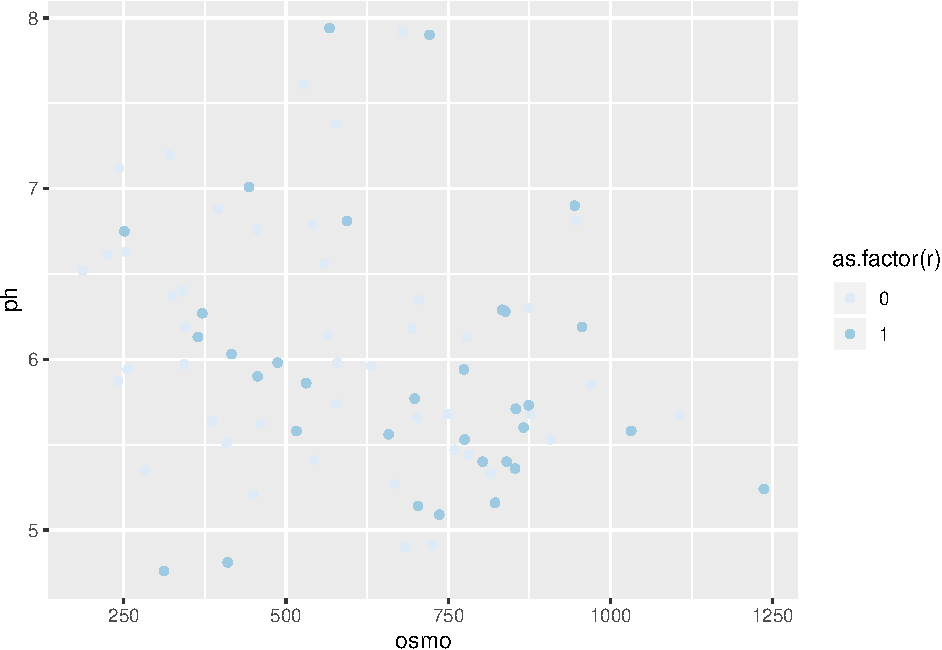
\includegraphics{07-brewing_files/figure-latex/brew-5-1.pdf}

The default colour scale here is not helpful at all. So let's pick a better one. If we look at our cheat sheet we will see a list of different continuous and discrete colour scales. All we need to do is copy and paste one of these names into our colour brewer function with inverted commas.

\begin{Shaded}
\begin{Highlighting}[]
\KeywordTok{ggplot}\NormalTok{(}\DataTypeTok{data =}\NormalTok{ urine, }\KeywordTok{aes}\NormalTok{(}\DataTypeTok{x =}\NormalTok{ osmo, }\DataTypeTok{y =}\NormalTok{ ph)) }\OperatorTok{+}
\StringTok{  }\KeywordTok{geom\_point}\NormalTok{(}\KeywordTok{aes}\NormalTok{(}\DataTypeTok{colour =} \KeywordTok{as.factor}\NormalTok{(r))) }\OperatorTok{+}
\StringTok{  }\KeywordTok{scale\_colour\_brewer}\NormalTok{(}\DataTypeTok{palette =} \StringTok{"Set1"}\NormalTok{) }\CommentTok{\# Here I used "Set1", but use what you like}
\end{Highlighting}
\end{Shaded}

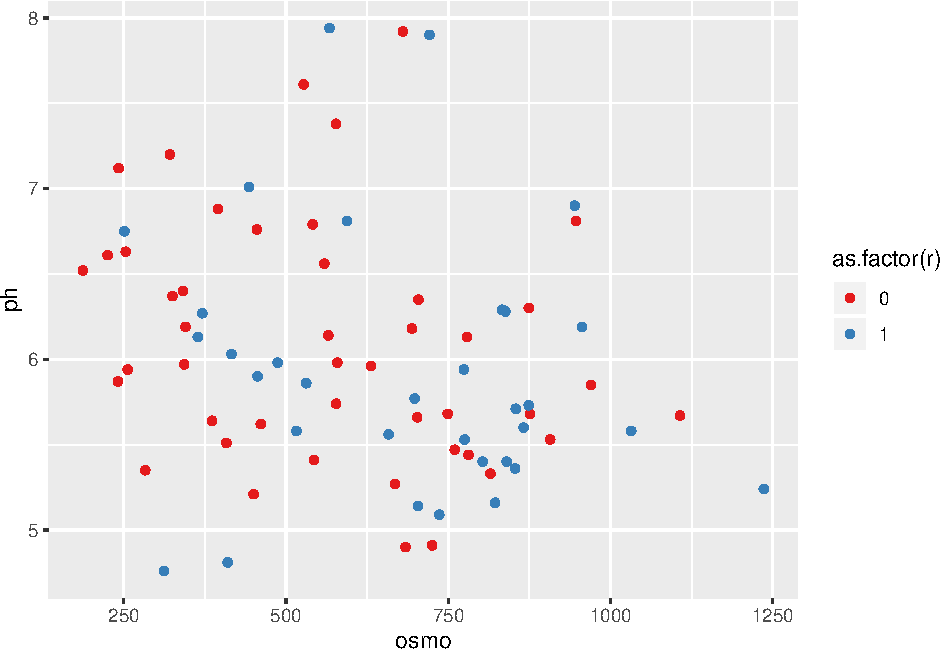
\includegraphics{07-brewing_files/figure-latex/brew-6-1.pdf}

\hypertarget{make-your-own-palettes}{%
\section{Make your own palettes}\label{make-your-own-palettes}}

This is all well and good. But didn't we claim that this should give us complete control over our colours? So far it looks like it has just given us a few more palettes to use. And that's nice, but it's not `infinite choices'. That is where the Internet comes to our rescue. There are many places we may go to for support in this regard. The following links, in descending order, are very useful. And fun!

\begin{itemize}
\tightlist
\item
  \url{http://tristen.ca/hcl-picker/\#/hlc/6/0.95/48B4B6/345363}
\item
  \url{http://tools.medialab.sciences-po.fr/iwanthue/index.php}
\item
  \url{http://jsfiddle.net/d6wXV/6/embedded/result/}
\end{itemize}

I find the first link the easiest to use. But the second and third links are better at generating discrete colour palettes. Take several minutes playing with the different websites and decide for yourself which one(s) you like.

\hypertarget{use-your-own-palettes}{%
\section{Use your own palettes}\label{use-your-own-palettes}}

Now that we've had some time to play around with the colour generators let's look at how to use them with our figures. I've used the first web link to create a list of five colours. I then copy and pasted them into the code below, separating them with commas and placing them inside of \texttt{c()} and inverted commas. Be certain that you insert commas and inverted commas as necessary or you will get errors. Note also that we are using a new function to use our custom palette.

\begin{Shaded}
\begin{Highlighting}[]
\KeywordTok{ggplot}\NormalTok{(}\DataTypeTok{data =}\NormalTok{ urine, }\KeywordTok{aes}\NormalTok{(}\DataTypeTok{x =}\NormalTok{ osmo, }\DataTypeTok{y =}\NormalTok{ ph)) }\OperatorTok{+}
\StringTok{  }\KeywordTok{geom\_point}\NormalTok{(}\KeywordTok{aes}\NormalTok{(}\DataTypeTok{colour =}\NormalTok{ cond)) }\OperatorTok{+}
\StringTok{  }\KeywordTok{scale\_colour\_gradientn}\NormalTok{(}\DataTypeTok{colours =} \KeywordTok{c}\NormalTok{(}\StringTok{"\#A5A94D"}\NormalTok{, }\StringTok{"\#6FB16F"}\NormalTok{, }\StringTok{"\#45B19B"}\NormalTok{,}
                                    \StringTok{"\#59A9BE"}\NormalTok{, }\StringTok{"\#9699C4"}\NormalTok{, }\StringTok{"\#CA86AD"}\NormalTok{))}
\end{Highlighting}
\end{Shaded}

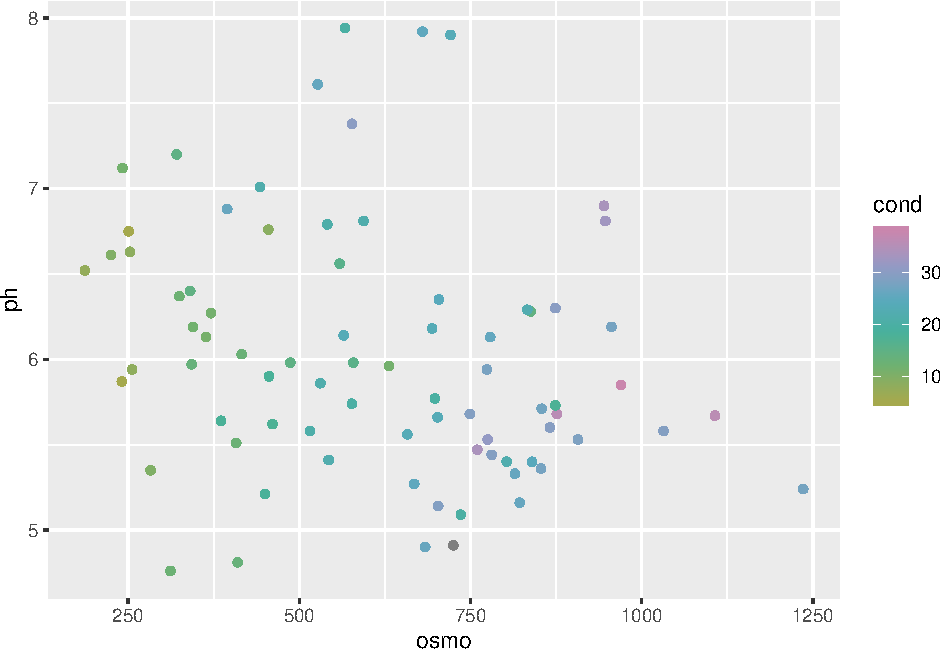
\includegraphics{07-brewing_files/figure-latex/brew-7-1.pdf}

If we want to use our custom colour palettes with a discrete colour scale we use a different function as seen in the code below. While we are at it, let's also see how to correct the title of the legend and its text labels. Sometimes the default output is not what we want for our final figure. Especially if we are going to be publishing it. Also note in the following code chunk that rather than using hexadecimal character strings to represent colours in our custom palette, we are simply writing in the human name for the colours we want. This will work for the continuous colour palettes above, too.

\begin{Shaded}
\begin{Highlighting}[]
\KeywordTok{ggplot}\NormalTok{(}\DataTypeTok{data =}\NormalTok{ urine, }\KeywordTok{aes}\NormalTok{(}\DataTypeTok{x =}\NormalTok{ osmo, }\DataTypeTok{y =}\NormalTok{ ph)) }\OperatorTok{+}
\StringTok{  }\KeywordTok{geom\_point}\NormalTok{(}\KeywordTok{aes}\NormalTok{(}\DataTypeTok{colour =} \KeywordTok{as.factor}\NormalTok{(r))) }\OperatorTok{+}
\StringTok{  }\KeywordTok{scale\_colour\_manual}\NormalTok{(}\DataTypeTok{values =} \KeywordTok{c}\NormalTok{(}\StringTok{"pink"}\NormalTok{, }\StringTok{"maroon"}\NormalTok{), }\CommentTok{\# How to use custom palette}
                     \DataTypeTok{labels =} \KeywordTok{c}\NormalTok{(}\StringTok{"no"}\NormalTok{, }\StringTok{"yes"}\NormalTok{)) }\OperatorTok{+}\StringTok{ }\CommentTok{\# How to change the legend text}
\StringTok{  }\KeywordTok{labs}\NormalTok{(}\DataTypeTok{colour =} \StringTok{"crystals"}\NormalTok{) }\CommentTok{\# How to change the legend title}
\end{Highlighting}
\end{Shaded}

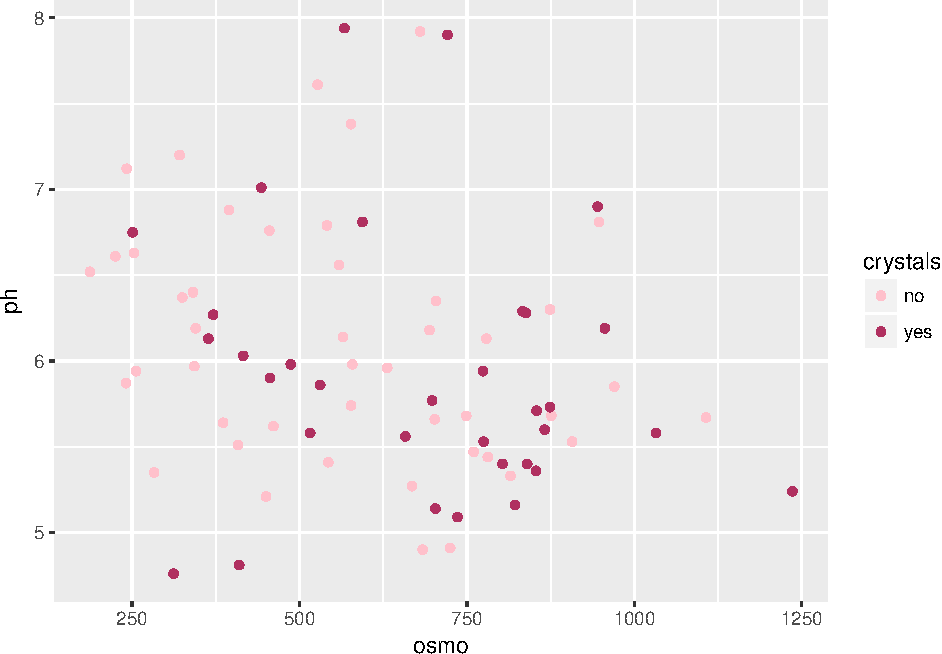
\includegraphics{07-brewing_files/figure-latex/brew-8-1.pdf}

So now we have seen how to control the colours palettes in our figures. I know it is a but much. Four new functions just to change some colours! That's a bummer. Don't forget that one of the main benefits of R is that all of your code is written down, annotated and saved. You don't need to remember which button to click to change the colours, you just need to remember where you saved the code that you will need. And that's pretty great in my opinion.

\hypertarget{diy-figures}{%
\section{DIY figures}\label{diy-figures}}

Today we learned the basics of \textbf{\texttt{ggplot2}}, how to facet, how to brew colours, and how to plot stats. Sjog, that's a lot of stuff to remember! Which is why we will now spend the rest of Day 2 putting our new found skills to use. Please group up as you see fit to produce your very own \textbf{\texttt{ggplot2}} figures. We've not yet learned how to manipulate/tidy up our data so it may be challenging to grab any ol' dataset and make a plan with it. To that end we recommend using the \texttt{laminaria} or \texttt{ecklonia} datasets we saw on Day 1. You are of course free to use whatever dataset you would like, including your own. The goal by the end of today is to have created at least two figures (first prize for four figures) and join them together via faceting. We will be walking the room to help with any issues that may arise.

\hypertarget{session-info-5}{%
\section{Session info}\label{session-info-5}}

\begin{Shaded}
\begin{Highlighting}[]
\KeywordTok{installed.packages}\NormalTok{()[}\KeywordTok{names}\NormalTok{(}\KeywordTok{sessionInfo}\NormalTok{()}\OperatorTok{$}\NormalTok{otherPkgs), }\StringTok{"Version"}\NormalTok{]}
\end{Highlighting}
\end{Shaded}

\begin{verbatim}
R>      boot   forcats   stringr     dplyr     purrr     readr     tidyr    tibble 
R>  "1.3-24"   "0.4.0"   "1.4.0"   "0.8.3"   "0.3.3"   "1.3.1"   "1.0.0"   "2.1.3" 
R>   ggplot2 tidyverse 
R>   "3.2.1"   "1.3.0"
\end{verbatim}

\hypertarget{mapping}{%
\chapter{\texorpdfstring{Mapping with \textbf{\texttt{ggplot2}}}{Mapping with ggplot2}}\label{mapping}}

\begin{quote}
``There's no map to human behaviour.''

--- Bjork
\end{quote}

\begin{quote}
``Here be dragons''

--- Unknown
\end{quote}

Yesterday we learned how to create \textbf{\texttt{ggplot2}} figures, change their aesthetics, labels, colour palettes, and facet/arrange them. Now we are going to look at how to create maps.

Most of the work that we perform as environmental/biological scientists involves going out to a location and sampling information there. Sometimes only once, and sometimes over a period of time. All of these different sampling methods lend themselves to different types of figures. One of those, collection of data at different points, is best shown with maps. As we will see over the course of Day 3, creating maps in \textbf{\texttt{ggplot2}} is very straight forward and is extensively supported. For that reason we are going to have plenty of time to also learn how to do some more advanced things. Our goal in this chapter is to produce the figure below.

\begin{figure}

{\centering 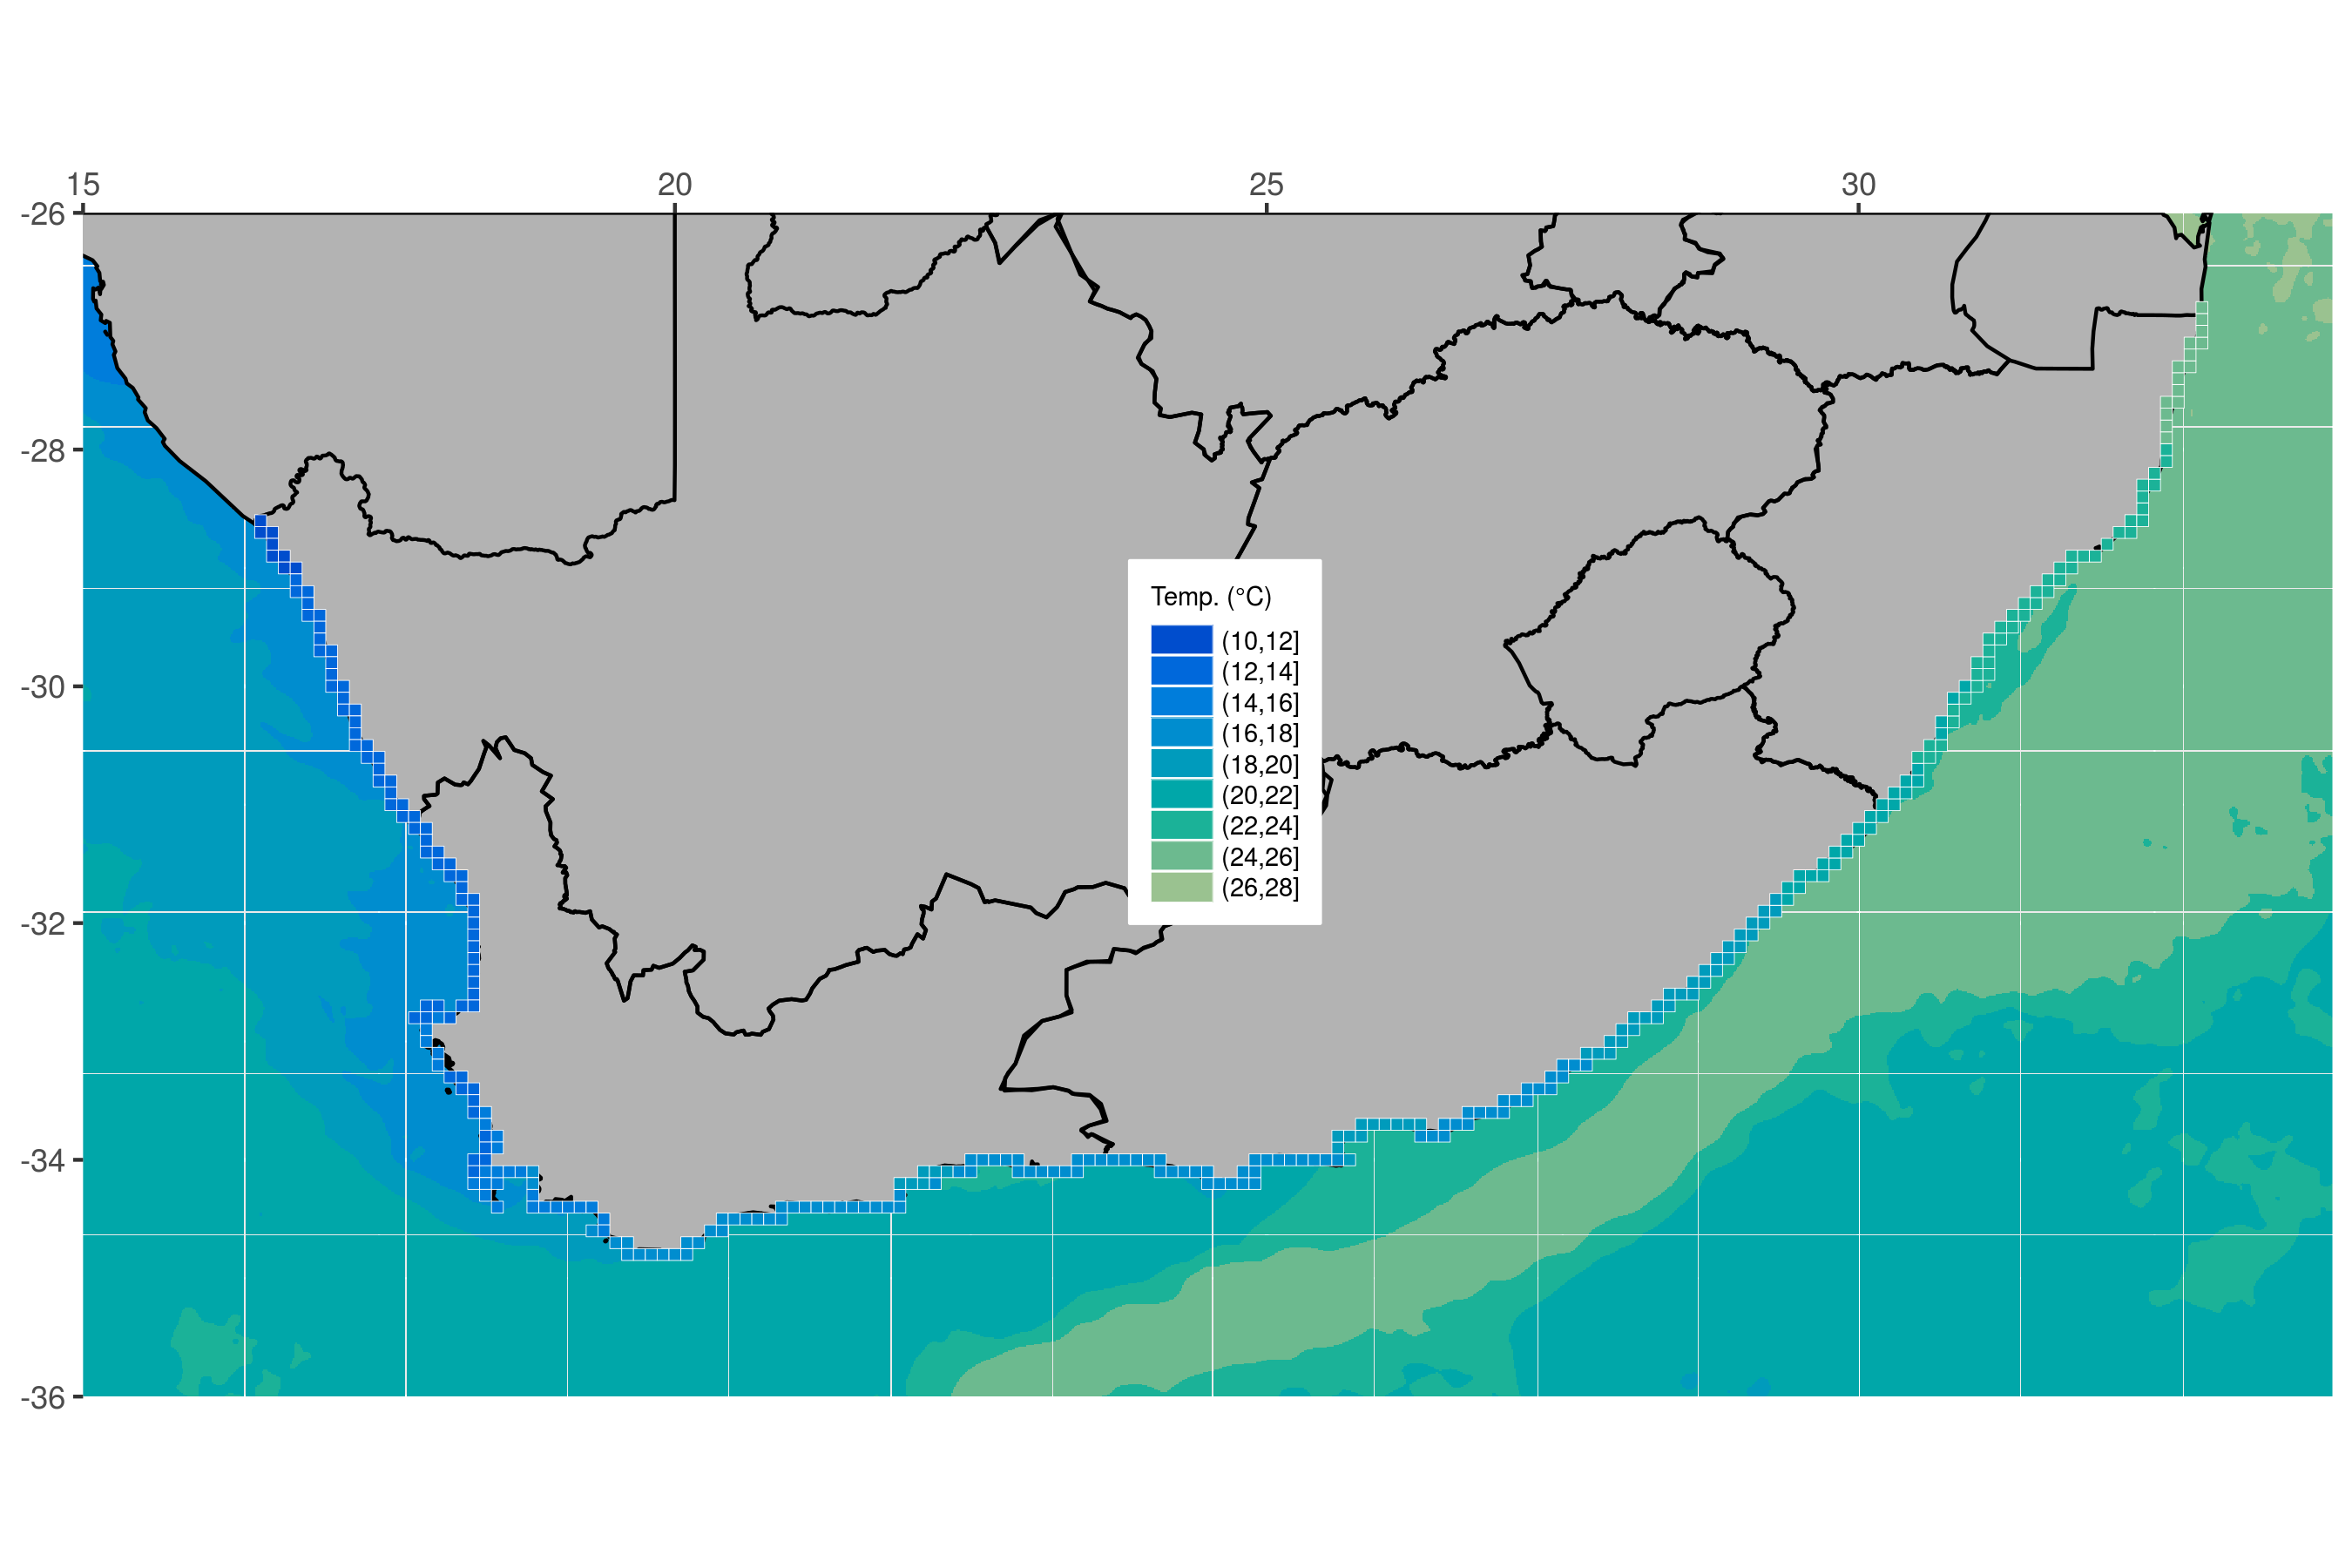
\includegraphics[width=1\linewidth]{figures/map_complete} 

}

\caption{The goal for today.}\label{fig:map-goal}
\end{figure}

Before we begin let's go ahead and load the packages we will need, as well as the several dataframes required to make the final product.

\begin{Shaded}
\begin{Highlighting}[]
\CommentTok{\# Load libraries}
\KeywordTok{library}\NormalTok{(tidyverse)}
\KeywordTok{library}\NormalTok{(ggpubr)}

\CommentTok{\# Load data}
\KeywordTok{load}\NormalTok{(}\StringTok{"data/south\_africa\_coast.RData"}\NormalTok{)}
\KeywordTok{load}\NormalTok{(}\StringTok{"data/sa\_provinces.RData"}\NormalTok{)}
\KeywordTok{load}\NormalTok{(}\StringTok{"data/rast\_annual.RData"}\NormalTok{)}
\KeywordTok{load}\NormalTok{(}\StringTok{"data/MUR.RData"}\NormalTok{)}
\KeywordTok{load}\NormalTok{(}\StringTok{"data/MUR\_low\_res.RData"}\NormalTok{)}

\CommentTok{\# Choose which SST product you would like to use}
\NormalTok{sst <{-}}\StringTok{ }\NormalTok{MUR\_low\_res}
\CommentTok{\# OR}
\NormalTok{sst <{-}}\StringTok{ }\NormalTok{MUR}

\CommentTok{\# The colour pallette we will use for ocean temperature}
\NormalTok{cols11 <{-}}\StringTok{ }\KeywordTok{c}\NormalTok{(}\StringTok{"\#004dcd"}\NormalTok{, }\StringTok{"\#0068db"}\NormalTok{, }\StringTok{"\#007ddb"}\NormalTok{, }\StringTok{"\#008dcf"}\NormalTok{, }\StringTok{"\#009bbc"}\NormalTok{,}
            \StringTok{"\#00a7a9"}\NormalTok{, }\StringTok{"\#1bb298"}\NormalTok{, }\StringTok{"\#6cba8f"}\NormalTok{, }\StringTok{"\#9ac290"}\NormalTok{, }\StringTok{"\#bec99a"}\NormalTok{)}
\end{Highlighting}
\end{Shaded}

\hypertarget{a-new-concept}{%
\section{A new concept?}\label{a-new-concept}}

The idea of creating a map in R may be daunting to some, but remember that a basic map is nothing more than a simple figure with an x and y axis. We tend to think of maps as different from other scientific figures, whereas in reality they are created the exact same way. Let's compare a dot plot of the chicken weight data against a dot plot of the coastline of South Africa.

Chicken dots:

\begin{Shaded}
\begin{Highlighting}[]
\KeywordTok{ggplot}\NormalTok{(}\DataTypeTok{data =}\NormalTok{ ChickWeight, }\KeywordTok{aes}\NormalTok{(}\DataTypeTok{x =}\NormalTok{ Time, }\DataTypeTok{y =}\NormalTok{ weight)) }\OperatorTok{+}
\StringTok{  }\KeywordTok{geom\_point}\NormalTok{()}
\end{Highlighting}
\end{Shaded}

\begin{figure}
\centering
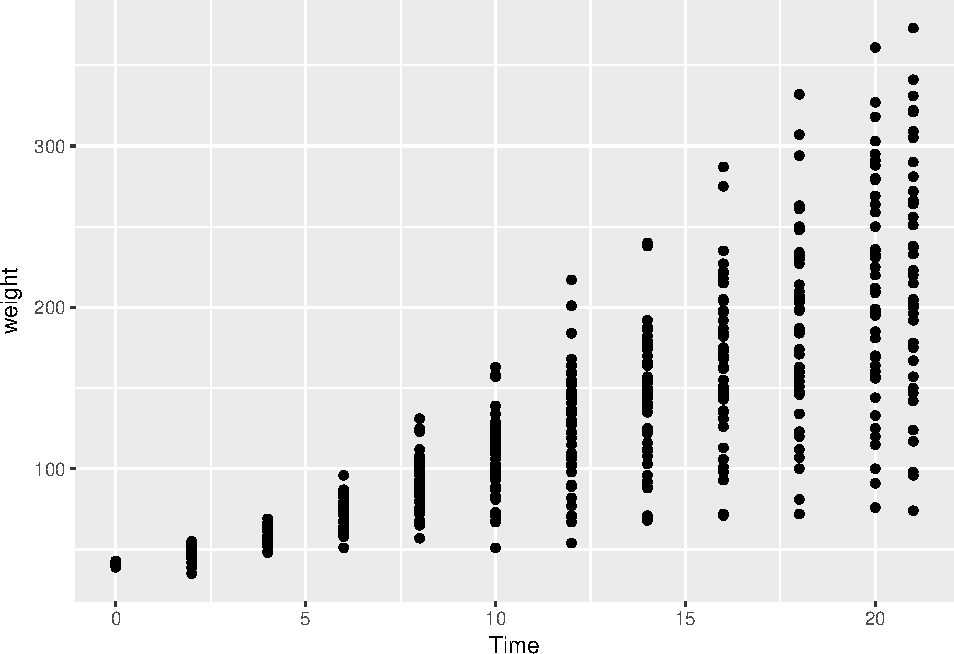
\includegraphics{08-mapping_files/figure-latex/map-point-1-1.pdf}
\caption{\label{fig:map-point-1}Dot plot of chicken weight data.}
\end{figure}

South African coast dots:

\begin{Shaded}
\begin{Highlighting}[]
\KeywordTok{ggplot}\NormalTok{(}\DataTypeTok{data =}\NormalTok{ south\_africa\_coast, }\KeywordTok{aes}\NormalTok{(}\DataTypeTok{x =}\NormalTok{ lon, }\DataTypeTok{y =}\NormalTok{ lat)) }\OperatorTok{+}
\StringTok{  }\KeywordTok{geom\_point}\NormalTok{()}
\end{Highlighting}
\end{Shaded}

\begin{figure}
\centering
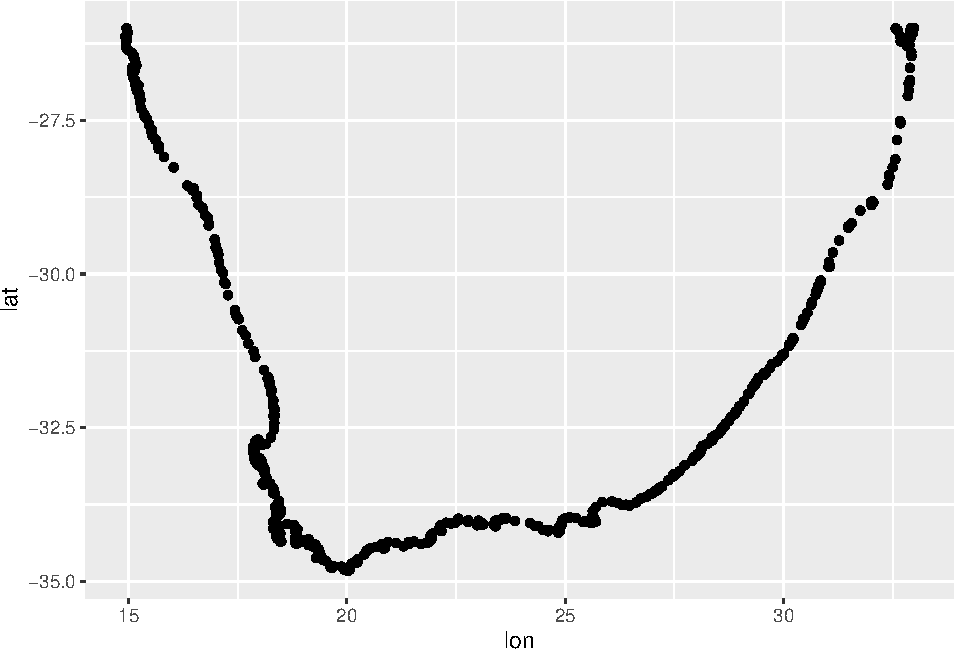
\includegraphics{08-mapping_files/figure-latex/map-point-2-1.pdf}
\caption{\label{fig:map-point-2}Dot plot off South African coast.}
\end{figure}

Does that look familiar? Notice how the x and y axis tick labels look the same as any map you would see in an atlas. This is because they are. But this isn't a great way to create a map. Rather it is better to represent the land mass with a polygon. With \textbf{\texttt{ggplot2}} this is a simple task.

\hypertarget{land-mask}{%
\section{Land mask}\label{land-mask}}

Now that we have seen that a map is nothing more than a bunch of dots and shapes on specific points along the x and y axes we are going to look at the steps we would take to build a more complex map. Don't worry if this seems daunting at first. We are going to take this step by step and ensure that each step is made clear along the way. The first step is to create a polygon. Note that we create an aesthetic argument inside of \texttt{geom\_polygon()} and not \texttt{ggplot()} because some of the steps we will take later on will not accept the \texttt{group} aesthetic. Remember, whatever aesthetic arguments we put inside of \texttt{ggplot()} will be inserted for us into all of our other \texttt{geom\_...()} lines of code.

\begin{Shaded}
\begin{Highlighting}[]
\KeywordTok{ggplot}\NormalTok{(}\DataTypeTok{data =}\NormalTok{ south\_africa\_coast, }\KeywordTok{aes}\NormalTok{(}\DataTypeTok{x =}\NormalTok{ lon, }\DataTypeTok{y =}\NormalTok{ lat)) }\OperatorTok{+}
\StringTok{  }\KeywordTok{geom\_polygon}\NormalTok{(}\DataTypeTok{colour =} \StringTok{"black"}\NormalTok{, }\DataTypeTok{fill =} \StringTok{"grey70"}\NormalTok{, }\KeywordTok{aes}\NormalTok{(}\DataTypeTok{group =}\NormalTok{ group)) }\CommentTok{\# The land mask}
\end{Highlighting}
\end{Shaded}

\begin{figure}
\centering
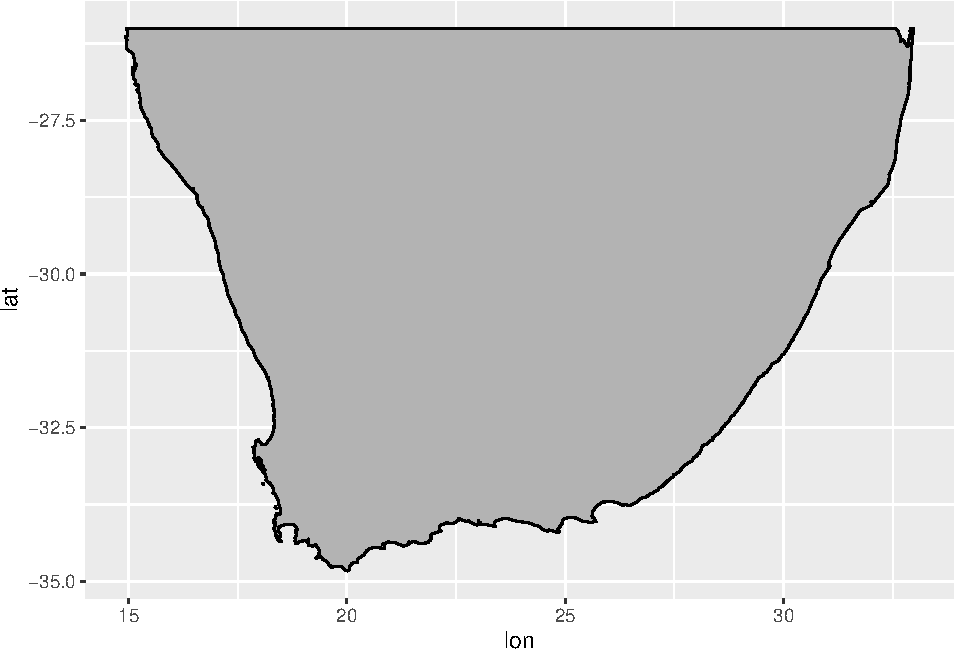
\includegraphics{08-mapping_files/figure-latex/map-polygon-1.pdf}
\caption{\label{fig:map-polygon}The map of South Africa. Now with province borders!}
\end{figure}

\hypertarget{borders}{%
\section{Borders}\label{borders}}

The first thing we will add is the province borders as seen in Figure \ref{fig:map-goal}. Notice how we only add one more line of code to do this.

\begin{Shaded}
\begin{Highlighting}[]
\KeywordTok{ggplot}\NormalTok{(}\DataTypeTok{data =}\NormalTok{ south\_africa\_coast, }\KeywordTok{aes}\NormalTok{(}\DataTypeTok{x =}\NormalTok{ lon, }\DataTypeTok{y =}\NormalTok{ lat)) }\OperatorTok{+}
\StringTok{  }\KeywordTok{geom\_polygon}\NormalTok{(}\DataTypeTok{colour =} \StringTok{"black"}\NormalTok{, }\DataTypeTok{fill =} \StringTok{"grey70"}\NormalTok{, }\KeywordTok{aes}\NormalTok{(}\DataTypeTok{group =}\NormalTok{ group)) }\OperatorTok{+}
\StringTok{  }\KeywordTok{geom\_path}\NormalTok{(}\DataTypeTok{data =}\NormalTok{ sa\_provinces, }\KeywordTok{aes}\NormalTok{(}\DataTypeTok{group =}\NormalTok{ group)) }\CommentTok{\# The province borders}
\end{Highlighting}
\end{Shaded}

\begin{figure}
\centering
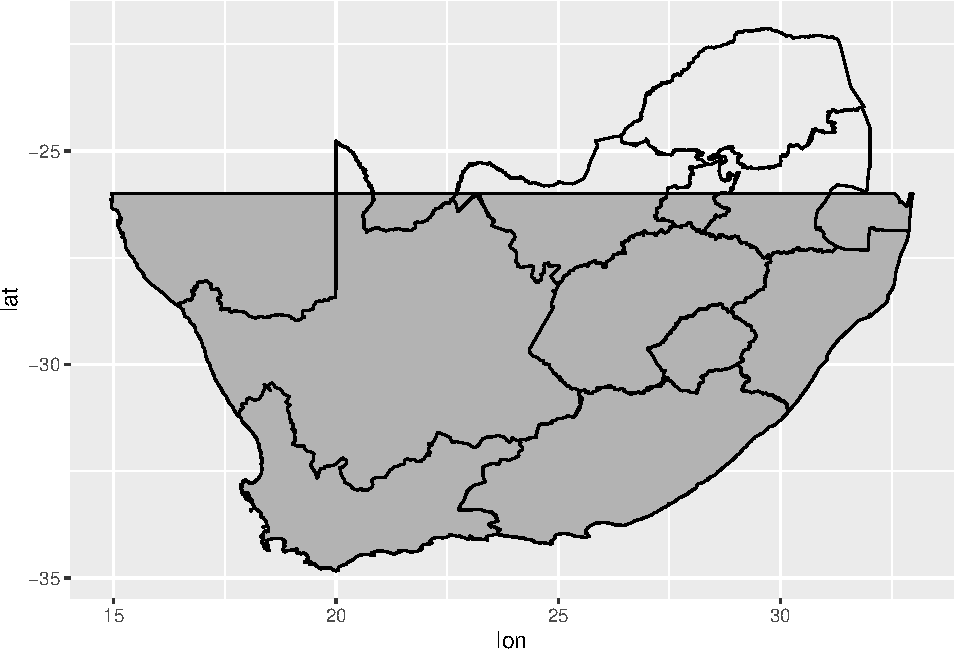
\includegraphics{08-mapping_files/figure-latex/map-province-1.pdf}
\caption{\label{fig:map-province}The map of South Africa. Now with province borders!}
\end{figure}

\hypertarget{force-lonlat-extent}{%
\section{Force lon/lat extent}\label{force-lonlat-extent}}

Unfortunately when we added our borders it increased the plotting area of our map past what we would like. To correct that we will need to explicitly state the borders we want.

\begin{Shaded}
\begin{Highlighting}[]
\KeywordTok{ggplot}\NormalTok{(}\DataTypeTok{data =}\NormalTok{ south\_africa\_coast, }\KeywordTok{aes}\NormalTok{(}\DataTypeTok{x =}\NormalTok{ lon, }\DataTypeTok{y =}\NormalTok{ lat)) }\OperatorTok{+}
\StringTok{  }\KeywordTok{geom\_polygon}\NormalTok{(}\DataTypeTok{colour =} \StringTok{"black"}\NormalTok{, }\DataTypeTok{fill =} \StringTok{"grey70"}\NormalTok{, }\KeywordTok{aes}\NormalTok{(}\DataTypeTok{group =}\NormalTok{ group)) }\OperatorTok{+}
\StringTok{  }\KeywordTok{geom\_path}\NormalTok{(}\DataTypeTok{data =}\NormalTok{ sa\_provinces, }\KeywordTok{aes}\NormalTok{(}\DataTypeTok{group =}\NormalTok{ group)) }\OperatorTok{+}\StringTok{ }
\StringTok{  }\KeywordTok{coord\_equal}\NormalTok{(}\DataTypeTok{xlim =} \KeywordTok{c}\NormalTok{(}\DecValTok{15}\NormalTok{, }\DecValTok{34}\NormalTok{), }\DataTypeTok{ylim =} \KeywordTok{c}\NormalTok{(}\OperatorTok{{-}}\DecValTok{36}\NormalTok{, }\DecValTok{{-}26}\NormalTok{), }\DataTypeTok{expand =} \DecValTok{0}\NormalTok{) }\CommentTok{\# Force lon/lat extent}
\end{Highlighting}
\end{Shaded}

\begin{figure}
\centering
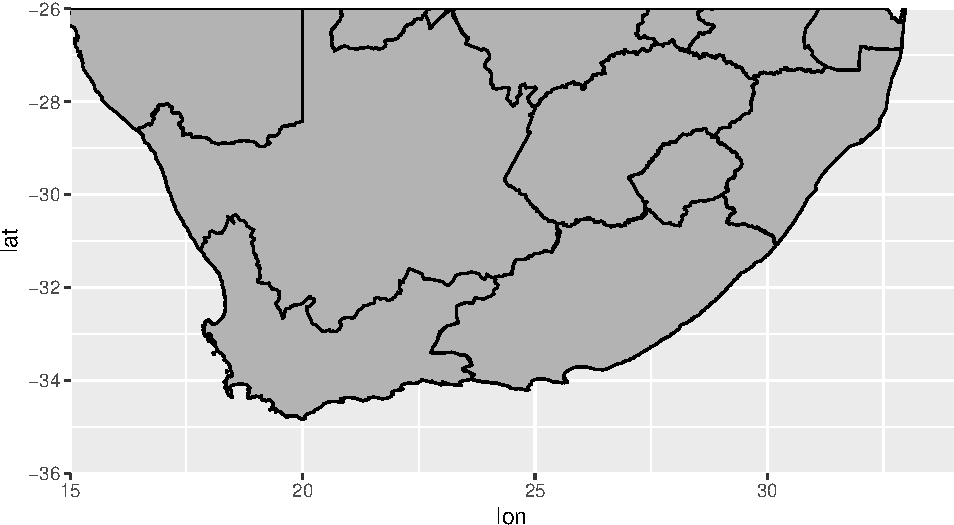
\includegraphics{08-mapping_files/figure-latex/map-expand-1.pdf}
\caption{\label{fig:map-expand}The map, but with the extra bits snipped off.}
\end{figure}

\hypertarget{ocean-temperature}{%
\section{Ocean temperature}\label{ocean-temperature}}

This is starting to look pretty fancy, but it would be nicer if there was some colour involved. So let's add the ocean temperature. Again, this will only require one more line of code. Starting to see a pattern? But what is different this time and why?

\begin{Shaded}
\begin{Highlighting}[]
\KeywordTok{ggplot}\NormalTok{(}\DataTypeTok{data =}\NormalTok{ south\_africa\_coast, }\KeywordTok{aes}\NormalTok{(}\DataTypeTok{x =}\NormalTok{ lon, }\DataTypeTok{y =}\NormalTok{ lat)) }\OperatorTok{+}
\StringTok{  }\KeywordTok{geom\_raster}\NormalTok{(}\DataTypeTok{data =}\NormalTok{ sst, }\KeywordTok{aes}\NormalTok{(}\DataTypeTok{fill =}\NormalTok{ bins)) }\OperatorTok{+}\StringTok{ }\CommentTok{\# The ocean temperatures}
\StringTok{  }\KeywordTok{geom\_polygon}\NormalTok{(}\DataTypeTok{colour =} \StringTok{"black"}\NormalTok{, }\DataTypeTok{fill =} \StringTok{"grey70"}\NormalTok{, }\KeywordTok{aes}\NormalTok{(}\DataTypeTok{group =}\NormalTok{ group)) }\OperatorTok{+}
\StringTok{  }\KeywordTok{geom\_path}\NormalTok{(}\DataTypeTok{data =}\NormalTok{ sa\_provinces, }\KeywordTok{aes}\NormalTok{(}\DataTypeTok{group =}\NormalTok{ group)) }\OperatorTok{+}
\StringTok{  }\KeywordTok{coord\_equal}\NormalTok{(}\DataTypeTok{xlim =} \KeywordTok{c}\NormalTok{(}\DecValTok{15}\NormalTok{, }\DecValTok{34}\NormalTok{), }\DataTypeTok{ylim =} \KeywordTok{c}\NormalTok{(}\OperatorTok{{-}}\DecValTok{36}\NormalTok{, }\DecValTok{{-}26}\NormalTok{), }\DataTypeTok{expand =} \DecValTok{0}\NormalTok{)}
\end{Highlighting}
\end{Shaded}

\begin{figure}
\centering
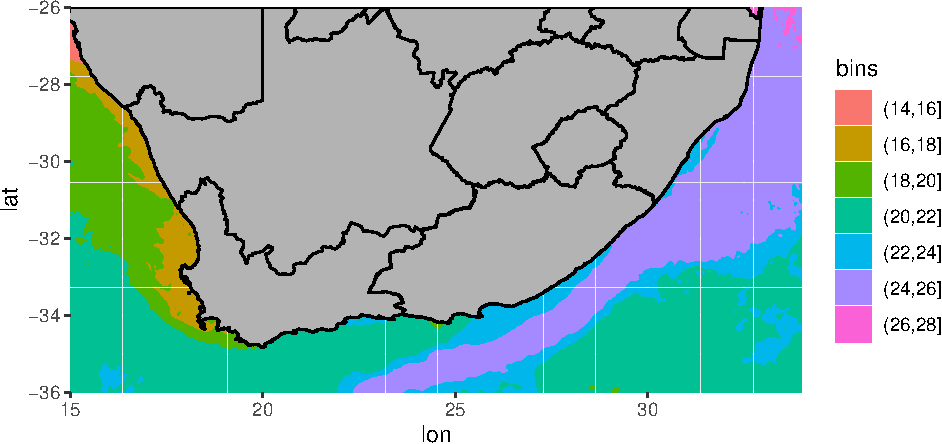
\includegraphics{08-mapping_files/figure-latex/map-MUR-1.pdf}
\caption{\label{fig:map-MUR}Ocean temperature (°C) visualised as an ice cream spill.}
\end{figure}

That looks\ldots{} odd. Why do the colours look like someone melted a big bucket of ice cream in the ocean? This is because the colours you see in this figure are the default colours for discrete values in \textbf{\texttt{ggplot2}}. If we want to change them we may do so easily by adding yet one more line of code.

\begin{Shaded}
\begin{Highlighting}[]
\KeywordTok{ggplot}\NormalTok{(}\DataTypeTok{data =}\NormalTok{ south\_africa\_coast, }\KeywordTok{aes}\NormalTok{(}\DataTypeTok{x =}\NormalTok{ lon, }\DataTypeTok{y =}\NormalTok{ lat)) }\OperatorTok{+}
\StringTok{  }\KeywordTok{geom\_raster}\NormalTok{(}\DataTypeTok{data =}\NormalTok{ sst, }\KeywordTok{aes}\NormalTok{(}\DataTypeTok{fill =}\NormalTok{ bins)) }\OperatorTok{+}
\StringTok{  }\KeywordTok{geom\_polygon}\NormalTok{(}\DataTypeTok{colour =} \StringTok{"black"}\NormalTok{, }\DataTypeTok{fill =} \StringTok{"grey70"}\NormalTok{, }\KeywordTok{aes}\NormalTok{(}\DataTypeTok{group =}\NormalTok{ group)) }\OperatorTok{+}
\StringTok{  }\KeywordTok{geom\_path}\NormalTok{(}\DataTypeTok{data =}\NormalTok{ sa\_provinces, }\KeywordTok{aes}\NormalTok{(}\DataTypeTok{group =}\NormalTok{ group)) }\OperatorTok{+}
\StringTok{  }\KeywordTok{scale\_fill\_manual}\NormalTok{(}\StringTok{"Temp. (°C)"}\NormalTok{, }\DataTypeTok{values =}\NormalTok{ cols11) }\OperatorTok{+}\StringTok{ }\CommentTok{\# Set the colour palette}
\StringTok{  }\KeywordTok{coord\_equal}\NormalTok{(}\DataTypeTok{xlim =} \KeywordTok{c}\NormalTok{(}\DecValTok{15}\NormalTok{, }\DecValTok{34}\NormalTok{), }\DataTypeTok{ylim =} \KeywordTok{c}\NormalTok{(}\OperatorTok{{-}}\DecValTok{36}\NormalTok{, }\DecValTok{{-}26}\NormalTok{), }\DataTypeTok{expand =} \DecValTok{0}\NormalTok{)}
\end{Highlighting}
\end{Shaded}

\begin{figure}
\centering
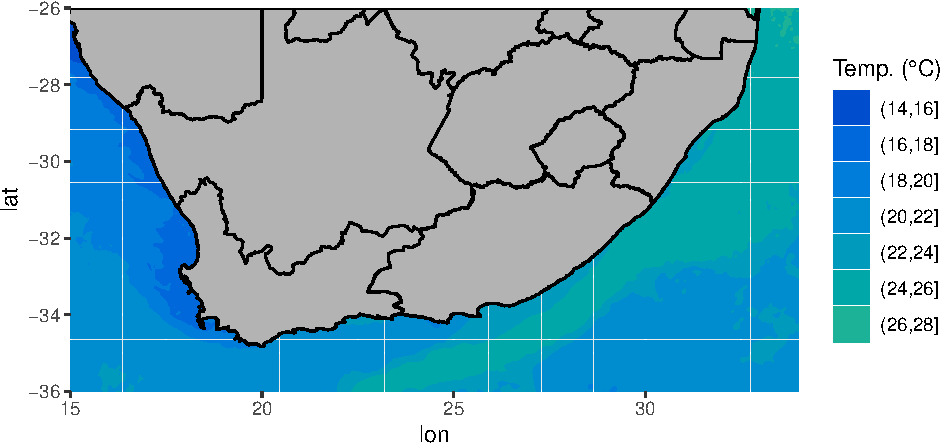
\includegraphics{08-mapping_files/figure-latex/map-colour-1.pdf}
\caption{\label{fig:map-colour}Ocean temperatures (°C) around South Africa.}
\end{figure}

There's a colour palette that would make Jacques Cousteau swoon. When we set the colour palette for a figure in \textbf{\texttt{ggplot2}} we must use that colour palette for all other instances of those types of values, too. What this means is that any other discrete values that will be filled in, like the ocean colour above, must use the same colour palette (there are some technical exceptions to this rule that we will not cover in this course). We normally want \textbf{\texttt{ggplot2}} to use consistent colour palettes anyway, but it is important to note that this constraint exists. Let's see what we mean. Next we will add the coastal pixels to our figure with one more line of code. We won't change anything else. Note how \textbf{\texttt{ggplot2}} changes the colour of the coastal pixels to match the ocean colour automatically.

\begin{Shaded}
\begin{Highlighting}[]
\KeywordTok{ggplot}\NormalTok{(}\DataTypeTok{data =}\NormalTok{ south\_africa\_coast, }\KeywordTok{aes}\NormalTok{(}\DataTypeTok{x =}\NormalTok{ lon, }\DataTypeTok{y =}\NormalTok{ lat)) }\OperatorTok{+}
\StringTok{  }\KeywordTok{geom\_raster}\NormalTok{(}\DataTypeTok{data =}\NormalTok{ sst, }\KeywordTok{aes}\NormalTok{(}\DataTypeTok{fill =}\NormalTok{ bins)) }\OperatorTok{+}
\StringTok{  }\KeywordTok{geom\_polygon}\NormalTok{(}\DataTypeTok{colour =} \StringTok{"black"}\NormalTok{, }\DataTypeTok{fill =} \StringTok{"grey70"}\NormalTok{, }\KeywordTok{aes}\NormalTok{(}\DataTypeTok{group =}\NormalTok{ group)) }\OperatorTok{+}
\StringTok{  }\KeywordTok{geom\_path}\NormalTok{(}\DataTypeTok{data =}\NormalTok{ sa\_provinces, }\KeywordTok{aes}\NormalTok{(}\DataTypeTok{group =}\NormalTok{ group)) }\OperatorTok{+}
\StringTok{  }\KeywordTok{geom\_tile}\NormalTok{(}\DataTypeTok{data =}\NormalTok{ rast\_annual, }\KeywordTok{aes}\NormalTok{(}\DataTypeTok{x =}\NormalTok{ lon, }\DataTypeTok{y =}\NormalTok{ lat, }\DataTypeTok{fill =}\NormalTok{ bins), }
            \DataTypeTok{colour =} \StringTok{"white"}\NormalTok{, }\DataTypeTok{size =} \FloatTok{0.1}\NormalTok{) }\OperatorTok{+}\StringTok{ }\CommentTok{\# The coastal temperature values}
\StringTok{  }\KeywordTok{scale\_fill\_manual}\NormalTok{(}\StringTok{"Temp. (°C)"}\NormalTok{, }\DataTypeTok{values =}\NormalTok{ cols11) }\OperatorTok{+}
\StringTok{  }\KeywordTok{coord\_equal}\NormalTok{(}\DataTypeTok{xlim =} \KeywordTok{c}\NormalTok{(}\DecValTok{15}\NormalTok{, }\DecValTok{34}\NormalTok{), }\DataTypeTok{ylim =} \KeywordTok{c}\NormalTok{(}\OperatorTok{{-}}\DecValTok{36}\NormalTok{, }\DecValTok{{-}26}\NormalTok{), }\DataTypeTok{expand =} \DecValTok{0}\NormalTok{)}
\end{Highlighting}
\end{Shaded}

\begin{figure}
\centering
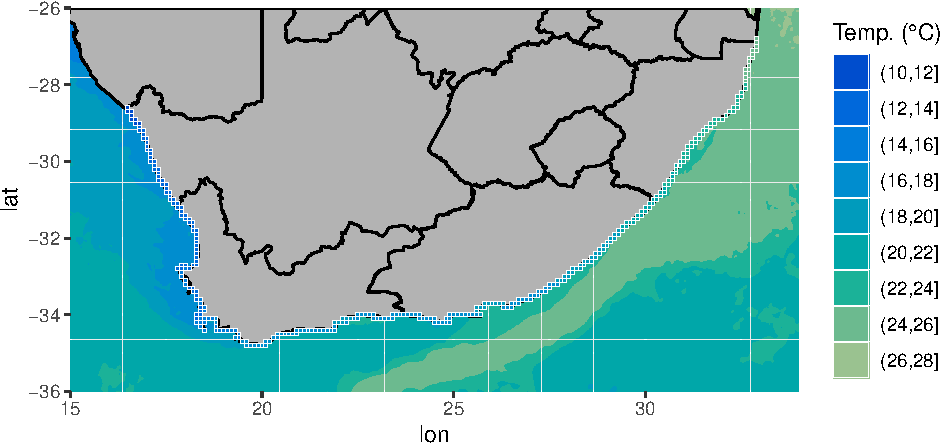
\includegraphics{08-mapping_files/figure-latex/map-raster-1.pdf}
\caption{\label{fig:map-raster}Map of SOuth Africa showing \emph{in situ} temeperatures (°C) as pixels along the coast.}
\end{figure}

\hypertarget{final-touches}{%
\section{Final touches}\label{final-touches}}

We used \texttt{geom\_tile()} instead of \texttt{geom\_rast()} to add the coastal pixels above so that we could add those little white boxes around them. This figure is looking pretty great now. And it only took a few rows of code to put it all together! The last step is to add several more lines of code that will control for all of the little things we want to change about the appearance of the figure. Each little thing that is changed below is annotated for your convenience.

\begin{Shaded}
\begin{Highlighting}[]
\NormalTok{final\_map <{-}}\StringTok{ }\KeywordTok{ggplot}\NormalTok{(}\DataTypeTok{data =}\NormalTok{ south\_africa\_coast, }\KeywordTok{aes}\NormalTok{(}\DataTypeTok{x =}\NormalTok{ lon, }\DataTypeTok{y =}\NormalTok{ lat)) }\OperatorTok{+}
\StringTok{  }\KeywordTok{geom\_raster}\NormalTok{(}\DataTypeTok{data =}\NormalTok{ sst, }\KeywordTok{aes}\NormalTok{(}\DataTypeTok{fill =}\NormalTok{ bins)) }\OperatorTok{+}
\StringTok{  }\KeywordTok{geom\_polygon}\NormalTok{(}\DataTypeTok{colour =} \StringTok{"black"}\NormalTok{, }\DataTypeTok{fill =} \StringTok{"grey70"}\NormalTok{, }\KeywordTok{aes}\NormalTok{(}\DataTypeTok{group =}\NormalTok{ group)) }\OperatorTok{+}
\StringTok{  }\KeywordTok{geom\_path}\NormalTok{(}\DataTypeTok{data =}\NormalTok{ sa\_provinces, }\KeywordTok{aes}\NormalTok{(}\DataTypeTok{group =}\NormalTok{ group)) }\OperatorTok{+}
\StringTok{  }\KeywordTok{geom\_tile}\NormalTok{(}\DataTypeTok{data =}\NormalTok{ rast\_annual, }\KeywordTok{aes}\NormalTok{(}\DataTypeTok{x =}\NormalTok{ lon, }\DataTypeTok{y =}\NormalTok{ lat, }\DataTypeTok{fill =}\NormalTok{ bins), }
            \DataTypeTok{colour =} \StringTok{"white"}\NormalTok{, }\DataTypeTok{size =} \FloatTok{0.1}\NormalTok{) }\OperatorTok{+}
\StringTok{  }\KeywordTok{scale\_fill\_manual}\NormalTok{(}\StringTok{"Temp. (°C)"}\NormalTok{, }\DataTypeTok{values =}\NormalTok{ cols11) }\OperatorTok{+}
\StringTok{  }\KeywordTok{coord\_equal}\NormalTok{(}\DataTypeTok{xlim =} \KeywordTok{c}\NormalTok{(}\DecValTok{15}\NormalTok{, }\DecValTok{34}\NormalTok{), }\DataTypeTok{ylim =} \KeywordTok{c}\NormalTok{(}\OperatorTok{{-}}\DecValTok{36}\NormalTok{, }\DecValTok{{-}26}\NormalTok{), }\DataTypeTok{expand =} \DecValTok{0}\NormalTok{) }\OperatorTok{+}
\StringTok{  }\KeywordTok{scale\_x\_continuous}\NormalTok{(}\DataTypeTok{position =} \StringTok{"top"}\NormalTok{) }\OperatorTok{+}\StringTok{ }\CommentTok{\# Put x axis labels on top of figure}
\StringTok{  }\KeywordTok{theme}\NormalTok{(}\DataTypeTok{axis.title =} \KeywordTok{element\_blank}\NormalTok{(), }\CommentTok{\# Remove the axis labels}
        \DataTypeTok{legend.text =} \KeywordTok{element\_text}\NormalTok{(}\DataTypeTok{size =} \DecValTok{7}\NormalTok{), }\CommentTok{\# Change text size in legend}
        \DataTypeTok{legend.title =} \KeywordTok{element\_text}\NormalTok{(}\DataTypeTok{size =} \DecValTok{7}\NormalTok{), }\CommentTok{\# Change legend title text size}
        \DataTypeTok{legend.key.height =} \KeywordTok{unit}\NormalTok{(}\FloatTok{0.3}\NormalTok{, }\StringTok{"cm"}\NormalTok{), }\CommentTok{\# Change size of legend}
        \DataTypeTok{legend.background =} \KeywordTok{element\_rect}\NormalTok{(}\DataTypeTok{colour =} \StringTok{"white"}\NormalTok{), }\CommentTok{\# Add legend background}
        \DataTypeTok{legend.justification =} \KeywordTok{c}\NormalTok{(}\DecValTok{1}\NormalTok{, }\DecValTok{0}\NormalTok{), }\CommentTok{\# Change position of legend}
        \DataTypeTok{legend.position =} \KeywordTok{c}\NormalTok{(}\FloatTok{0.55}\NormalTok{, }\FloatTok{0.4}\NormalTok{) }\CommentTok{\# Fine tune position of legend}
\NormalTok{        )}
\NormalTok{final\_map}
\end{Highlighting}
\end{Shaded}

\begin{figure}
\centering
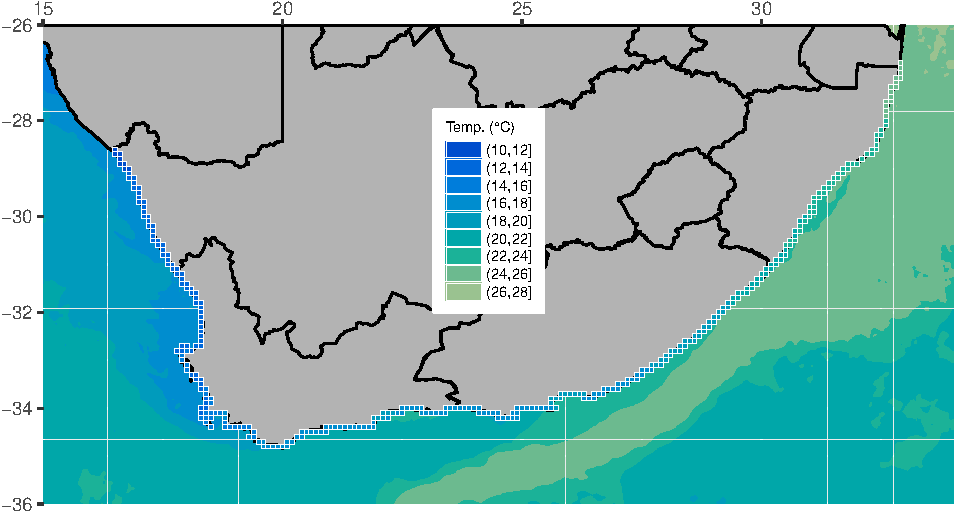
\includegraphics{08-mapping_files/figure-latex/map-final-1.pdf}
\caption{\label{fig:map-final}The cleaned up map of South Africa. Resplendent with coastal and ocean temperatures (°C).}
\end{figure}

That is a very clean looking map so let's go ahead and save it on our computers

\begin{Shaded}
\begin{Highlighting}[]
\KeywordTok{ggsave}\NormalTok{(}\DataTypeTok{plot =}\NormalTok{ final\_map, }\StringTok{"figures/map\_complete.pdf"}\NormalTok{, }\DataTypeTok{height =} \DecValTok{6}\NormalTok{, }\DataTypeTok{width =} \DecValTok{9}\NormalTok{)}
\end{Highlighting}
\end{Shaded}

\hypertarget{session-info-6}{%
\section{Session info}\label{session-info-6}}

\begin{Shaded}
\begin{Highlighting}[]
\KeywordTok{installed.packages}\NormalTok{()[}\KeywordTok{names}\NormalTok{(}\KeywordTok{sessionInfo}\NormalTok{()}\OperatorTok{$}\NormalTok{otherPkgs), }\StringTok{"Version"}\NormalTok{]}
\end{Highlighting}
\end{Shaded}

\begin{verbatim}
R>    ggpubr  magrittr   forcats   stringr     dplyr     purrr     readr     tidyr 
R>   "0.2.4"     "1.5"   "0.4.0"   "1.4.0"   "0.8.3"   "0.3.3"   "1.3.1"   "1.0.0" 
R>    tibble   ggplot2 tidyverse 
R>   "2.1.3"   "3.2.1"   "1.3.0"
\end{verbatim}

\hypertarget{mapping_style}{%
\chapter{Mapping with style}\label{mapping_style}}

\begin{quote}
``How beautiful the world was when one looked at it without searching, just looked, simply and innocently.''

--- Hermann Hesse, Siddartha
\end{quote}

\begin{quote}
``You can't judge a book by it's cover but you can sure sell a bunch of books if you have a good one.''

--- Jayce O'Neal
\end{quote}

Now that we have learned the basics of creating a beautiful map in \textbf{\texttt{ggplot2}} it is time to look at some of the more particular things we will need to make our maps extra stylish. There are also a few more things we need to learn how to do before our maps can be truly publication quality.

If we have not yet loaded the \textbf{\texttt{tidyverse}} let's do so.

\begin{Shaded}
\begin{Highlighting}[]
\CommentTok{\# Load libraries}
\KeywordTok{library}\NormalTok{(tidyverse)}
\KeywordTok{library}\NormalTok{(scales)}
\KeywordTok{library}\NormalTok{(ggsn)}

\CommentTok{\# Load Africa map}
\KeywordTok{load}\NormalTok{(}\StringTok{"data/africa\_map.RData"}\NormalTok{)}
\end{Highlighting}
\end{Shaded}

\hypertarget{default-maps}{%
\section{Default maps}\label{default-maps}}

In order to access the default maps included with the \textbf{\texttt{tidyverse}} we will use the function \texttt{borders()}.

\begin{Shaded}
\begin{Highlighting}[]
\KeywordTok{ggplot}\NormalTok{() }\OperatorTok{+}
\StringTok{  }\KeywordTok{borders}\NormalTok{() }\OperatorTok{+}\StringTok{ }\CommentTok{\# The global shape file}
\StringTok{  }\KeywordTok{coord\_equal}\NormalTok{() }\CommentTok{\# Equal sizing for lon/lat }
\end{Highlighting}
\end{Shaded}

\begin{figure}
\centering
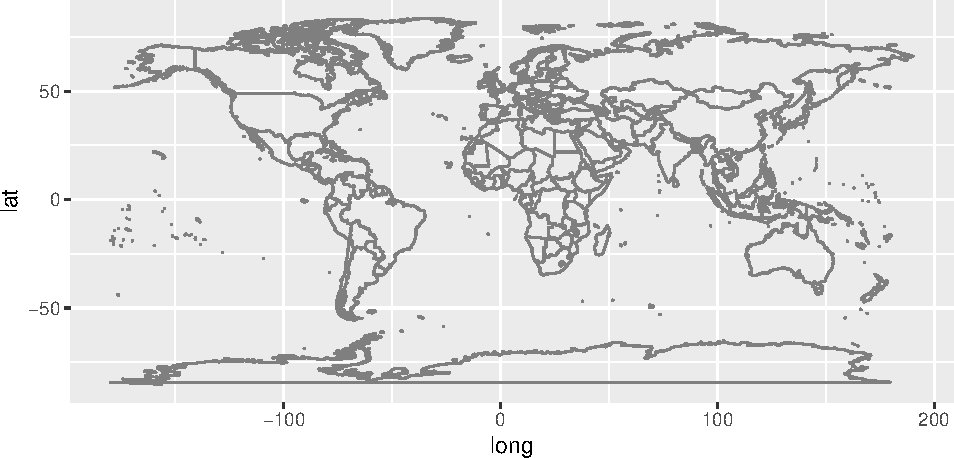
\includegraphics{09-mapping_style_files/figure-latex/maps-world-1.pdf}
\caption{\label{fig:maps-world}The built in global shape file.}
\end{figure}

Jikes! It's as simple as that to load a map of the whole planet. Usually we are not going to want to make a map of the entire planet, so let's see how to focus on just the area around South Africa.

\begin{Shaded}
\begin{Highlighting}[]
\NormalTok{sa\_}\DecValTok{1}\NormalTok{ <{-}}\StringTok{ }\KeywordTok{ggplot}\NormalTok{() }\OperatorTok{+}
\StringTok{  }\KeywordTok{borders}\NormalTok{(}\DataTypeTok{fill =} \StringTok{"grey70"}\NormalTok{, }\DataTypeTok{colour =} \StringTok{"black"}\NormalTok{) }\OperatorTok{+}
\StringTok{  }\KeywordTok{coord\_equal}\NormalTok{(}\DataTypeTok{xlim =} \KeywordTok{c}\NormalTok{(}\DecValTok{12}\NormalTok{, }\DecValTok{36}\NormalTok{), }\DataTypeTok{ylim =} \KeywordTok{c}\NormalTok{(}\OperatorTok{{-}}\DecValTok{38}\NormalTok{, }\DecValTok{{-}22}\NormalTok{), }\DataTypeTok{expand =} \DecValTok{0}\NormalTok{) }\CommentTok{\# Force lon/lat extent}
\NormalTok{sa\_}\DecValTok{1}
\end{Highlighting}
\end{Shaded}

\begin{figure}
\centering
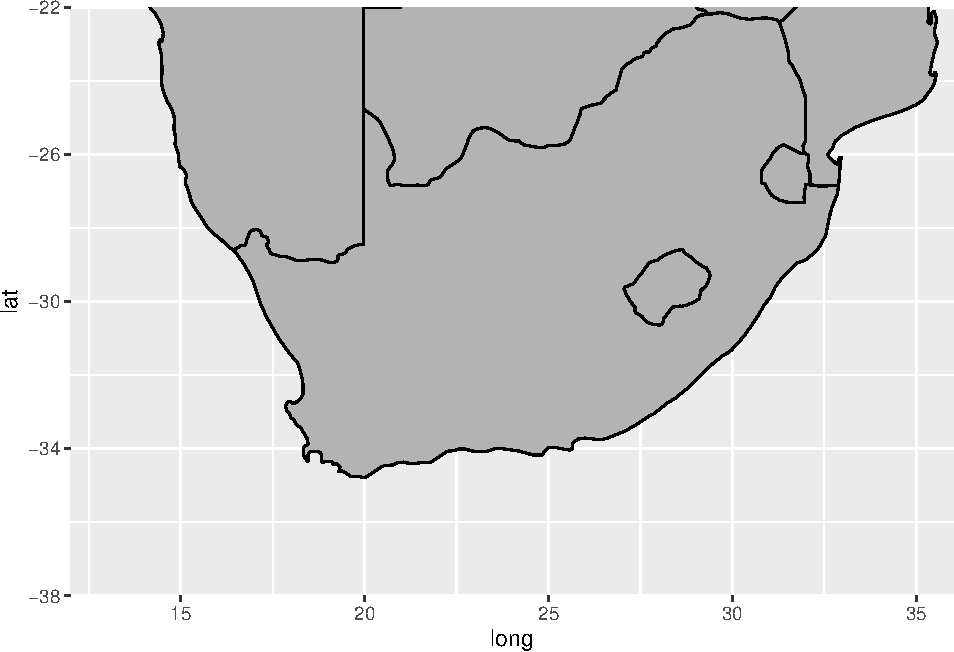
\includegraphics{09-mapping_style_files/figure-latex/maps-SA-1-1.pdf}
\caption{\label{fig:maps-SA-1}A better way to get the map of South Africa.}
\end{figure}

That is a very tidy looking map of South(ern) Africa without needing to load any files.

\hypertarget{specific-labels}{%
\section{Specific labels}\label{specific-labels}}

A map is almost always going to need some labels and other visual cues. We saw in the previous section how to add site labels. The following code chunk shows how this differs if we want to add just one label at a time. This can be useful if each label needs to be different from all other labels for whatever reason. We may also see that the text labels we are creating have \texttt{\textbackslash{}n} in them. When R sees these two characters together like this it reads this as an instruction to return down a line. Let's run the code to make sure we see what this means.

\begin{Shaded}
\begin{Highlighting}[]
\NormalTok{sa\_}\DecValTok{2}\NormalTok{ <{-}}\StringTok{ }\NormalTok{sa\_}\DecValTok{1} \OperatorTok{+}
\StringTok{  }\KeywordTok{annotate}\NormalTok{(}\StringTok{"text"}\NormalTok{, }\DataTypeTok{label =} \StringTok{"Atlantic}\CharTok{\textbackslash{}n}\StringTok{Ocean"}\NormalTok{, }
           \DataTypeTok{x =} \FloatTok{15.1}\NormalTok{, }\DataTypeTok{y =} \FloatTok{{-}32.0}\NormalTok{, }
           \DataTypeTok{size =} \FloatTok{5.0}\NormalTok{, }
           \DataTypeTok{angle =} \DecValTok{30}\NormalTok{, }
           \DataTypeTok{colour =} \StringTok{"navy"}\NormalTok{) }\OperatorTok{+}
\StringTok{  }\KeywordTok{annotate}\NormalTok{(}\StringTok{"text"}\NormalTok{, }\DataTypeTok{label =} \StringTok{"Indian}\CharTok{\textbackslash{}n}\StringTok{Ocean"}\NormalTok{, }
           \DataTypeTok{x =} \FloatTok{33.2}\NormalTok{, }\DataTypeTok{y =} \FloatTok{{-}34.2}\NormalTok{, }
           \DataTypeTok{size =} \FloatTok{5.0}\NormalTok{, }
           \DataTypeTok{angle =} \DecValTok{330}\NormalTok{, }
           \DataTypeTok{colour =} \StringTok{"springgreen"}\NormalTok{)}
\NormalTok{sa\_}\DecValTok{2}
\end{Highlighting}
\end{Shaded}

\begin{figure}
\centering
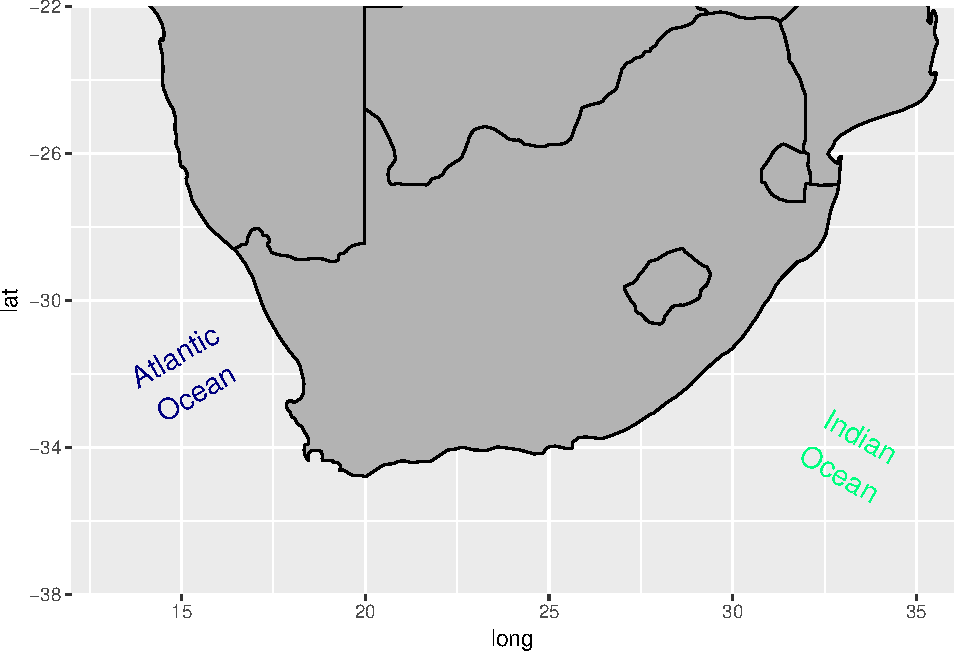
\includegraphics{09-mapping_style_files/figure-latex/maps-labels-1.pdf}
\caption{\label{fig:maps-labels}Map of southern Africa with specific labels.}
\end{figure}

\hypertarget{scale-bars}{%
\section{Scale bars}\label{scale-bars}}

With our fancy labels added, let's insert a scale bar next. There is no default scale bar function in the \textbf{\texttt{tidyverse}}, which is why we have loaded the \textbf{\texttt{ggsn}} package. This package is devoted to adding scale bars and North arrows to \textbf{\texttt{ggplot2}} figures. There are heaps of options so we'll just focus on one of them for now. It is a bit finicky so to get it looking exactly how we want it requires some guessing and checking. Please feel free to play around with the coordinates below. We may see the list of available North arrow shapes by running \texttt{northSymbols()}.

\begin{Shaded}
\begin{Highlighting}[]
\NormalTok{sa\_}\DecValTok{3}\NormalTok{ <{-}}\StringTok{ }\NormalTok{sa\_}\DecValTok{2} \OperatorTok{+}
\StringTok{  }\CommentTok{\# scalebar(x.min = 22, x.max = 26, y.min = {-}36, y.max = {-}35, \# Set location of bar}
\StringTok{  }\CommentTok{\#          dist = 200, height = 1, st.dist = 0.8, st.size = 4, \# Set particulars}
\StringTok{  }\CommentTok{\#          transform = TRUE, model = "WGS84") + \# Set appearance}
\StringTok{  }\KeywordTok{north}\NormalTok{(}\DataTypeTok{x.min =} \FloatTok{22.5}\NormalTok{, }\DataTypeTok{x.max =} \FloatTok{25.5}\NormalTok{, }\DataTypeTok{y.min =} \DecValTok{{-}33}\NormalTok{, }\DataTypeTok{y.max =} \DecValTok{{-}31}\NormalTok{, }\CommentTok{\# Set location of symbol}
        \DataTypeTok{scale =} \FloatTok{1.2}\NormalTok{, }\DataTypeTok{symbol =} \DecValTok{16}\NormalTok{)}
\NormalTok{sa\_}\DecValTok{3}
\end{Highlighting}
\end{Shaded}

\begin{figure}
\centering
\includegraphics{09-mapping_style_files/figure-latex/maps-scale-1.pdf}
\caption{\label{fig:maps-scale}Map of southern Africa with labels and a scale bar.}
\end{figure}

\hypertarget{insetting}{%
\section{Insetting}\label{insetting}}

In order to inset a smaller map inside of a larger map we must first create the smaller map. We have already loaded just such a map of Africa so we will use that for this example.

\begin{Shaded}
\begin{Highlighting}[]
\NormalTok{africa\_map}
\end{Highlighting}
\end{Shaded}

\begin{center}\includegraphics{09-mapping_style_files/figure-latex/maps-mini-1} \end{center}

And now to inset this map of Africa into our map of southern Africa we will need to learn how to create a `grob'. This is very simple and does not require any extra work on our part. Remember that \textbf{\texttt{ggplot2}} objects are different from normal objects (i.e.~dataframes), and that they have their own way of storing and accessing data. In order to convert any sort of thing into a format that ggplot understands we convert it into a grob, as shown below. Once converted, we may then plop it onto our figure/map wherever we please. Both of these steps are accomplished with the single function \texttt{annotation\_custom()}. This is also a good way to add logos or any other sort of image to a map/figure. You can really go completely bananas. It's even possible to add GIFs. Such happy. Much excite. Very wonderment.

\begin{Shaded}
\begin{Highlighting}[]
\NormalTok{sa\_}\DecValTok{4}\NormalTok{ <{-}}\StringTok{ }\NormalTok{sa\_}\DecValTok{3} \OperatorTok{+}
\StringTok{  }\KeywordTok{annotation\_custom}\NormalTok{(}\DataTypeTok{grob =} \KeywordTok{ggplotGrob}\NormalTok{(africa\_map),}
                    \DataTypeTok{xmin =} \FloatTok{20.9}\NormalTok{, }\DataTypeTok{xmax =} \FloatTok{26.9}\NormalTok{,}
                    \DataTypeTok{ymin =} \DecValTok{{-}30}\NormalTok{, }\DataTypeTok{ymax =} \DecValTok{{-}24}\NormalTok{)}
\NormalTok{sa\_}\DecValTok{4}
\end{Highlighting}
\end{Shaded}

\begin{figure}
\centering
\includegraphics{09-mapping_style_files/figure-latex/maps-inset-1.pdf}
\caption{\label{fig:maps-inset}Map of southern Africa, with labels, scale bar, and an inset map of Africa.}
\end{figure}

\hypertarget{rounding-it-out}{%
\section{Rounding it out}\label{rounding-it-out}}

There are a lot of exciting things going on in our figure now. To round out our adventures in mapping let's tweak the lon/lat labels to a more prestigious convention. There are two ways to do this. One of which requires us to install the \textbf{\texttt{scales}} package. Don't worry, it's a small one!

\begin{Shaded}
\begin{Highlighting}[]
\NormalTok{sa\_final <{-}}\StringTok{ }\NormalTok{sa\_}\DecValTok{4} \OperatorTok{+}
\StringTok{  }\KeywordTok{scale\_x\_continuous}\NormalTok{(}\DataTypeTok{breaks =} \KeywordTok{seq}\NormalTok{(}\DecValTok{16}\NormalTok{, }\DecValTok{32}\NormalTok{, }\DecValTok{4}\NormalTok{),}
                     \DataTypeTok{labels =} \KeywordTok{c}\NormalTok{(}\StringTok{"16°E"}\NormalTok{, }\StringTok{"20°E"}\NormalTok{, }\StringTok{"24°E"}\NormalTok{, }\StringTok{"28°E"}\NormalTok{, }\StringTok{"32°E"}\NormalTok{),}
                     \DataTypeTok{position =} \StringTok{"bottom"}\NormalTok{) }\OperatorTok{+}
\StringTok{  }\KeywordTok{scale\_y\_continuous}\NormalTok{(}\DataTypeTok{breaks =} \KeywordTok{seq}\NormalTok{(}\OperatorTok{{-}}\DecValTok{36}\NormalTok{, }\DecValTok{{-}24}\NormalTok{, }\DecValTok{4}\NormalTok{),}
                     \DataTypeTok{labels =} \KeywordTok{c}\NormalTok{(}\StringTok{"36.0°S"}\NormalTok{, }\StringTok{"32.0°S"}\NormalTok{, }\StringTok{"28.0°S"}\NormalTok{, }\StringTok{"24.0°S"}\NormalTok{),}
                     \DataTypeTok{position =} \StringTok{"right"}\NormalTok{) }\OperatorTok{+}
\StringTok{  }\KeywordTok{labs}\NormalTok{(}\DataTypeTok{x =} \StringTok{""}\NormalTok{, }\DataTypeTok{y =} \StringTok{""}\NormalTok{)}
\NormalTok{sa\_final}
\end{Highlighting}
\end{Shaded}

\begin{figure}
\centering
\includegraphics{09-mapping_style_files/figure-latex/maps-final-1.pdf}
\caption{\label{fig:maps-final}The final map with all of the bells and whistles.}
\end{figure}

And lastly we save the fruits of our labours.

\begin{Shaded}
\begin{Highlighting}[]
\KeywordTok{ggsave}\NormalTok{(}\DataTypeTok{plot =}\NormalTok{ sa\_final, }\DataTypeTok{filename =} \StringTok{"figures/southern\_africa\_final.pdf"}\NormalTok{, }
       \DataTypeTok{height =} \DecValTok{6}\NormalTok{, }\DataTypeTok{width =} \DecValTok{8}\NormalTok{)}
\end{Highlighting}
\end{Shaded}

\hypertarget{session-info-7}{%
\section{Session info}\label{session-info-7}}

\begin{Shaded}
\begin{Highlighting}[]
\KeywordTok{installed.packages}\NormalTok{()[}\KeywordTok{names}\NormalTok{(}\KeywordTok{sessionInfo}\NormalTok{()}\OperatorTok{$}\NormalTok{otherPkgs), }\StringTok{"Version"}\NormalTok{]}
\end{Highlighting}
\end{Shaded}

\begin{verbatim}
R>      ggsn    scales   forcats   stringr     dplyr     purrr     readr     tidyr 
R>   "0.5.0"   "1.1.0"   "0.4.0"   "1.4.0"   "0.8.3"   "0.3.3"   "1.3.1"   "1.0.0" 
R>    tibble   ggplot2 tidyverse 
R>   "2.1.3"   "3.2.1"   "1.3.0"
\end{verbatim}

\hypertarget{mapping_google}{%
\chapter{Mapping with Google}\label{mapping_google}}

\begin{quote}
``The only thing Google has failed to do, so far, is fail.''

--- John Battelle
\end{quote}

\begin{quote}
``I'm afraid that if you look at a thing long enough, it loses all of its meaning.''

--- Andy Warhol
\end{quote}

Now that we've seen how to produce complex maps with \textbf{\texttt{ggplot2}} we are going to learn how to bring Google maps into the mix. Some kind hearted person has made a package for R that allows us to do this relatively easily. But that means we will need to install another new package.

After we learn how to use Google maps we will take some time to learn additional mapping techniques that we may want for creating publication quality figures.

\hypertarget{ggmap}{%
\section{\texorpdfstring{\textbf{\texttt{ggmap}}}{ggmap}}\label{ggmap}}

The package we will need for this tut is \textbf{\texttt{ggmap}}. It is a bit beefy so let's get started on installing it now. Once it's done we will activated the packages we need and load some site points for mapping.

\begin{Shaded}
\begin{Highlighting}[]
\CommentTok{\# Load libraries}
\KeywordTok{library}\NormalTok{(tidyverse)}
\KeywordTok{library}\NormalTok{(ggmap)}

\CommentTok{\# Load data}
\KeywordTok{load}\NormalTok{(}\StringTok{"data/cape\_point\_sites.RData"}\NormalTok{)}
\end{Highlighting}
\end{Shaded}

Take a moment to look at the data we loaded. What does it show?

\hypertarget{mapping-cape-point}{%
\section{Mapping Cape Point}\label{mapping-cape-point}}

We will be creating our Google map in two steps. The first step is to use the \texttt{get\_map()} function to tell Google what area of the world we want a map of, as well as what sort of map we want. Remember how Google maps can be switched from satellite view to map view? We may do that in R as well. For now we are only going to use the satellite view so that we may insert out own labels. But if we look in the help file we may see a description of all the different map types available. There are a bunch!

The \texttt{get\_map()} function relies on a healthy Internet connection to run. The downloading of Google maps can be a tenuous process without a stable connection. For that reason, if your Internet connection is not great you may run the commented out line of code in favour of loading the Google map. This is a pre-saved file of the output of the code chunk below. Please rather run the \texttt{get\_map()} function first, and if it won't connect only then load the saved file as shown below.

\begin{Shaded}
\begin{Highlighting}[]
\NormalTok{cape\_point <{-}}\StringTok{ }\KeywordTok{get\_map}\NormalTok{(}\DataTypeTok{location =} \KeywordTok{c}\NormalTok{(}\DataTypeTok{lon =} \FloatTok{18.36519}\NormalTok{, }\DataTypeTok{lat =} \FloatTok{{-}34.2352581}\NormalTok{),}
                        \DataTypeTok{zoom =} \DecValTok{10}\NormalTok{, }\DataTypeTok{maptype =} \StringTok{\textquotesingle{}satellite\textquotesingle{}}\NormalTok{)}
\CommentTok{\# load("data/cape\_point.RData")}
\end{Highlighting}
\end{Shaded}

If we look in the environment panel in the top right corner, what do we see? What do we think the code above is doing?

The second step in the process is to treat the Google data we downloaded as though it is just any ordinary \textbf{\texttt{ggplot2}} object. The same as the ones we created yesterday and today. For this reason we may use \texttt{+} to add new lines of \textbf{\texttt{ggplot2}} code to the Google object we downloaded in order to show site locations etc. Let's first just see how the map looks when we add some points. Note that we do not use the function \texttt{ggplot()} at the beginning of our code, but rather \texttt{ggmap()}.

\begin{Shaded}
\begin{Highlighting}[]
\NormalTok{cp\_}\DecValTok{1}\NormalTok{ <{-}}\StringTok{ }\KeywordTok{ggmap}\NormalTok{(cape\_point) }\OperatorTok{+}
\StringTok{  }\KeywordTok{geom\_point}\NormalTok{(}\DataTypeTok{data =}\NormalTok{ cape\_point\_sites, }\KeywordTok{aes}\NormalTok{(}\DataTypeTok{x =}\NormalTok{ lon}\FloatTok{+0.002}\NormalTok{, }\DataTypeTok{y =}\NormalTok{ lat}\FloatTok{{-}0.007}\NormalTok{), }
             \DataTypeTok{colour =} \StringTok{"red"}\NormalTok{, }\DataTypeTok{size =}  \FloatTok{2.5}\NormalTok{) }\OperatorTok{+}
\StringTok{  }\KeywordTok{labs}\NormalTok{(}\DataTypeTok{x =} \StringTok{""}\NormalTok{, }\DataTypeTok{y =} \StringTok{""}\NormalTok{)}
\NormalTok{cp\_}\DecValTok{1}
\end{Highlighting}
\end{Shaded}

\begin{figure}
\centering
\includegraphics{10-mapping_google_files/figure-latex/ggmap-1-1.pdf}
\caption{\label{fig:ggmap-1}Google map of Cape Point with some site locations highlighted with red points.}
\end{figure}

Pretty cool huh?! You may do this for anywhere in the world just as easy as this. The only thing you need to keep in mind is that the lon/lat coordinates for Google appear to be slightly different than the global standard. This is why the x and y \texttt{aes()} values in the code above have a little bit added or subtracted from them. That one small issue aside, this is a nice quick workflow for adding your site locations to a Google map background. Play around with the different map types you can download and try it for any place you can think of.

\hypertarget{site-labels}{%
\section{Site labels}\label{site-labels}}

The previous figure shows our sites along Cape Point, which is great, but which site is which?! We need site labels. This is a relatively straightforward process, so we've given a complicated example of how to do so here.

\begin{Shaded}
\begin{Highlighting}[]
\NormalTok{cp\_}\DecValTok{2}\NormalTok{ <{-}}\StringTok{ }\NormalTok{cp\_}\DecValTok{1} \OperatorTok{+}
\StringTok{  }\KeywordTok{geom\_text}\NormalTok{(}\DataTypeTok{data =}\NormalTok{ cape\_point\_sites, }\CommentTok{\# Choose dataframe}
            \KeywordTok{aes}\NormalTok{(lon}\FloatTok{+0.002}\NormalTok{, lat}\FloatTok{{-}0.007}\NormalTok{, }\DataTypeTok{label =}\NormalTok{ site), }\CommentTok{\# Set aesthetics}
            \DataTypeTok{hjust =} \FloatTok{1.15}\NormalTok{, }\DataTypeTok{vjust =} \FloatTok{0.5}\NormalTok{, }\CommentTok{\# Adjust vertical and horizontal}
            \DataTypeTok{size =} \DecValTok{3}\NormalTok{, }\DataTypeTok{colour =} \StringTok{"white"}\NormalTok{) }\CommentTok{\# Adjust appearance}
\NormalTok{cp\_}\DecValTok{2}
\end{Highlighting}
\end{Shaded}

\begin{figure}
\centering
\includegraphics{10-mapping_google_files/figure-latex/ggmap-2-1.pdf}
\caption{\label{fig:ggmap-2}Google map of Cape Point with site point labeled}
\end{figure}

\hypertarget{diy-maps}{%
\section{DIY maps}\label{diy-maps}}

Now that we have learned how to make conventional maps, as well as fancy Google maps, it is time for us to branch out once again at let our creative juices flow. Please group up as you see fit and create your own beautiful map of wherever you like. Bonus points for faceting in additional figures showing supplementary information. Feel free to use either conventional maps or the Google alternative. Same as yesterday, we will be walking the room to help with any issues that may arise.

\hypertarget{session-info-8}{%
\section{Session info}\label{session-info-8}}

\begin{Shaded}
\begin{Highlighting}[]
\KeywordTok{installed.packages}\NormalTok{()[}\KeywordTok{names}\NormalTok{(}\KeywordTok{sessionInfo}\NormalTok{()}\OperatorTok{$}\NormalTok{otherPkgs), }\StringTok{"Version"}\NormalTok{]}
\end{Highlighting}
\end{Shaded}

\begin{verbatim}
R>     ggmap   forcats   stringr     dplyr     purrr     readr     tidyr    tibble 
R>   "3.0.0"   "0.4.0"   "1.4.0"   "0.8.3"   "0.3.3"   "1.3.1"   "1.0.0"   "2.1.3" 
R>   ggplot2 tidyverse 
R>   "3.2.1"   "1.3.0"
\end{verbatim}

\hypertarget{tidy}{%
\chapter{Tidy data}\label{tidy}}

\begin{quote}
``Order and simplification are the first steps toward the mastery of a subject.''

--- Thomas Mann
\end{quote}

\begin{quote}
``Get your facts first, and then you can distort them as much as you please.''

--- Mark Twain
\end{quote}

The \href{http://tidyverse.org}{Tidyverse} is a collection of R packages that adhere to the \emph{tidy data} principles of data analysis and graphing. The purpose of these packages is to make working with data more efficient. The core Tidyverse packages were created by Hadley Wickham, but over the last few years other individuals have added some packages to the collective, which has significantly expanded our data analytical capabilities through improved ease of use and efficiency. The Tidyverse packages can be loaded collectively by calling the \textbf{\texttt{tidyverse}} package, as we have seen throughout this workshop. The packages making up the Tidyverse are shown in Figure \ref{fig:tidyverse}.

\begin{figure}

{\centering \includegraphics[width=1\linewidth]{figures/tidyverse} 

}

\caption{The Tidyverse by Hadley Wickham and co.}\label{fig:tidyverse}
\end{figure}

\begin{Shaded}
\begin{Highlighting}[]
\KeywordTok{library}\NormalTok{(tidyverse)}
\end{Highlighting}
\end{Shaded}

As we may see in the following figure (Figure \ref{fig:tidy}), the tidying of ones data should be the second step in any workflow, after the loading of the data.

\begin{figure}

{\centering \includegraphics[width=1\linewidth]{figures/data-science-wrangle} 

}

\caption{Data tidying in the data processing pipeline. Reproduced from [R for Data Science](http://r4ds.had.co.nz/workflow-basics.html)}\label{fig:tidy}
\end{figure}

But what exactly are \textbf{tidy data}? It is not just a a buzz word, there is a real definition. In three parts, to be exact. Taken from Hadley Wickham's \href{http://r4ds.had.co.nz/workflow-basics.html}{R for Data Science}:

\begin{quote}
\begin{enumerate}
\def\labelenumi{\arabic{enumi}.}
\tightlist
\item
  Each variable must have its own column---i.e.~each of the things known \emph{about} the data in its own column.
\item
  Each observation must have its own row---each of the things \emph{measured} in its own row; for example, in the \emph{Laminaria} data the measured things include \texttt{blade\_length}, \texttt{blade\_weight}, etc., and they can all be captured in one column named, for example, \texttt{measurement}.\\
\item
  Each value must have its own cell---each of the things that are known or measured must be in its own cell.
\end{enumerate}
\end{quote}

This is represented graphically in figure \ref{fig:tidy-structure}. One will generally satisfy these three rules effortlessly simply by never putting more than one dataset in a file, and never putting more (or less) than one variable in the same column. We will go over this several more times today so do not fret if those guidelines are not immediately clear.

\begin{figure}

{\centering \includegraphics[width=1\linewidth]{figures/tidy-1} 

}

\caption{Following three rules make a dataset tidy --- variables are in columns, observations are in rows, and values are in cells. Reproduced from [R for Data Science](http://r4ds.had.co.nz/workflow-basics.html)}\label{fig:tidy-structure}
\end{figure}

In order to illustrate the meaning of this three part definition we are going to learn how to manipulate a non-tidy dataset into a tidy one. To do so we will need to learn a few new, very useful functions. Let's load our demo dataset to get started. This snippet from the SACTN dataset contains only data for 2008-2009 for three time series, with some notable (untidy) changes. The purpose of the following exercises is not only to show how to tidy data, but to also illustrate that these steps may be done more quickly in R than excel, allowing for ones raw data to remain exactly how they were collected, with all of the manipulations performed on them documented in an R script. This is a centrally important part of reproducible research.

\begin{Shaded}
\begin{Highlighting}[]
\KeywordTok{load}\NormalTok{(}\StringTok{"data/SACTN\_mangled.RData"}\NormalTok{)}
\end{Highlighting}
\end{Shaded}

With our data loaded let's now have a peek at them. We will first see that we have loaded not one, but five different objects into our environment pane in the top left our RStudio window. These all contain the exact same data in different states of disrepair. As one may guess, some of these datasets will be easier to use than others.

\begin{Shaded}
\begin{Highlighting}[]
\NormalTok{SACTN1}
\NormalTok{SACTN2}
\NormalTok{SACTN3}

\CommentTok{\# Spread across two dataframes}
\NormalTok{SACTN4a}
\NormalTok{SACTN4b}
\end{Highlighting}
\end{Shaded}

We start off by looking at \texttt{SACTN1}. If these data look just like all of the other SACTN data we've used thus far that's because they are. These are how tidy data should look. No surprises. In fact, because these data are already tidy it is very straightforward to use them for whatever purposes we may want. Making a time series plot, for example.

\begin{Shaded}
\begin{Highlighting}[]
\KeywordTok{ggplot}\NormalTok{(}\DataTypeTok{data =}\NormalTok{ SACTN1, }\KeywordTok{aes}\NormalTok{(}\DataTypeTok{x =}\NormalTok{ date, }\DataTypeTok{y =}\NormalTok{ temp)) }\OperatorTok{+}
\StringTok{  }\KeywordTok{geom\_line}\NormalTok{(}\KeywordTok{aes}\NormalTok{(}\DataTypeTok{colour =}\NormalTok{ site, }\DataTypeTok{group =} \KeywordTok{paste0}\NormalTok{(site, src))) }\OperatorTok{+}
\StringTok{  }\KeywordTok{labs}\NormalTok{(}\DataTypeTok{x =} \StringTok{""}\NormalTok{, }\DataTypeTok{y =} \StringTok{"Temperature (°C)"}\NormalTok{, }\DataTypeTok{colour =} \StringTok{"Site"}\NormalTok{) }\OperatorTok{+}
\StringTok{  }\KeywordTok{theme\_bw}\NormalTok{()}
\end{Highlighting}
\end{Shaded}

\includegraphics{11-tidy_files/figure-latex/tidy-1-1.pdf}

\begin{quote}
\textbf{\texttt{\%\textgreater{}\%}}~\\
Remember that this funny series of symbols is the pipe operator. It combines consequetive rows of code together so that they run as though they were one `chunk'. We will be seeing this symbol a lot today. The keyboard shortcut for \texttt{\%\textgreater{}\%} is \textbf{ctrl shift m}.
\end{quote}

\hypertarget{gathering-and-spreading}{%
\section{Gathering and spreading}\label{gathering-and-spreading}}

Before \emph{tidy} became the adjective used to describe neatly formatted data, people used to say \emph{long}. This is because well organised dataframes tend to always be longer than they are wide (with the exception of species assemblage data). The opposite of \emph{long} data are \emph{wide} data. If one ever finds a dataset that is wider than it is long then this is probably because the person that created them saved one variable across many columns.

As we sit here and read through these examples it may seem odd that so much effort is being spent on something so straightforward as tidy data. Surely this is too obvious to devote an entire day of work to it? Unfortunately not. As we go out into the wild world of `real life data', we tend to find that very few datasets (especially those collected by hand) are tidy. Rather they are plagued by any number of issues. The first step then for tidying up the data are to have a look at them and discern what are the observations that were made/recorded (the `measurements'), and what are the variables within those observations. We also need to know something about \emph{how} or \emph{where} the data were collected, or what threy represent --- this is information \emph{about} the data, i.e.~some meta-data. Let's have a look now at \texttt{SACTN2} for an example of what \emph{wide} data looks like, and how to fix it.

\hypertarget{gathering}{%
\subsection{Gathering}\label{gathering}}

In \texttt{SACTN2} we can see that the \texttt{src} column has been removed and that the temperatures are placed in columns that denote the collecting source. This may at first seem like a reasonable way to organise these data, but it is not tidy because the collecting source is one variable, and so should not take up more than one column. We need to \texttt{gather()} these source columns back together. We do this by telling \texttt{gather()} what the names of the columns are we want to squish together. We then tell it the name of the `key' column. This is the column that will contain all of the old column names we are gathering. In this case we will call it `src'. The last piece of this puzzle is the `value' column. This is where we decide what the name of the column will be for values we are gathering up. In this case we will name it `temp', because we are gathering up the temperature values that were incorrectly spread out by month.

\begin{Shaded}
\begin{Highlighting}[]
\NormalTok{SACTN2\_tidy <{-}}\StringTok{ }\NormalTok{SACTN2 }\OperatorTok{\%>\%}
\StringTok{  }\KeywordTok{gather}\NormalTok{(DEA, KZNSB, SAWS, }\DataTypeTok{key =} \StringTok{"src"}\NormalTok{, }\DataTypeTok{value =} \StringTok{"temp"}\NormalTok{)}
\end{Highlighting}
\end{Shaded}

\hypertarget{spreading}{%
\subsection{Spreading}\label{spreading}}

Should ones data be too long, meaning when individual observations are spread across multiple rows, we will need to use \texttt{spread()} to rectify the situation. This is generally the case when we have two or more variables stored within the same column, as we may see in \texttt{SACTN3}. This is not terribly common as it would require someone to put quite a bit of time into making a dataframe this way. But never say never. To spread data we first tell R what the name of the column is that contains more than one variable, in this case the `var' column. We then tell R what the name of the column is that contains the values that need to be spread, in this case the `val' column. Notice here that these two column names are not given in inverted commas. This is because with gather, we were creating two new columns, and so we fed them to R as character vectors (i.e.~inside of inverted commas). With the spread function we are naming existing columns and so we give them to R without inverted commas.

\begin{Shaded}
\begin{Highlighting}[]
\NormalTok{SACTN3\_tidy <{-}}\StringTok{ }\NormalTok{SACTN3 }\OperatorTok{\%>\%}\StringTok{ }
\StringTok{  }\KeywordTok{spread}\NormalTok{(}\DataTypeTok{key =}\NormalTok{ var, }\DataTypeTok{value =}\NormalTok{ val)}
\end{Highlighting}
\end{Shaded}

\hypertarget{separating-and-uniting}{%
\section{Separating and uniting}\label{separating-and-uniting}}

We've now covered how to make our dataframes longer or wider depending on their tidiness. Now we will look at how to manage our columns when they contain more (or less) than one variable, but the overall dataframe does not need to be made wider or longer. This is generally the case when one has a column with two variables, or two or more variables are spread out across multiple columns, but there is still only one observation per row. Let's see some examples to make this more clear.

\hypertarget{separate}{%
\subsection{Separate}\label{separate}}

If we look at \texttt{SACTN4a} we see that we no longer have a \texttt{site} and \texttt{src} column. Rather these have been replaced by an \texttt{index} column. This is an efficient way to store these data, but it is not tidy because the site and source of each observation have now been combined into one column (variable). Remember, tidy data calls for each of the things known about the data to be its own variable. To re-create our \texttt{site} and \texttt{src} columns we must \texttt{separate()} the \texttt{index} column. First we give R the name of the column we want to separate, in this case \texttt{index}. Next we must say what the names of the new columns will be. Remember that because we are creating new column names we feed these into R within inverted commas. Lastly we should tell R how to separate the \texttt{index} column. If we look at the data we may see that the values we want to split up are separated with `/', so that is what we give to R. Often times the \texttt{separate()} function is able to guess correctly, but it is better to be explicit.

\begin{Shaded}
\begin{Highlighting}[]
\NormalTok{SACTN4a\_tidy <{-}}\StringTok{ }\NormalTok{SACTN4a }\OperatorTok{\%>\%}\StringTok{ }
\StringTok{  }\KeywordTok{separate}\NormalTok{(}\DataTypeTok{col =}\NormalTok{ index, }\DataTypeTok{into =} \KeywordTok{c}\NormalTok{(}\StringTok{"site"}\NormalTok{, }\StringTok{"src"}\NormalTok{), }\DataTypeTok{sep =} \StringTok{"/ "}\NormalTok{)}
\end{Highlighting}
\end{Shaded}

\hypertarget{unite}{%
\subsection{Unite}\label{unite}}

It is not uncommon that field/lab instruments split values across multiple columns while they are making recordings. I see this most often with date values. Often the year, month, and day values are given in different columns. There are uses for the data in this way, though it is not terribly tidy. We usually want the date of any observation to be shown in just one column. If we look at \texttt{SACTN4b} we will see that there is a \texttt{year}, \texttt{month}, and \texttt{day} column. To \texttt{unite()} them we must first tell R what we want the united column to be labelled, in this case we will use `date'. We then list the columns to be united, her this is \texttt{year}, \texttt{month}, and \texttt{day}. Lastly we must specify if we want the united values to have a separator between them. The standard separator for date values is `-'.

\begin{Shaded}
\begin{Highlighting}[]
\NormalTok{SACTN4b\_tidy <{-}}\StringTok{ }\NormalTok{SACTN4b }\OperatorTok{\%>\%}\StringTok{ }
\StringTok{  }\KeywordTok{unite}\NormalTok{(year, month, day, }\DataTypeTok{col =} \StringTok{"date"}\NormalTok{, }\DataTypeTok{sep =} \StringTok{"{-}"}\NormalTok{)}
\end{Highlighting}
\end{Shaded}

\hypertarget{joining}{%
\section{Joining}\label{joining}}

We will end this session with the concept of joining two different dataframes. Remember that one of the rules of tidy data is that only one complete dataset is saved per dataframe. This rule then is violated not only when additional data are stored where they don't belong, but also when necessary data are saved elsewhere. If we look back at \texttt{SACTN4a} and \texttt{SACTN4b} we will see that they are each missing different columns. Were we to \textbf{join} these dataframes together they would complete each other. The \texttt{tidyverse} provides us with several methods of doing this, but we will demonstrate here only the most common technique. The function \texttt{left\_join()} is so named because it joins two or more dataframes together based on the matching of columns from the left to the right. It combines values together where it sees that they match up, and adds new rows and columns where they do not.

\begin{Shaded}
\begin{Highlighting}[]
\NormalTok{SACTN4\_tidy <{-}}\StringTok{ }\KeywordTok{left\_join}\NormalTok{(SACTN4a\_tidy, SACTN4b\_tidy)}
\end{Highlighting}
\end{Shaded}

\begin{verbatim}
R> Joining, by = c("site", "src", "date")
\end{verbatim}

As we see above, if we let \texttt{left\_join()} do it's thing it will make a plan for us and find the common columns and match up the values and observations for us best it thinks. It then returns a message letting us know what it's done. That is a pleasant convenience, but we most likely want to exert more control over this process than that. In order to specify the columns to be used for joining we must add one more argument to \texttt{left\_join()}. The \texttt{by} argument must be fed a list of column names in inverted commas if we want to specify how to join our dataframes. Not that when we run this it does not produce a message as we have provided enough explicit information that the machine is no longer needing to think for itself.

\begin{Shaded}
\begin{Highlighting}[]
\NormalTok{SACTN4\_tidy <{-}}\StringTok{ }\KeywordTok{left\_join}\NormalTok{(SACTN4a\_tidy, SACTN4b\_tidy, }\DataTypeTok{by =} \KeywordTok{c}\NormalTok{(}\StringTok{"site"}\NormalTok{, }\StringTok{"src"}\NormalTok{, }\StringTok{"date"}\NormalTok{))}
\end{Highlighting}
\end{Shaded}

\hypertarget{but-why-though}{%
\section{But why though?}\label{but-why-though}}

At this point one may be wondering what the point of all of this is. Sure it's all well and good to see how to tidy one's data in R, but couldn't this be done more quickly and easily in Excel? Perhaps, yes, with a small dataset. But remember, (for many) the main reason we are learning R is to ensure that we are performing reproducible research. This means that every step in our workflow must be documented. And we accomplish this by writing R scripts.

\hypertarget{exercise-4}{%
\chapter{Exercise}\label{exercise-4}}

Create two vectors: x \textless- c( 1, 6, 21, 19 , NA, 73, NA) and y \textless- c(NA, NA, 3, NA, 13, 24, NA)

\begin{enumerate}
\def\labelenumi{\alph{enumi})}
\item
  Count the number of elements are missing in both x and y
\item
  Transform the code, used above (a), into a function
\item
  Create three new vectors and test the function created in (b)
\end{enumerate}

\hypertarget{session-info-9}{%
\section{Session info}\label{session-info-9}}

\begin{Shaded}
\begin{Highlighting}[]
\KeywordTok{installed.packages}\NormalTok{()[}\KeywordTok{names}\NormalTok{(}\KeywordTok{sessionInfo}\NormalTok{()}\OperatorTok{$}\NormalTok{otherPkgs), }\StringTok{"Version"}\NormalTok{]}
\end{Highlighting}
\end{Shaded}

\begin{verbatim}
R>   forcats   stringr     dplyr     purrr     readr     tidyr    tibble   ggplot2 
R>   "0.4.0"   "1.4.0"   "0.8.3"   "0.3.3"   "1.3.1"   "1.0.0"   "2.1.3"   "3.2.1" 
R> tidyverse 
R>   "1.3.0"
\end{verbatim}

\hypertarget{tidier}{%
\chapter{Tidier data}\label{tidier}}

\begin{quote}
``Knowing where things are, and why, is essential to rational decision making.''

--- Jack Dangermond
\end{quote}

\begin{quote}
``The mind commands the body and it obeys. The mind orders itself and meets resistance.''

--- Frank Herbert, Dune
\end{quote}

On Day 1 already we walked ourselves through a tidy workflow. We saw how to import data, how to manipulate it, run a quick analysis or two, and create figures. In the previous session we filled in the missing piece of the workflow by also learning how to tidy up our data within R. For the remainder of today we will be revisiting the `transform' portion of the tidy workflow. In this session we are going to go into more depth on what we learned in Day 1, and in the last session we will learn some new tricks. Over these two sessions we will also become more comfortable with the \emph{pipe} command \texttt{\%\textgreater{}\%}, while practising writing tidy code.

There are five primary data transformation functions that we will focus on here:

\begin{itemize}
\tightlist
\item
  Arrange observations (rows) with \texttt{arrange()}\\
\item
  Filter observations (rows) with \texttt{filter()}\\
\item
  Select variables (columns) with\texttt{select()}\\
\item
  Create new variables (columns) with \texttt{mutate()}\\
\item
  Summarise variables (columns) with \texttt{summarise()}
\end{itemize}

We will use the full South African Coastal Temperature Network dataset for these exercises. Before we begin however we will need to cover two new concepts.

\begin{Shaded}
\begin{Highlighting}[]
\CommentTok{\# Load libraries}
\KeywordTok{library}\NormalTok{(tidyverse)}
\KeywordTok{library}\NormalTok{(lubridate)}

\CommentTok{\# Load the data from a .RData file}
\KeywordTok{load}\NormalTok{(}\StringTok{"data/SACTNmonthly\_v4.0.RData"}\NormalTok{)}

\CommentTok{\# Copy the data as a dataframe with a shorter name}
\NormalTok{SACTN <{-}}\StringTok{ }\NormalTok{SACTNmonthly\_v4}\FloatTok{.0}

\CommentTok{\# Remove the original}
\KeywordTok{rm}\NormalTok{(SACTNmonthly\_v4}\FloatTok{.0}\NormalTok{)}
\end{Highlighting}
\end{Shaded}

\hypertarget{comparison-operators}{%
\section{Comparison operators}\label{comparison-operators}}

The assignment operator (\texttt{\textless{}-}) is a symbol that we use to assign some bit of code to an object in our environment. Likewise, comparison operators are symbols we use to compare different objects. This is how we tell R how to decide to do many different things. We will see these symbols often out in the `real world' so let's spend a moment now getting to know them better. Most of these should be very familiar to us:

\begin{itemize}
\tightlist
\item
  Greater than: \texttt{\textgreater{}}\\
\item
  Greater than or equal to: \texttt{\textgreater{}=}\\
\item
  Less than: \texttt{\textless{}}\\
\item
  Less than or equal to: \texttt{\textless{}=}\\
\item
  Equal to: \texttt{==}\\
\item
  Not equal to: \texttt{!=}
\end{itemize}

It is important here to note that \texttt{==} is for comparisons and \texttt{=} is for maths. They are \textbf{not} interchangeable, as we may see in the following code chunk. This is one of the more common mistakes one makes when writing code. Luckily the error message this creates should provide us with the clues we need to figure out that we have made this specific mistake.

\begin{Shaded}
\begin{Highlighting}[]
\NormalTok{SACTN }\OperatorTok{\%>\%}\StringTok{ }
\StringTok{  }\KeywordTok{filter}\NormalTok{(}\DataTypeTok{site =} \StringTok{"Amanzimtoti"}\NormalTok{)}
\end{Highlighting}
\end{Shaded}

\begin{verbatim}
R> Error: `site` (`site = "Amanzimtoti"`) must not be named, do you need `==`?
\end{verbatim}

\hypertarget{logical-operators}{%
\section{Logical operators}\label{logical-operators}}

Comparison operators are used to make direct comparisons between specific things, but logical operators are used more broadly when making logical arguments. Logic is central to most computing so it is worth taking the time to cover these symbols explicitly here. R makes use of the same \emph{Boolean logic} symbols as many other platforms, including Google, so some (or all) of these will likely be familiar. We will generally only use three:

\begin{itemize}
\tightlist
\item
  and: \texttt{\&}\\
\item
  or: \texttt{\textbar{}}\\
\item
  not: \texttt{!}
\end{itemize}

When writing a line of tidy code we tend to use these logical operator to combine two or more arguments that use comparison operators. For example, the following code chunk uses the \texttt{filter()} function to find all temperatures recorded at Pollock Beach during December \textbf{OR} January. Don't worry if the following line of code is difficult to piece out, but make sure you can locate which symbols are comparison operators and which are logical operators. Please note that for purposes of brevity all of the outputs in this section are limited to ten lines, but when one runs these code chunks on ones own computer they will be much longer.

\begin{Shaded}
\begin{Highlighting}[]
\NormalTok{SACTN }\OperatorTok{\%>\%}\StringTok{ }
\StringTok{  }\KeywordTok{filter}\NormalTok{(site }\OperatorTok{==}\StringTok{ "Pollock Beach"}\NormalTok{, }\KeywordTok{month}\NormalTok{(date) }\OperatorTok{==}\StringTok{ }\DecValTok{12} \OperatorTok{|}\StringTok{ }\KeywordTok{month}\NormalTok{(date) }\OperatorTok{==}\StringTok{ }\DecValTok{1}\NormalTok{)}
\end{Highlighting}
\end{Shaded}

\begin{verbatim}
R>             site  src       date     temp depth   type
R> 1  Pollock Beach SAWS 1999-12-01 19.95000     0 thermo
R> 2  Pollock Beach SAWS 2000-01-01 19.03333     0 thermo
R> 3  Pollock Beach SAWS 2000-12-01 19.20000     0 thermo
R> 4  Pollock Beach SAWS 2001-01-01 18.32667     0 thermo
R> 5  Pollock Beach SAWS 2001-12-01 20.59032     0 thermo
R> 6  Pollock Beach SAWS 2002-01-01 21.47097     0 thermo
R> 7  Pollock Beach SAWS 2002-12-01 19.78065     0 thermo
R> 8  Pollock Beach SAWS 2003-01-01 20.64516     0 thermo
R> 9  Pollock Beach SAWS 2003-12-01 20.48710     0 thermo
R> 10 Pollock Beach SAWS 2004-01-01 21.34839     0 thermo
\end{verbatim}

We will look at the interplay between comparison and logical operators in more depth in the following session after we have reacquainted ourselves with the main transformation functions we need to know.

\hypertarget{arrange-observations-rows-with-arrange}{%
\section{\texorpdfstring{Arrange observations (rows) with \texttt{arrange()}}{Arrange observations (rows) with arrange()}}\label{arrange-observations-rows-with-arrange}}

First up in our greatest hits reunion tour is the function \texttt{arrange()}. This very simply arranges the observations (rows) in a dataframe based on the variables (columns) it is given. If we are concerned with ties in the ordering of our data we provide additional columns to \texttt{arrange()}. The importance of the columns for arranging the rows is given in order from left to right.

\begin{Shaded}
\begin{Highlighting}[]
\NormalTok{SACTN }\OperatorTok{\%>\%}\StringTok{ }
\StringTok{  }\KeywordTok{arrange}\NormalTok{(depth, temp)}
\end{Highlighting}
\end{Shaded}

\begin{verbatim}
R>             site  src       date      temp depth   type
R> 1      Sea Point SAWS 1990-07-01  9.635484     0 thermo
R> 2     Muizenberg SAWS 1984-07-01  9.708333     0 thermo
R> 3     Doringbaai SAWS 2000-12-01  9.772727     0 thermo
R> 4  Hondeklipbaai SAWS 2003-06-01  9.775000     0 thermo
R> 5      Sea Point SAWS 1984-06-01 10.000000     0 thermo
R> 6     Muizenberg SAWS 1992-07-01 10.193548     0 thermo
R> 7  Hondeklipbaai SAWS 2005-07-01 10.333333     0 thermo
R> 8  Hondeklipbaai SAWS 2003-07-01 10.340909     0 thermo
R> 9      Sea Point SAWS 2000-12-01 10.380645     0 thermo
R> 10    Muizenberg SAWS 1984-08-01 10.387097     0 thermo
\end{verbatim}

If we would rather arrange our data in descending order, as is perhaps more often the case, we simply wrap the column name we are arranging by with the \texttt{desc()} function as shown below.

\begin{Shaded}
\begin{Highlighting}[]
\NormalTok{SACTN }\OperatorTok{\%>\%}\StringTok{ }
\StringTok{  }\KeywordTok{arrange}\NormalTok{(}\KeywordTok{desc}\NormalTok{(temp))}
\end{Highlighting}
\end{Shaded}

\begin{verbatim}
R>             site   src       date     temp depth type
R> 1        Sodwana   DEA 2000-02-01 28.34648    18  UTR
R> 2        Sodwana   DEA 1999-03-01 28.04890    18  UTR
R> 3        Sodwana   DEA 1998-03-01 27.87781    18  UTR
R> 4        Sodwana   DEA 1998-02-01 27.76452    18  UTR
R> 5        Sodwana   DEA 1996-02-01 27.73637    18  UTR
R> 6        Sodwana   DEA 2000-03-01 27.52637    18  UTR
R> 7        Sodwana   DEA 2000-01-01 27.52291    18  UTR
R> 8  Leadsmanshoal EKZNW 2007-02-01 27.48132    10  UTR
R> 9        Sodwana EKZNW 2005-01-01 27.45619    12  UTR
R> 10       Sodwana EKZNW 2007-02-01 27.44054    12  UTR
\end{verbatim}

It must also be noted that when arranging data in this way, any rows with \texttt{NA} values will be sent to the bottom of the dataframe. This is not always ideal and so must be kept in mind.

\hypertarget{filter-observations-rows-with-filter}{%
\section{\texorpdfstring{Filter observations (rows) with \texttt{filter()}}{Filter observations (rows) with filter()}}\label{filter-observations-rows-with-filter}}

When simply arranging data is not enough, and we need to remove rows of data we do not want, \texttt{filter()} is the tool to use. For example, we can select all monthly temperatures recorded at the \texttt{site} Humewood during the \texttt{year} 1990 with the following code chunk:

\begin{Shaded}
\begin{Highlighting}[]
\NormalTok{SACTN }\OperatorTok{\%>\%}\StringTok{ }
\StringTok{  }\KeywordTok{filter}\NormalTok{(site }\OperatorTok{==}\StringTok{ "Humewood"}\NormalTok{, }\KeywordTok{year}\NormalTok{(date) }\OperatorTok{==}\StringTok{ }\DecValTok{1990}\NormalTok{)}
\end{Highlighting}
\end{Shaded}

\begin{verbatim}
R>        site  src       date     temp depth   type
R> 1  Humewood SAWS 1990-01-01 21.87097     0 thermo
R> 2  Humewood SAWS 1990-02-01 18.64286     0 thermo
R> 3  Humewood SAWS 1990-03-01 18.61290     0 thermo
R> 4  Humewood SAWS 1990-04-01 17.30000     0 thermo
R> 5  Humewood SAWS 1990-05-01 16.35484     0 thermo
R> 6  Humewood SAWS 1990-06-01 15.93333     0 thermo
R> 7  Humewood SAWS 1990-07-01 15.70968     0 thermo
R> 8  Humewood SAWS 1990-08-01 16.09677     0 thermo
R> 9  Humewood SAWS 1990-09-01 16.41667     0 thermo
R> 10 Humewood SAWS 1990-10-01 17.14194     0 thermo
\end{verbatim}

Remember to use the assignment operator (\texttt{\textless{}-}, keyboard shortcut \textbf{alt -}) if one wants to create an object in the environment with the new results.

\begin{Shaded}
\begin{Highlighting}[]
\NormalTok{humewood\_90s <{-}}\StringTok{ }\NormalTok{SACTN }\OperatorTok{\%>\%}\StringTok{ }
\StringTok{  }\KeywordTok{filter}\NormalTok{(site }\OperatorTok{==}\StringTok{ "Humewood"}\NormalTok{, }\KeywordTok{year}\NormalTok{(date) }\OperatorTok{\%in\%}\StringTok{ }\KeywordTok{seq}\NormalTok{(}\DecValTok{1990}\NormalTok{, }\DecValTok{1999}\NormalTok{, }\DecValTok{1}\NormalTok{))}
\end{Highlighting}
\end{Shaded}

It must be mentioned that \texttt{filter()} also automatically removes any rows in the filtering column that contain \texttt{NA} values. Should one want to keep rows that contain missing values, insert the \texttt{is.na()} function into the line of code in question. To illustrate this let's filter the temperatures for the Port Nolloth data collected by the DEA that were at or below 11°C OR were missing values. We'll put each argument on a separate line to help keep things clear. Note how R automatically indents the last line in this chunk to help remind us that they are in fact part of the same argument. Also note how I have put the last bracket at the end of this argument on it's own line. This is not required, but I like to do so as it is a very common mistake to forget the last bracket.

\begin{Shaded}
\begin{Highlighting}[]
\NormalTok{SACTN }\OperatorTok{\%>\%}\StringTok{ }
\StringTok{  }\KeywordTok{filter}\NormalTok{(site }\OperatorTok{==}\StringTok{ "Port Nolloth"}\NormalTok{, }\CommentTok{\# First give the site to filter}
\NormalTok{         src }\OperatorTok{==}\StringTok{ "DEA"}\NormalTok{, }\CommentTok{\# Then specify the source}
\NormalTok{         temp }\OperatorTok{<=}\StringTok{ }\DecValTok{11} \OperatorTok{|}\StringTok{ }\CommentTok{\# Temperatures at or below 11°C OR}
\StringTok{           }\KeywordTok{is.na}\NormalTok{(temp) }\CommentTok{\# Include missing values}
\NormalTok{         )}
\end{Highlighting}
\end{Shaded}

\hypertarget{select-variables-columns-withselect}{%
\section{\texorpdfstring{Select variables (columns) with\texttt{select()}}{Select variables (columns) withselect()}}\label{select-variables-columns-withselect}}

When one loads a dataset that contains more columns than will be useful or required it is preferable to shave off the excess. We do this with the \texttt{select()} function. In the following four examples we are going to remove the \texttt{depth} and \texttt{type} columns. There are many ways to do this and none are technically better or faster. So it is up to the user to find a favourite technique.

\begin{Shaded}
\begin{Highlighting}[]
\CommentTok{\# Select columns individually by name}
\NormalTok{SACTN }\OperatorTok{\%>\%}\StringTok{ }
\StringTok{  }\KeywordTok{select}\NormalTok{(site, src, date, temp)}

\CommentTok{\# Select all columns between site and temp like a sequence}
\NormalTok{SACTN }\OperatorTok{\%>\%}\StringTok{ }
\StringTok{  }\KeywordTok{select}\NormalTok{(site}\OperatorTok{:}\NormalTok{temp)}

\CommentTok{\# Select all columns except those stated individually}
\NormalTok{SACTN }\OperatorTok{\%>\%}\StringTok{ }
\StringTok{  }\KeywordTok{select}\NormalTok{(}\OperatorTok{{-}}\NormalTok{date, }\OperatorTok{{-}}\NormalTok{depth)}

\CommentTok{\# Select all columns except those within a given sequence}
  \CommentTok{\# Note that the \textquotesingle{}{-}\textquotesingle{} goes outside of a new set of brackets}
  \CommentTok{\# that are wrapped around the sequence of columns to remove}
\NormalTok{SACTN }\OperatorTok{\%>\%}\StringTok{ }
\StringTok{  }\KeywordTok{select}\NormalTok{(}\OperatorTok{{-}}\NormalTok{(date}\OperatorTok{:}\NormalTok{depth))}
\end{Highlighting}
\end{Shaded}

We may also use \texttt{select()} to reorder the columns in a dataframe. In this case the inclusion of the \texttt{everything()} function may be a useful shortcut as illustrated below.

\begin{Shaded}
\begin{Highlighting}[]
\CommentTok{\# Change up order by specifying individual columns}
\NormalTok{SACTN }\OperatorTok{\%>\%}\StringTok{ }
\StringTok{  }\KeywordTok{select}\NormalTok{(temp, src, date, site)}

\CommentTok{\# Use the everything function to grab all columns }
\CommentTok{\# not already specified}
\NormalTok{SACTN }\OperatorTok{\%>\%}\StringTok{ }
\StringTok{  }\KeywordTok{select}\NormalTok{(type, src, }\KeywordTok{everything}\NormalTok{())}

\CommentTok{\# Or go bananas and use all of the rules at once}
  \CommentTok{\# Remember, when dealing with tidy data,}
  \CommentTok{\# everything may be interchanged}
\NormalTok{SACTN }\OperatorTok{\%>\%}\StringTok{ }
\StringTok{  }\KeywordTok{select}\NormalTok{(temp}\OperatorTok{:}\NormalTok{type, }\KeywordTok{everything}\NormalTok{(), }\OperatorTok{{-}}\NormalTok{src)}
\end{Highlighting}
\end{Shaded}

\hypertarget{create-new-variables-columns-with-mutate}{%
\section{\texorpdfstring{Create new variables (columns) with \texttt{mutate()}}{Create new variables (columns) with mutate()}}\label{create-new-variables-columns-with-mutate}}

When one is performing data analysis/statistics in R this is likely because it is necessary to create some new values that did not exist in the raw data. The previous three functions we looked at (\texttt{arrange()}, \texttt{filter()}, \texttt{select()}) will prepare us to create new data, but do not do so themselves. This is when we need to use \texttt{mutate()}. We must however be very mindful that \texttt{mutate()} is only useful if we want to create new variables (columns) that are a function of one or more \emph{existing} columns. This means that any column we create with \texttt{mutate()} will always have the same number of rows as the dataframe we are working with. In order to create a new column we must first tell R what the name of the column will be, in this case let's create a column named \texttt{kelvin}. The second step is to then tell R what to put in the new column. AS you may have guessed, we are going to convert the \texttt{temp} column into Kelvin (°K) by adding 273.15 to every row.

\begin{Shaded}
\begin{Highlighting}[]
\NormalTok{SACTN }\OperatorTok{\%>\%}\StringTok{ }
\StringTok{  }\KeywordTok{mutate}\NormalTok{(}\DataTypeTok{kelvin =}\NormalTok{ temp }\OperatorTok{+}\StringTok{ }\FloatTok{273.15}\NormalTok{)}\ErrorTok{)}
\end{Highlighting}
\end{Shaded}

\begin{verbatim}
R>            site src       date     temp depth type   kelvin
R> 1  Port Nolloth DEA 1991-02-01 11.47029     5  UTR 284.6203
R> 2  Port Nolloth DEA 1991-03-01 11.99409     5  UTR 285.1441
R> 3  Port Nolloth DEA 1991-04-01 11.95556     5  UTR 285.1056
R> 4  Port Nolloth DEA 1991-05-01 11.86183     5  UTR 285.0118
R> 5  Port Nolloth DEA 1991-06-01 12.20722     5  UTR 285.3572
R> 6  Port Nolloth DEA 1991-07-01 12.53810     5  UTR 285.6881
R> 7  Port Nolloth DEA 1991-08-01 11.25202     5  UTR 284.4020
R> 8  Port Nolloth DEA 1991-09-01 11.29208     5  UTR 284.4421
R> 9  Port Nolloth DEA 1991-10-01 11.37661     5  UTR 284.5266
R> 10 Port Nolloth DEA 1991-11-01 10.98208     5  UTR 284.1321
\end{verbatim}

This is a very basic example and \texttt{mutate()} is capable of much more than simple addition. We will get into some more exciting examples during the next session.

\hypertarget{summarise-variables-columns-with-summarise}{%
\section{\texorpdfstring{Summarise variables (columns) with \texttt{summarise()}}{Summarise variables (columns) with summarise()}}\label{summarise-variables-columns-with-summarise}}

Finally this brings us to the last tool for this section. To create new columns we use \texttt{mutate()}, but to calculate any sort of summary/statistic from a column that will return fewer rows than the dataframe has we will use \texttt{summarise()}. This makes \texttt{summarise()} much more powerful than the other functions in this section, but because it is able to do more, it can also be more unpredictable, making it's use potentially more challenging. We will almost always end op using this function in our work flows however so it behoves us to become well acquainted with it. The following chunk very simply calculates the overall mean temperature for the entire SACTN.

\begin{Shaded}
\begin{Highlighting}[]
\NormalTok{SACTN }\OperatorTok{\%>\%}\StringTok{ }
\StringTok{  }\KeywordTok{summarise}\NormalTok{(}\DataTypeTok{mean\_temp =} \KeywordTok{mean}\NormalTok{(temp, }\DataTypeTok{na.rm =} \OtherTok{TRUE}\NormalTok{))}
\end{Highlighting}
\end{Shaded}

\begin{verbatim}
R>   mean_temp
R> 1  19.26955
\end{verbatim}

Note how the above chunk created a new dataframe. This is done because it cannot add this one result to the previous dataframe due to the mismatch in the number of rows. Were we to want to create additional columns with other summaries we may do so within the same \texttt{summarise()} function. These multiple summaries are displayed on individual lines in the following chunk to help keep things clear.

\begin{Shaded}
\begin{Highlighting}[]
\NormalTok{SACTN }\OperatorTok{\%>\%}\StringTok{ }
\StringTok{  }\KeywordTok{summarise}\NormalTok{(}\DataTypeTok{mean\_temp =} \KeywordTok{mean}\NormalTok{(temp, }\DataTypeTok{na.rm =} \OtherTok{TRUE}\NormalTok{),}
            \DataTypeTok{sd\_temp =} \KeywordTok{sd}\NormalTok{(temp, }\DataTypeTok{na.rm =} \OtherTok{TRUE}\NormalTok{),}
            \DataTypeTok{min\_temp =} \KeywordTok{min}\NormalTok{(temp, }\DataTypeTok{na.rm =} \OtherTok{TRUE}\NormalTok{),}
            \DataTypeTok{max\_temp =} \KeywordTok{max}\NormalTok{(temp, }\DataTypeTok{na.rm =} \OtherTok{TRUE}\NormalTok{)}
\NormalTok{            )}
\end{Highlighting}
\end{Shaded}

\begin{verbatim}
R>   mean_temp  sd_temp min_temp max_temp
R> 1  19.26955 3.682122 9.136322 28.34648
\end{verbatim}

Creating summaries of the \emph{entire} SACTN dataset in this way is not appropriate as we should not be combining time series from such different parts of the coast. In order to calculate summaries within variables we will need to learn how to use \texttt{group\_by()}, which in turn will first require us to learn how to chain multiple functions together within a pipe (\texttt{\%\textgreater{}\%}). That is how we will begin the next session for today. Finishing with several tips on how to make our data the tidiest that it may be.

\hypertarget{session-info-10}{%
\section{Session info}\label{session-info-10}}

\begin{Shaded}
\begin{Highlighting}[]
\KeywordTok{installed.packages}\NormalTok{()[}\KeywordTok{names}\NormalTok{(}\KeywordTok{sessionInfo}\NormalTok{()}\OperatorTok{$}\NormalTok{otherPkgs), }\StringTok{"Version"}\NormalTok{]}
\end{Highlighting}
\end{Shaded}

\begin{verbatim}
R> lubridate   forcats   stringr     dplyr     purrr     readr     tidyr    tibble 
R>   "1.7.4"   "0.4.0"   "1.4.0"   "0.8.3"   "0.3.3"   "1.3.1"   "1.0.0"   "2.1.3" 
R>   ggplot2 tidyverse 
R>   "3.2.1"   "1.3.0"
\end{verbatim}

\hypertarget{tidiest}{%
\chapter{Tidiest data}\label{tidiest}}

\begin{quote}
``Conducting data analysis is like drinking a fine wine. It is important to swirl and sniff the wine, to unpack the complex bouquet and to appreciate the experience. Gulping the wine doesn't work.''

--- Daniel B. Wright
\end{quote}

\begin{quote}
``If you torture the data long enough, it will confess to anything.''

--- Ronald Coase
\end{quote}

In the previous session we covered the five main transformation functions one would use in a typical tidy workflow. But to really unlock their power we need to learn how to use them with \texttt{group\_by()}. This is how we may calculate statistics based on the different grouping variables within our data, such as sites or species or soil types, for example. Let's begin by loading the \textbf{\texttt{tidyverse}} package and the SACTN data if we haven't already.

\begin{Shaded}
\begin{Highlighting}[]
\CommentTok{\# Load libraries}
\KeywordTok{library}\NormalTok{(tidyverse)}
\KeywordTok{library}\NormalTok{(lubridate)}

\CommentTok{\# load the data from a .RData file}
\KeywordTok{load}\NormalTok{(}\StringTok{"data/SACTNmonthly\_v4.0.RData"}\NormalTok{)}

\CommentTok{\# Copy the data as a dataframe with a shorter name}
\NormalTok{SACTN <{-}}\StringTok{ }\NormalTok{SACTNmonthly\_v4}\FloatTok{.0}

\CommentTok{\# Remove the original}
\KeywordTok{rm}\NormalTok{(SACTNmonthly\_v4}\FloatTok{.0}\NormalTok{)}
\end{Highlighting}
\end{Shaded}

\hypertarget{group-observations-rows-by-variables-columns-with-group_by}{%
\section{\texorpdfstring{Group observations (rows) by variables (columns) with \texttt{group\_by()}}{Group observations (rows) by variables (columns) with group\_by()}}\label{group-observations-rows-by-variables-columns-with-group_by}}

With the SACTN dataset loaded we will now look at the effect that \texttt{group\_by} has on other \texttt{tidyverse} functions. First we shall create a new object called \texttt{SACTN\_depth}. If we look at this object in the RStudio GUI it will not appear to be any different from \texttt{SACTN}. We may think of \texttt{group\_by()} as working behind the scenes in order to better support the five main functions. We see that \texttt{group\_by()} is working as intended when we create summaries from the \texttt{SACTN\_depth} dataframe. Remember that one does not need to put the last bracket own it's own line. I like to do so in order to reduce the chances that I will forget to type it after the final argument within the last function in the code chunk.

\begin{Shaded}
\begin{Highlighting}[]
\CommentTok{\# Group by depth}
\NormalTok{SACTN\_depth <{-}}\StringTok{ }\NormalTok{SACTN }\OperatorTok{\%>\%}\StringTok{ }
\StringTok{  }\KeywordTok{group\_by}\NormalTok{(depth)}

\CommentTok{\# Calculate mean temperature by depth}
\NormalTok{SACTN\_depth\_mean <{-}}\StringTok{ }\NormalTok{SACTN\_depth }\OperatorTok{\%>\%}\StringTok{ }
\StringTok{  }\KeywordTok{summarise}\NormalTok{(}\DataTypeTok{mean\_temp =} \KeywordTok{mean}\NormalTok{(temp, }\DataTypeTok{na.rm =} \OtherTok{TRUE}\NormalTok{),}
  \DataTypeTok{count =} \KeywordTok{n}\NormalTok{()}
\NormalTok{)}

\CommentTok{\# Visualise the results}
\NormalTok{SACTN\_depth\_mean}
\end{Highlighting}
\end{Shaded}

\begin{verbatim}
R> # A tibble: 13 x 3
R>    depth mean_temp count
R>    <dbl>     <dbl> <int>
R>  1     0      19.5 26299
R>  2     2      13.0   237
R>  3     3      17.6   141
R>  4     4      16.6   529
R>  5     5      15.0   408
R>  6     7      17.2   227
R>  7     8      17.8   201
R>  8     9      13.8   311
R>  9    10      19.5   362
R> 10    12      24.3   137
R> 11    14      22.3   223
R> 12    18      24.4   191
R> 13    28      14.8   306
\end{verbatim}

Let's visualise our newly created summary dataframe and see what we get.

\begin{Shaded}
\begin{Highlighting}[]
\CommentTok{\# Why does the relationship between depth and temperature look so odd?}
\KeywordTok{ggplot}\NormalTok{(}\DataTypeTok{data =}\NormalTok{ SACTN\_depth\_mean, }\DataTypeTok{mapping =} \KeywordTok{aes}\NormalTok{(}\DataTypeTok{x =}\NormalTok{ depth, }\DataTypeTok{y =}\NormalTok{ mean\_temp)) }\OperatorTok{+}
\StringTok{  }\KeywordTok{geom\_point}\NormalTok{(}\KeywordTok{aes}\NormalTok{(}\DataTypeTok{size =}\NormalTok{ count), }\DataTypeTok{alpha =} \DecValTok{1}\OperatorTok{/}\DecValTok{3}\NormalTok{) }\OperatorTok{+}
\StringTok{  }\KeywordTok{geom\_smooth}\NormalTok{(}\DataTypeTok{se =} \OtherTok{FALSE}\NormalTok{)}
\end{Highlighting}
\end{Shaded}

\begin{figure}
\centering
\includegraphics{13-tidiest_files/figure-latex/tidiest-group-2-1.pdf}
\caption{\label{fig:tidiest-group-2}Relationship between depth and mean temperature.}
\end{figure}

\hypertarget{grouping-by-multiple-variables}{%
\subsection{Grouping by multiple variables}\label{grouping-by-multiple-variables}}

As one may have guessed by now, grouping is not confined to a single column. One may use any number of columns to perform elaborate grouping measures. Let's look at some ways of doing this with the SACTN data.

\begin{Shaded}
\begin{Highlighting}[]
\CommentTok{\# Create groupings based on temperatures and depth}
\NormalTok{SACTN\_temp\_group <{-}}\StringTok{ }\NormalTok{SACTN }\OperatorTok{\%>\%}\StringTok{ }
\StringTok{  }\KeywordTok{group\_by}\NormalTok{(}\KeywordTok{round}\NormalTok{(temp), depth)}

\CommentTok{\# Create groupings based on source and date}
\NormalTok{SACTN\_src\_group <{-}}\StringTok{ }\NormalTok{SACTN }\OperatorTok{\%>\%}\StringTok{ }
\StringTok{  }\KeywordTok{group\_by}\NormalTok{(src, date)}

\CommentTok{\# Create groupings based on date and depth}
\NormalTok{SACTN\_date\_group <{-}}\StringTok{ }\NormalTok{SACTN }\OperatorTok{\%>\%}\StringTok{ }
\StringTok{  }\KeywordTok{group\_by}\NormalTok{(date, depth)}
\end{Highlighting}
\end{Shaded}

Now that we've created some grouped dataframes, let's think of some ways to summarise these data.

\hypertarget{ungrouping}{%
\subsection{Ungrouping}\label{ungrouping}}

Once we level up our \textbf{\texttt{tidyverse}} skills we will routinely be grouping variables while calculating statistics. This then poses the problem of losing track of which dataframes are grouped and which aren't. Happily, to remove any grouping we just use \texttt{ungroup()}. No arguments required, just the empty function by itself. Too easy.

\begin{Shaded}
\begin{Highlighting}[]
\NormalTok{SACTN\_ungroup <{-}}\StringTok{ }\NormalTok{SACTN\_date\_group }\OperatorTok{\%>\%}\StringTok{ }
\StringTok{  }\KeywordTok{ungroup}\NormalTok{()}
\end{Highlighting}
\end{Shaded}

\hypertarget{chain-functions-with-the-pipe}{%
\section{\texorpdfstring{Chain functions with the pipe (\texttt{\%\textgreater{}\%})}{Chain functions with the pipe (\%\textgreater\%)}}\label{chain-functions-with-the-pipe}}

This now brings us to the last major concept we need to become confident with for this workshop. Everything we have learned thus far builds on everything else in a modular way, with most concepts and steps therein being interchangeable. The pipe takes all of the things we have learned and takes them to the next level. And the best part about it is that it requires us to learn nothing new. We've been doing it all along, perhaps without even realising it. Let's see what I mean. The following chunk does in one command what the first chunk in the previous section took two steps. This is not only faster, but saves us from having to create intermediate dataframes that only slow down our computer and clog up our environment.

\begin{Shaded}
\begin{Highlighting}[]
\NormalTok{SACTN\_depth\_mean\_}\DecValTok{2}\NormalTok{ <{-}}\StringTok{ }\NormalTok{SACTN }\OperatorTok{\%>\%}\StringTok{ }\CommentTok{\# Choose a base dataframe}
\StringTok{  }\KeywordTok{group\_by}\NormalTok{(depth) }\OperatorTok{\%>\%}\StringTok{ }\CommentTok{\# Group by thedepth column}
\StringTok{  }\KeywordTok{summarise}\NormalTok{(}\DataTypeTok{mean\_temp =} \KeywordTok{mean}\NormalTok{(temp, }\DataTypeTok{na.rm =} \OtherTok{TRUE}\NormalTok{), }\CommentTok{\# Calculate means}
  \DataTypeTok{count =} \KeywordTok{n}\NormalTok{() }\CommentTok{\# Count observations}
\NormalTok{) }\CommentTok{\# Safety measure}
\end{Highlighting}
\end{Shaded}

Take a moment and compare the \texttt{SACTN\_depth\_mean\_2} object that we've just created against the \texttt{SACTN\_depth\_mean} object we created at the beginning of this session. Same same.

Not only does this keep our workflow tidier, it also makes it easier to read for ourselves, our colleagues, and most importantly, our future selves. When we look at the previous code chunk we can think of it as a paragraph in a research report, with each line a sentence. If I were to interpret this chunk of code in plain English I think it would sound something like this:

\begin{quote}
In order to create the \texttt{SACTN\_depth\_mean\_2} dataframe I first started by taking the original SACTN data.\\
I then grouped the data into different depth categories.\\
After this I calculated the mean temperature for each depth category, as well as counting the number of observations within each depth group.
\end{quote}

Just like paragraphs in a human language may vary in length, so too may code chunks. There really is no limit. This is not to say that it is encouraged to attempt to reproduce a code chunk of comparable length to anything Marcel Proust would have written. It is helpful to break things up into pieces of a certain size. What that size is though is open to the discretion of the person writing the code. It is up to you to find out for yourself what works best for you.

\hypertarget{group-all-the-functions}{%
\section{Group all the functions!}\label{group-all-the-functions}}

We've played around quite a bit with grouping and summarising, but that's not all we can do. We can use \texttt{group\_by()} very nicely with \texttt{filter()} and \texttt{mutate()} as well. Not so much with \texttt{arrange()} and \texttt{select()} as these are designed to work on the entire dataframe at once, without any subsetting.

We can do some rather imaginative things when we combine all of these tools together. In fact, we should be able to accomplish almost any task we can think of. For example, what if we wanted to create a new object that was a subset of only the sites in the \texttt{SACTN} that had at least 30 years (360 months) of data?

\begin{Shaded}
\begin{Highlighting}[]
\NormalTok{SACTN\_}\DecValTok{30}\NormalTok{\_years <{-}}\StringTok{ }\NormalTok{SACTN }\OperatorTok{\%>\%}
\StringTok{  }\KeywordTok{group\_by}\NormalTok{(site, src) }\OperatorTok{\%>\%}
\StringTok{  }\KeywordTok{filter}\NormalTok{(}\KeywordTok{n}\NormalTok{() }\OperatorTok{>}\StringTok{ }\DecValTok{360}\NormalTok{)}
\end{Highlighting}
\end{Shaded}

Or what if we wanted to calculate anomaly data for each site?

\begin{Shaded}
\begin{Highlighting}[]
\NormalTok{SACTN\_anom <{-}}\StringTok{ }\NormalTok{SACTN }\OperatorTok{\%>\%}
\StringTok{  }\KeywordTok{group\_by}\NormalTok{(site, src) }\OperatorTok{\%>\%}\StringTok{ }
\StringTok{  }\KeywordTok{mutate}\NormalTok{(}\DataTypeTok{anom =}\NormalTok{ temp }\OperatorTok{{-}}\StringTok{ }\KeywordTok{mean}\NormalTok{(temp, }\DataTypeTok{na.rm =}\NormalTok{ T)) }\OperatorTok{\%>\%}\StringTok{ }
\StringTok{  }\KeywordTok{select}\NormalTok{(site}\OperatorTok{:}\NormalTok{date, anom, depth, type) }\OperatorTok{\%>\%}\StringTok{ }
\StringTok{  }\KeywordTok{ungroup}\NormalTok{()}
\end{Highlighting}
\end{Shaded}

Now, let's select only two sites and calculate their mean and standard deviations. Note how whichever columns we give to \texttt{group\_by()} will be carried over into the new dataframe created by \texttt{summarise()}.

\begin{Shaded}
\begin{Highlighting}[]
\NormalTok{SACTN }\OperatorTok{\%>\%}\StringTok{ }
\StringTok{  }\KeywordTok{filter}\NormalTok{(site }\OperatorTok{==}\StringTok{ "Paternoster"} \OperatorTok{|}\StringTok{ }\NormalTok{site }\OperatorTok{==}\StringTok{ "Oudekraal"}\NormalTok{) }\OperatorTok{\%>\%}
\StringTok{  }\KeywordTok{group\_by}\NormalTok{(site, src) }\OperatorTok{\%>\%}\StringTok{ }
\StringTok{  }\KeywordTok{summarise}\NormalTok{(}\DataTypeTok{mean\_temp =} \KeywordTok{mean}\NormalTok{(temp, }\DataTypeTok{na.rm =} \OtherTok{TRUE}\NormalTok{), }
            \DataTypeTok{sd\_temp =} \KeywordTok{sd}\NormalTok{(temp, }\DataTypeTok{na.rm =} \OtherTok{TRUE}\NormalTok{))}
\end{Highlighting}
\end{Shaded}

\begin{verbatim}
R> # A tibble: 3 x 4
R> # Groups:   site [2]
R>   site        src   mean_temp sd_temp
R>   <fct>       <chr>     <dbl>   <dbl>
R> 1 Paternoster DEA        12.8   0.879
R> 2 Paternoster SAWS       13.6   1.40 
R> 3 Oudekraal   DAFF       12.3   1.36
\end{verbatim}

\hypertarget{going-deeper}{%
\section{Going deeper}\label{going-deeper}}

We learned in the previous session that one should avoid using comparison operators to compare logical arguments as this tends to not produce the results one would expect. Below we see what happens when we try to repeat the code chunk above, but using a logical operator within a comparison operator.

\begin{Shaded}
\begin{Highlighting}[]
\NormalTok{SACTN }\OperatorTok{\%>\%}\StringTok{ }
\StringTok{  }\KeywordTok{filter}\NormalTok{(site }\OperatorTok{==}\StringTok{ "Paternoster"} \OperatorTok{|}\StringTok{ "Oudekraal"}\NormalTok{) }\OperatorTok{\%>\%}\StringTok{ }\CommentTok{\# This line has been changed/shortened}
\StringTok{  }\KeywordTok{group\_by}\NormalTok{(site, src) }\OperatorTok{\%>\%}\StringTok{ }
\StringTok{  }\KeywordTok{summarise}\NormalTok{(}\DataTypeTok{mean\_temp =} \KeywordTok{mean}\NormalTok{(temp, }\DataTypeTok{na.rm =} \OtherTok{TRUE}\NormalTok{), }
            \DataTypeTok{sd\_temp =} \KeywordTok{sd}\NormalTok{(temp, }\DataTypeTok{na.rm =} \OtherTok{TRUE}\NormalTok{))}
\end{Highlighting}
\end{Shaded}

\begin{verbatim}
R> Error in site == "Paternoster" | "Oudekraal": operations are possible only for numeric, logical or complex types
\end{verbatim}

Oh no, we broke it! This is a common error while learning to write code so do try to keep this rule in mind as it can cause a lot of headaches. An easy way to spot this problem is if ones line of code has more logical operators than comparison operators you're probably going to have a bad time. This is doubly unfortunate as we would need to write less code if this were not so. Happily, there is a shortcut for just this problem, \texttt{\%in\%}. Whenever we want to use operators to filter by more than two things, it is most convenient to create an object that contains the names or numbers that we want to filter by. We then replace our comparison and logical operators with that one simple symbol (\texttt{\%in\%}).

\begin{Shaded}
\begin{Highlighting}[]
\CommentTok{\# First create a character vector containing the desired sites}
\NormalTok{selected\_sites <{-}}\StringTok{ }\KeywordTok{c}\NormalTok{(}\StringTok{"Paternoster"}\NormalTok{, }\StringTok{"Oudekraal"}\NormalTok{, }\StringTok{"Muizenberg"}\NormalTok{, }\StringTok{"Humewood"}\NormalTok{)}

\CommentTok{\# Then calculate the statistics}
\NormalTok{SACTN }\OperatorTok{\%>\%}\StringTok{ }
\StringTok{  }\KeywordTok{filter}\NormalTok{(site }\OperatorTok{\%in\%}\StringTok{ }\NormalTok{selected\_sites) }\OperatorTok{\%>\%}
\StringTok{  }\KeywordTok{group\_by}\NormalTok{(site, src) }\OperatorTok{\%>\%}\StringTok{ }
\StringTok{  }\KeywordTok{summarise}\NormalTok{(}\DataTypeTok{mean\_temp =} \KeywordTok{mean}\NormalTok{(temp, }\DataTypeTok{na.rm =} \OtherTok{TRUE}\NormalTok{), }
            \DataTypeTok{sd\_temp =} \KeywordTok{sd}\NormalTok{(temp, }\DataTypeTok{na.rm =} \OtherTok{TRUE}\NormalTok{))}
\end{Highlighting}
\end{Shaded}

\begin{verbatim}
R> # A tibble: 5 x 4
R> # Groups:   site [4]
R>   site        src   mean_temp sd_temp
R>   <fct>       <chr>     <dbl>   <dbl>
R> 1 Paternoster DEA        12.8   0.879
R> 2 Paternoster SAWS       13.6   1.40 
R> 3 Oudekraal   DAFF       12.3   1.36 
R> 4 Muizenberg  SAWS       15.9   2.76 
R> 5 Humewood    SAWS       18.0   2.03
\end{verbatim}

The \texttt{\%in\%} operator can be a very useful shortcut, but sometime we cannot avoid the comparison and logical operator dance. For example, if one wanted to find temperatures at Port Nolloth that were over 10°C but under 15°C you could use either of the following two filters. Remember that whenever we see a \texttt{,} in the filter function it is the same as the \texttt{\&} logical operator. Of the two different techniques shown below, I would be more inclined to use the first one. The fewer symbols we use to write our code the better. Both for readability and error reduction.

\begin{Shaded}
\begin{Highlighting}[]
\NormalTok{SACTN }\OperatorTok{\%>\%}\StringTok{ }
\StringTok{  }\KeywordTok{filter}\NormalTok{(site }\OperatorTok{==}\StringTok{ "Port Nolloth"}\NormalTok{, temp }\OperatorTok{>}\StringTok{ }\DecValTok{10}\NormalTok{, temp }\OperatorTok{<}\StringTok{ }\DecValTok{15}\NormalTok{)}

\NormalTok{SACTN }\OperatorTok{\%>\%}\StringTok{ }
\StringTok{  }\KeywordTok{filter}\NormalTok{(site }\OperatorTok{==}\StringTok{ "Port Nolloth"}\NormalTok{, }\OperatorTok{!}\NormalTok{(temp }\OperatorTok{<=}\StringTok{ }\DecValTok{10} \OperatorTok{|}\StringTok{ }\NormalTok{temp  }\OperatorTok{>=}\StringTok{ }\DecValTok{15}\NormalTok{))}
\end{Highlighting}
\end{Shaded}

As one may imagine, performing intricate logical arguments like this may get out of hand rather quickly. It is advisable to save intermediate steps in a complex workflow to avoid too much heartache. Where exactly these `fire breaks' should be made is up to the person writing the code.

\hypertarget{pipe-into-ggplot2}{%
\section{\texorpdfstring{Pipe into \textbf{\texttt{ggplot2}}}{Pipe into ggplot2}}\label{pipe-into-ggplot2}}

It is also possible to combine piped code chunks and \textbf{\texttt{ggplot2}} chunks into one `combi-chunk'. I prefer not to do this as I like saving the new dataframe I have created as an object in my environment before visualising it so that if anything has gone wrong (as things tend to do) I can more easily find the problem.

Regardless of what one may or may not prefer to do, the one thing that must be mentioned about piping into \textbf{\texttt{ggplot2}} is that when we start with the \texttt{ggplot()} function we switch over from the pipe (\texttt{\%\textgreater{}\%})
to the plus sign (\texttt{+}). There are currently efforts to address this inconvenience, but are not yet ready for public consumption.

\begin{Shaded}
\begin{Highlighting}[]
\NormalTok{SACTN }\OperatorTok{\%>\%}\StringTok{ }\CommentTok{\# Choose starting dataframe}
\StringTok{  }\KeywordTok{filter}\NormalTok{(site }\OperatorTok{\%in\%}\StringTok{ }\KeywordTok{c}\NormalTok{(}\StringTok{"Bordjies"}\NormalTok{, }\StringTok{"Tsitsikamma"}\NormalTok{, }\StringTok{"Humewood"}\NormalTok{, }\StringTok{"Durban"}\NormalTok{)) }\OperatorTok{\%>\%}\StringTok{ }\CommentTok{\# Select sites}
\StringTok{  }\KeywordTok{select}\NormalTok{(}\OperatorTok{{-}}\NormalTok{depth, }\OperatorTok{{-}}\NormalTok{type) }\OperatorTok{\%>\%}\StringTok{ }\CommentTok{\# Remove depth and type columns}
\StringTok{  }\KeywordTok{mutate}\NormalTok{(}\DataTypeTok{month =} \KeywordTok{month}\NormalTok{(date), }\CommentTok{\# Create month column}
         \DataTypeTok{index =} \KeywordTok{paste}\NormalTok{(site, src, }\DataTypeTok{sep =} \StringTok{"/ "}\NormalTok{)) }\OperatorTok{\%>\%}\StringTok{ }\CommentTok{\# Create individual site column}
\StringTok{  }\KeywordTok{group\_by}\NormalTok{(index, month) }\OperatorTok{\%>\%}\StringTok{ }\CommentTok{\# Group by individual sites and months}
\StringTok{  }\KeywordTok{summarise}\NormalTok{(}\DataTypeTok{mean\_temp =} \KeywordTok{mean}\NormalTok{(temp, }\DataTypeTok{na.rm =} \OtherTok{TRUE}\NormalTok{), }\CommentTok{\# Calculate mean temperature}
            \DataTypeTok{sd\_temp =} \KeywordTok{sd}\NormalTok{(temp, }\DataTypeTok{na.rm =} \OtherTok{TRUE}\NormalTok{)) }\OperatorTok{\%>\%}\StringTok{ }\CommentTok{\# Calculate standard deviation}
\StringTok{  }\KeywordTok{ggplot}\NormalTok{(}\KeywordTok{aes}\NormalTok{(}\DataTypeTok{x =}\NormalTok{ month, }\DataTypeTok{y =}\NormalTok{ mean\_temp)) }\OperatorTok{+}\StringTok{ }\CommentTok{\# Begin with ggplot, switch from \textquotesingle{}\%>\%\textquotesingle{} to \textquotesingle{}+\textquotesingle{}}
\StringTok{  }\KeywordTok{geom\_ribbon}\NormalTok{(}\KeywordTok{aes}\NormalTok{(}\DataTypeTok{ymin =}\NormalTok{ mean\_temp }\OperatorTok{{-}}\StringTok{ }\NormalTok{sd\_temp, }\DataTypeTok{ymax =}\NormalTok{ mean\_temp }\OperatorTok{+}\StringTok{ }\NormalTok{sd\_temp), }
              \DataTypeTok{fill =} \StringTok{"black"}\NormalTok{, }\DataTypeTok{alpha =} \FloatTok{0.4}\NormalTok{) }\OperatorTok{+}\StringTok{ }\CommentTok{\# Create a ribbon}
\StringTok{  }\KeywordTok{geom\_line}\NormalTok{(}\DataTypeTok{col =} \StringTok{"red"}\NormalTok{, }\DataTypeTok{size =} \FloatTok{0.3}\NormalTok{) }\OperatorTok{+}\StringTok{ }\CommentTok{\# Create lines within ribbon}
\StringTok{  }\KeywordTok{facet\_wrap}\NormalTok{(}\OperatorTok{\textasciitilde{}}\NormalTok{index) }\OperatorTok{+}\StringTok{ }\CommentTok{\# Facet by individual sites}
\StringTok{  }\KeywordTok{scale\_x\_continuous}\NormalTok{(}\DataTypeTok{breaks =} \KeywordTok{seq}\NormalTok{(}\DecValTok{2}\NormalTok{, }\DecValTok{12}\NormalTok{, }\DecValTok{4}\NormalTok{)) }\OperatorTok{+}\StringTok{ }\CommentTok{\# Control x axis ticks}
\StringTok{  }\KeywordTok{labs}\NormalTok{(}\DataTypeTok{x =} \StringTok{"Month"}\NormalTok{, }\DataTypeTok{y =} \StringTok{"Temperature (°C)"}\NormalTok{) }\OperatorTok{+}\StringTok{ }\CommentTok{\# Change labels}
\StringTok{  }\KeywordTok{theme\_dark}\NormalTok{() }\CommentTok{\# Set theme}
\end{Highlighting}
\end{Shaded}

\begin{figure}
\centering
\includegraphics{13-tidiest_files/figure-latex/tidyiest-ggplot-1.pdf}
\caption{\label{fig:tidyiest-ggplot}Line and ribbon plots for the climatologies of several sites.}
\end{figure}

\hypertarget{additional-useful-functions}{%
\section{Additional useful functions}\label{additional-useful-functions}}

There is an avalanche of useful functions to be found within the \textbf{\texttt{tidyverse}}. In truth, we have only looked at functions from three packages: \textbf{\texttt{ggplot2}}, \textbf{\texttt{dplyr}}, and \textbf{\texttt{tidyr}}. There are far, far too many functions even within these three packages to cover within a week. But that does not mean that the functions in other packages, such as \textbf{\texttt{purrr}} are not also massively useful for our work. More on that tomorrow. For now we will see how the inclusion of a handful of choice extra functions may help to make our workflow even tidier.

\hypertarget{rename-variables-columns-with-rename}{%
\subsection{\texorpdfstring{Rename variables (columns) with \texttt{rename()}}{Rename variables (columns) with rename()}}\label{rename-variables-columns-with-rename}}

We have seen that we select columns in a dataframe with \texttt{select()}, but if we want to rename columns we have to use, you guessed it, \texttt{rename()}. This functions works by first telling R the new name you would like, and then the existing name of the column to be changed. This is perhaps a bit back to front, but such is life on occasion.

\begin{Shaded}
\begin{Highlighting}[]
\NormalTok{SACTN }\OperatorTok{\%>\%}\StringTok{ }
\StringTok{  }\KeywordTok{rename}\NormalTok{(}\DataTypeTok{source =}\NormalTok{ src)}
\end{Highlighting}
\end{Shaded}

\begin{verbatim}
R>            site source       date     temp depth type
R> 1  Port Nolloth    DEA 1991-02-01 11.47029     5  UTR
R> 2  Port Nolloth    DEA 1991-03-01 11.99409     5  UTR
R> 3  Port Nolloth    DEA 1991-04-01 11.95556     5  UTR
R> 4  Port Nolloth    DEA 1991-05-01 11.86183     5  UTR
R> 5  Port Nolloth    DEA 1991-06-01 12.20722     5  UTR
R> 6  Port Nolloth    DEA 1991-07-01 12.53810     5  UTR
R> 7  Port Nolloth    DEA 1991-08-01 11.25202     5  UTR
R> 8  Port Nolloth    DEA 1991-09-01 11.29208     5  UTR
R> 9  Port Nolloth    DEA 1991-10-01 11.37661     5  UTR
R> 10 Port Nolloth    DEA 1991-11-01 10.98208     5  UTR
\end{verbatim}

\hypertarget{create-a-new-dataframe-for-a-newly-created-variable-column-with-transmute}{%
\subsection{\texorpdfstring{Create a new dataframe for a newly created variable (column) with \texttt{transmute()}}{Create a new dataframe for a newly created variable (column) with transmute()}}\label{create-a-new-dataframe-for-a-newly-created-variable-column-with-transmute}}

If for whatever reason one wanted to create a new variable (column), as one would do with \texttt{mutate()}, but one does not want to keep the dataframe from which the new column was created, the function to use is \texttt{transmute()}.

\begin{Shaded}
\begin{Highlighting}[]
\NormalTok{SACTN }\OperatorTok{\%>\%}\StringTok{ }
\StringTok{  }\KeywordTok{transmute}\NormalTok{(}\DataTypeTok{kelvin =}\NormalTok{ temp }\OperatorTok{+}\StringTok{ }\FloatTok{273.15}\NormalTok{)}
\end{Highlighting}
\end{Shaded}

\begin{verbatim}
R>  [1] 284.6203 285.1441 285.1056 285.0118 285.3572 285.6881 284.4020 284.4421
R>  [9] 284.5266 284.1321
\end{verbatim}

This makes a bit more sense when paired with \texttt{group\_by()} as it will pull over the grouping variables into the new dataframe. Note that when it does this for us automatically it will provide a message in the console.

\begin{Shaded}
\begin{Highlighting}[]
\NormalTok{SACTN }\OperatorTok{\%>\%}\StringTok{ }
\StringTok{  }\KeywordTok{group\_by}\NormalTok{(site, src) }\OperatorTok{\%>\%}\StringTok{ }
\StringTok{  }\KeywordTok{transmute}\NormalTok{(}\DataTypeTok{kelvin =}\NormalTok{ temp }\OperatorTok{+}\StringTok{ }\FloatTok{273.15}\NormalTok{)}
\end{Highlighting}
\end{Shaded}

\begin{verbatim}
R> # A tibble: 10 x 3
R> # Groups:   site, src [1]
R>    site         src   kelvin
R>    <fct>        <chr>  <dbl>
R>  1 Port Nolloth DEA     285.
R>  2 Port Nolloth DEA     285.
R>  3 Port Nolloth DEA     285.
R>  4 Port Nolloth DEA     285.
R>  5 Port Nolloth DEA     285.
R>  6 Port Nolloth DEA     286.
R>  7 Port Nolloth DEA     284.
R>  8 Port Nolloth DEA     284.
R>  9 Port Nolloth DEA     285.
R> 10 Port Nolloth DEA     284.
\end{verbatim}

\hypertarget{count-observations-rows-with-n}{%
\subsection{\texorpdfstring{Count observations (rows) with \texttt{n()}}{Count observations (rows) with n()}}\label{count-observations-rows-with-n}}

We have already seen this function sneak it's way into a few of the code chunks in the previous session. We use \texttt{n()} to count any grouped variable automatically. It is not able to be given any arguments, so we must organise our dataframe in order to satisfy it's needs. It is the diva function of the \textbf{\texttt{tidyverse}}; however, it is terribly useful as we usually want to know how many observations our summary stats are based. First we will run some stats and create a figure without documenting \texttt{n}. Then we will include \texttt{n} and see how that changes our conclusions.

\begin{Shaded}
\begin{Highlighting}[]
\NormalTok{ SACTN\_n <{-}}\StringTok{ }\NormalTok{SACTN }\OperatorTok{\%>\%}\StringTok{ }
\StringTok{  }\KeywordTok{group\_by}\NormalTok{(site, src) }\OperatorTok{\%>\%}\StringTok{ }
\StringTok{  }\KeywordTok{summarise}\NormalTok{(}\DataTypeTok{mean\_temp =} \KeywordTok{round}\NormalTok{(}\KeywordTok{mean}\NormalTok{(temp, }\DataTypeTok{na.rm =}\NormalTok{ T))) }\OperatorTok{\%>\%}\StringTok{ }
\StringTok{  }\KeywordTok{arrange}\NormalTok{(mean\_temp) }\OperatorTok{\%>\%}\StringTok{ }
\StringTok{  }\KeywordTok{ungroup}\NormalTok{() }\OperatorTok{\%>\%}\StringTok{ }
\StringTok{  }\KeywordTok{select}\NormalTok{(mean\_temp) }\OperatorTok{\%>\%}\StringTok{ }
\StringTok{  }\KeywordTok{unique}\NormalTok{()}

\KeywordTok{ggplot}\NormalTok{(}\DataTypeTok{data =}\NormalTok{ SACTN\_n, }\KeywordTok{aes}\NormalTok{(}\DataTypeTok{x =} \DecValTok{1}\OperatorTok{:}\KeywordTok{nrow}\NormalTok{(SACTN\_n), }\DataTypeTok{y =}\NormalTok{ mean\_temp)) }\OperatorTok{+}
\StringTok{  }\KeywordTok{geom\_point}\NormalTok{() }\OperatorTok{+}
\StringTok{  }\KeywordTok{labs}\NormalTok{(}\DataTypeTok{x =} \StringTok{""}\NormalTok{, }\DataTypeTok{y =} \StringTok{"Temperature (°C)"}\NormalTok{) }\OperatorTok{+}
\StringTok{  }\KeywordTok{theme}\NormalTok{(}\DataTypeTok{axis.text.x =} \KeywordTok{element\_blank}\NormalTok{(), }
        \DataTypeTok{axis.ticks.x =} \KeywordTok{element\_blank}\NormalTok{())}
\end{Highlighting}
\end{Shaded}

\begin{figure}
\centering
\includegraphics{13-tidiest_files/figure-latex/tidiest-n-1-1.pdf}
\caption{\label{fig:tidiest-n-1}Dot plot showing range of mean temperatures for the time series in the SACTN dataset.}
\end{figure}

This looks like a pretty linear distribution of temperatures within the SACTN dataset. But now let's change the size of the dots to show how frequently each of these mean temperatures is occurring.

\begin{Shaded}
\begin{Highlighting}[]
\NormalTok{ SACTN\_n <{-}}\StringTok{ }\NormalTok{SACTN }\OperatorTok{\%>\%}\StringTok{ }
\StringTok{  }\KeywordTok{group\_by}\NormalTok{(site, src) }\OperatorTok{\%>\%}\StringTok{ }
\StringTok{  }\KeywordTok{summarise}\NormalTok{(}\DataTypeTok{mean\_temp =} \KeywordTok{round}\NormalTok{(}\KeywordTok{mean}\NormalTok{(temp, }\DataTypeTok{na.rm =}\NormalTok{ T))) }\OperatorTok{\%>\%}\StringTok{ }
\StringTok{  }\KeywordTok{ungroup}\NormalTok{() }\OperatorTok{\%>\%}\StringTok{ }
\StringTok{  }\KeywordTok{select}\NormalTok{(mean\_temp) }\OperatorTok{\%>\%}\StringTok{ }
\StringTok{  }\KeywordTok{group\_by}\NormalTok{(mean\_temp) }\OperatorTok{\%>\%}\StringTok{ }
\StringTok{  }\KeywordTok{summarise}\NormalTok{(}\DataTypeTok{count =} \KeywordTok{n}\NormalTok{())}

\KeywordTok{ggplot}\NormalTok{(}\DataTypeTok{data =}\NormalTok{ SACTN\_n, }\KeywordTok{aes}\NormalTok{(}\DataTypeTok{x =} \DecValTok{1}\OperatorTok{:}\KeywordTok{nrow}\NormalTok{(SACTN\_n), }\DataTypeTok{y =}\NormalTok{ mean\_temp)) }\OperatorTok{+}
\StringTok{  }\KeywordTok{geom\_point}\NormalTok{(}\KeywordTok{aes}\NormalTok{(}\DataTypeTok{size =}\NormalTok{ count)) }\OperatorTok{+}
\StringTok{  }\KeywordTok{labs}\NormalTok{(}\DataTypeTok{x =} \StringTok{""}\NormalTok{, }\DataTypeTok{y =} \StringTok{"Temperature (°C)"}\NormalTok{) }\OperatorTok{+}
\StringTok{  }\KeywordTok{theme}\NormalTok{(}\DataTypeTok{axis.text.x =} \KeywordTok{element\_blank}\NormalTok{(), }
        \DataTypeTok{axis.ticks.x =} \KeywordTok{element\_blank}\NormalTok{())}
\end{Highlighting}
\end{Shaded}

\begin{figure}
\centering
\includegraphics{13-tidiest_files/figure-latex/tidiest-n-2-1.pdf}
\caption{\label{fig:tidiest-n-2}Dot plot showing range of mean temperatures for the time series in the SACTN dataset with the size of each dote showing the number of occurences of each mean.}
\end{figure}

We see now when we include the count (\texttt{n}) of the different mean temperatures that this distribution is not so even. There appear to be humps around 17°C and 22°C. Of course, we've created dot plots here just to illustrate this point. In reality if one were interested in a distribution like this one would use a histogram, or better yet, a density polygon.

\begin{Shaded}
\begin{Highlighting}[]
\NormalTok{SACTN }\OperatorTok{\%>\%}\StringTok{ }
\StringTok{  }\KeywordTok{group\_by}\NormalTok{(site, src) }\OperatorTok{\%>\%}\StringTok{ }
\StringTok{  }\KeywordTok{summarise}\NormalTok{(}\DataTypeTok{mean\_temp =} \KeywordTok{round}\NormalTok{(}\KeywordTok{mean}\NormalTok{(temp, }\DataTypeTok{na.rm =}\NormalTok{ T))}
\NormalTok{            ) }\OperatorTok{\%>\%}\StringTok{ }
\StringTok{  }\KeywordTok{ungroup}\NormalTok{() }\OperatorTok{\%>\%}\StringTok{ }
\StringTok{  }\KeywordTok{ggplot}\NormalTok{(}\KeywordTok{aes}\NormalTok{(}\DataTypeTok{x =}\NormalTok{ mean\_temp)) }\OperatorTok{+}
\StringTok{  }\KeywordTok{geom\_density}\NormalTok{(}\DataTypeTok{fill =} \StringTok{"seagreen"}\NormalTok{, }\DataTypeTok{alpha =} \FloatTok{0.6}\NormalTok{) }\OperatorTok{+}
\StringTok{  }\KeywordTok{labs}\NormalTok{(}\DataTypeTok{x =} \StringTok{"Temperature (°C)"}\NormalTok{)}
\end{Highlighting}
\end{Shaded}

\begin{figure}
\centering
\includegraphics{13-tidiest_files/figure-latex/tidiest-n-3-1.pdf}
\caption{\label{fig:tidiest-n-3}Frequency distribution of mean temperature for each time series in the SACTN dataset.}
\end{figure}

\hypertarget{select-observations-rows-by-number-with-slice}{%
\subsection{\texorpdfstring{Select observations (rows) by number with \texttt{slice()}}{Select observations (rows) by number with slice()}}\label{select-observations-rows-by-number-with-slice}}

If one wants to select only specific rows of a dataframe, rather than using some variable like we do for \texttt{filter()}, we use \texttt{slice()}. The function expects us to provide it with a series of integers as seen in the following code chunk. Try playing around with these values and see what happens

\begin{Shaded}
\begin{Highlighting}[]
\CommentTok{\# Slice a seqeunce of rows}
\NormalTok{SACTN }\OperatorTok{\%>\%}\StringTok{ }
\StringTok{  }\KeywordTok{slice}\NormalTok{(}\DecValTok{10010}\OperatorTok{:}\DecValTok{10020}\NormalTok{)}

\CommentTok{\# Slice specific rows}
\NormalTok{SACTN }\OperatorTok{\%>\%}
\StringTok{  }\KeywordTok{slice}\NormalTok{(}\KeywordTok{c}\NormalTok{(}\DecValTok{1}\NormalTok{,}\DecValTok{8}\NormalTok{,}\DecValTok{19}\NormalTok{,}\DecValTok{24}\NormalTok{,}\DecValTok{3}\NormalTok{,}\DecValTok{400}\NormalTok{))}

\CommentTok{\# Slice all rows except these}
\NormalTok{SACTN }\OperatorTok{\%>\%}\StringTok{ }
\StringTok{  }\KeywordTok{slice}\NormalTok{(}\OperatorTok{{-}}\NormalTok{(}\KeywordTok{c}\NormalTok{(}\DecValTok{1}\NormalTok{,}\DecValTok{8}\NormalTok{,}\DecValTok{4}\NormalTok{)))}

\CommentTok{\# Slice all rows except a sequence}
\NormalTok{SACTN }\OperatorTok{\%>\%}\StringTok{ }
\StringTok{  }\KeywordTok{slice}\NormalTok{(}\OperatorTok{{-}}\NormalTok{(}\DecValTok{1}\OperatorTok{:}\DecValTok{1000}\NormalTok{))}
\end{Highlighting}
\end{Shaded}

It is discouraged to use slice to remove or select specific rows of data as this does not discriminate against any possible future changes in ones data. Meaning that if at some point in the future new data are added to a dataset, re-running this code will likely no longer be selecting the correct rows. This is why \texttt{filter()} is a main function, and \texttt{slice()} is not. This auxiliary function can however still be quite useful when combined with arrange.

\begin{Shaded}
\begin{Highlighting}[]
\CommentTok{\# The top 5 variable sites as measured by SD}
\NormalTok{SACTN }\OperatorTok{\%>\%}\StringTok{ }
\StringTok{  }\KeywordTok{group\_by}\NormalTok{(site, src) }\OperatorTok{\%>\%}\StringTok{ }
\StringTok{  }\KeywordTok{summarise}\NormalTok{(}\DataTypeTok{sd\_temp =} \KeywordTok{sd}\NormalTok{(temp, }\DataTypeTok{na.rm =}\NormalTok{ T)) }\OperatorTok{\%>\%}\StringTok{ }
\StringTok{  }\KeywordTok{ungroup}\NormalTok{() }\OperatorTok{\%>\%}\StringTok{ }
\StringTok{  }\KeywordTok{arrange}\NormalTok{(}\KeywordTok{desc}\NormalTok{(sd\_temp)) }\OperatorTok{\%>\%}\StringTok{ }
\StringTok{  }\KeywordTok{slice}\NormalTok{(}\DecValTok{1}\OperatorTok{:}\DecValTok{5}\NormalTok{)}
\end{Highlighting}
\end{Shaded}

\begin{verbatim}
R> # A tibble: 5 x 3
R>   site       src   sd_temp
R>   <fct>      <chr>   <dbl>
R> 1 Muizenberg SAWS     2.76
R> 2 Stilbaai   SAWS     2.72
R> 3 Mossel Bay SAWS     2.65
R> 4 De Hoop    DAFF     2.51
R> 5 Mossel Bay DEA      2.51
\end{verbatim}

\hypertarget{summary-functions}{%
\subsection{Summary functions}\label{summary-functions}}

There is a near endless sea of possibilities when one starts to become comfortable with writing R code. We have seen several summary functions used thus far. Mostly in straightforward ways. But that is one of the fun things about R, the only limits to what we may create are within our mind, not the program. Here is just one example of a creative way to answer a straightforward question: `What is the proportion of recordings above 15°C per source?'. Note how we may refer to columns we have created within the same chunk. There is no need to save the intermediate dataframes if we choose not to.

\begin{Shaded}
\begin{Highlighting}[]
\NormalTok{SACTN }\OperatorTok{\%>\%}\StringTok{ }
\StringTok{  }\KeywordTok{na.omit}\NormalTok{() }\OperatorTok{\%>\%}\StringTok{ }
\StringTok{  }\KeywordTok{group\_by}\NormalTok{(src) }\OperatorTok{\%>\%}
\StringTok{  }\KeywordTok{summarise}\NormalTok{(}\DataTypeTok{count =} \KeywordTok{n}\NormalTok{(), }
            \DataTypeTok{count\_15 =} \KeywordTok{sum}\NormalTok{(temp }\OperatorTok{>}\StringTok{ }\DecValTok{15}\NormalTok{)) }\OperatorTok{\%>\%}\StringTok{ }
\StringTok{  }\KeywordTok{mutate}\NormalTok{(}\DataTypeTok{prop\_15 =}\NormalTok{ count\_}\DecValTok{15}\OperatorTok{/}\NormalTok{count) }\OperatorTok{\%>\%}\StringTok{ }
\StringTok{  }\KeywordTok{arrange}\NormalTok{(prop\_}\DecValTok{15}\NormalTok{)}
\end{Highlighting}
\end{Shaded}

\begin{verbatim}
R> # A tibble: 7 x 4
R>   src   count count_15 prop_15
R>   <chr> <int>    <int>   <dbl>
R> 1 DAFF    641      246   0.384
R> 2 SAWS   8636     4882   0.565
R> 3 UWC      12        7   0.583
R> 4 DEA    2087     1388   0.665
R> 5 SAEON   596      573   0.961
R> 6 EKZNW   369      369   1    
R> 7 KZNSB 15313    15313   1
\end{verbatim}

\hypertarget{the-new-age-redux}{%
\section{\texorpdfstring{The new age \emph{redux}}{The new age redux}}\label{the-new-age-redux}}

Remember the spreadsheet example from the first day of the R workshop? Here it is repeated in a more efficient way. Now with bonus ribbons! In this chunk we see how to load, transform, and visualise the data all in one go. One would not normally do this, but it sure is snappy!

\begin{Shaded}
\begin{Highlighting}[]
\KeywordTok{read\_csv}\NormalTok{(}\StringTok{"data/SACTN\_data.csv"}\NormalTok{) }\OperatorTok{\%>\%}\StringTok{ }\CommentTok{\# Load the SACTN Day 1 data}
\StringTok{  }\KeywordTok{mutate}\NormalTok{(}\DataTypeTok{month =} \KeywordTok{month}\NormalTok{(date)) }\OperatorTok{\%>\%}\StringTok{ }\CommentTok{\# Then create a month abbreviation column}
\StringTok{  }\KeywordTok{group\_by}\NormalTok{(site, month) }\OperatorTok{\%>\%}\StringTok{ }\CommentTok{\# Then group by sites and months}
\StringTok{  }\KeywordTok{summarise}\NormalTok{(}\DataTypeTok{mean\_temp =} \KeywordTok{mean}\NormalTok{(temp, }\DataTypeTok{na.rm =} \OtherTok{TRUE}\NormalTok{), }\CommentTok{\# Lastly calculate the mean}
            \DataTypeTok{sd\_temp =} \KeywordTok{sd}\NormalTok{(temp, }\DataTypeTok{na.rm =} \OtherTok{TRUE}\NormalTok{)) }\OperatorTok{\%>\%}\StringTok{ }\CommentTok{\# and the SD}
\StringTok{  }\KeywordTok{ggplot}\NormalTok{(}\KeywordTok{aes}\NormalTok{(}\DataTypeTok{x =}\NormalTok{ month, }\DataTypeTok{y =}\NormalTok{ mean\_temp)) }\OperatorTok{+}\StringTok{ }\CommentTok{\# Begin ggplot}
\StringTok{  }\KeywordTok{geom\_ribbon}\NormalTok{(}\KeywordTok{aes}\NormalTok{(}\DataTypeTok{ymin =}\NormalTok{ mean\_temp }\OperatorTok{{-}}\StringTok{ }\NormalTok{sd\_temp, }\DataTypeTok{ymax =}\NormalTok{ mean\_temp }\OperatorTok{+}\StringTok{ }\NormalTok{sd\_temp), }
              \DataTypeTok{fill =} \StringTok{"black"}\NormalTok{, }\DataTypeTok{alpha =} \FloatTok{0.4}\NormalTok{) }\OperatorTok{+}\StringTok{ }\CommentTok{\# Create a ribbon}
\StringTok{  }\KeywordTok{geom\_point}\NormalTok{(}\KeywordTok{aes}\NormalTok{(}\DataTypeTok{colour =}\NormalTok{ site)) }\OperatorTok{+}\StringTok{ }\CommentTok{\# Create dots}
\StringTok{  }\KeywordTok{geom\_line}\NormalTok{(}\KeywordTok{aes}\NormalTok{(}\DataTypeTok{colour =}\NormalTok{ site, }\DataTypeTok{group =}\NormalTok{ site)) }\OperatorTok{+}\StringTok{ }\CommentTok{\# Create lines}
\StringTok{  }\KeywordTok{labs}\NormalTok{(}\DataTypeTok{x =} \StringTok{""}\NormalTok{, }\DataTypeTok{y =} \StringTok{"Temperature (°C)"}\NormalTok{, }\DataTypeTok{colour =} \StringTok{"Site"}\NormalTok{) }\CommentTok{\# Change labels}
\end{Highlighting}
\end{Shaded}

\includegraphics{13-tidiest_files/figure-latex/tidiest-new-age-1.pdf}

\hypertarget{session-info-11}{%
\section{Session info}\label{session-info-11}}

\begin{Shaded}
\begin{Highlighting}[]
\KeywordTok{installed.packages}\NormalTok{()[}\KeywordTok{names}\NormalTok{(}\KeywordTok{sessionInfo}\NormalTok{()}\OperatorTok{$}\NormalTok{otherPkgs), }\StringTok{"Version"}\NormalTok{]}
\end{Highlighting}
\end{Shaded}

\begin{verbatim}
R> lubridate   forcats   stringr     dplyr     purrr     readr     tidyr    tibble 
R>   "1.7.4"   "0.4.0"   "1.4.0"   "0.8.3"   "0.3.3"   "1.3.1"   "1.0.0"   "2.1.3" 
R>   ggplot2 tidyverse 
R>   "3.2.1"   "1.3.0"
\end{verbatim}

\hypertarget{recap}{%
\chapter{Recap}\label{recap}}

\begin{quote}
``Everyone should have their mind blown once a day.''

--- Neil deGrasse Tyson
\end{quote}

\begin{quote}
``Somewhere, something incredible is waiting to be known.''

--- Carl Sagan
\end{quote}

Over the past four days we have covered quite a bit of ground. By now it is our hope that after having participated in this workshop you will feel confident enough using R to branch out on your own and begin applying what you have learned to your own research.

Above all, remember the tidy principles you have leaned here and endeavour to apply them to all facets of your work. The more uniformly tidy your work becomes, the more compounding benefits you will begin to notice.

\hypertarget{the-future}{%
\section{The future}\label{the-future}}

The content we have covered in this workshop is only the beginning. We have looked down upon the tidyverse, it's multitudinous spiralling arms stretching out away from us in all directions. The next step is to begin to investigate the specific branches of the R tree of knowledge that interest us most. Or are most relevant to our work. The following list contains some further suggestions for workshops that are available:

\begin{itemize}
\tightlist
\item
  R for biologists
\item
  R for environmental science
\item
  R for oceanographers
\item
  Advanced visualisations
\item
  Multivariate analysis
\item
  Species distribution modelling
\item
  Reproducible research
\item
  Basic stats
\end{itemize}

For further information or inquiries about additional training please contact Robert Schlegel: \href{mailto:robwschlegel@gmail.com}{\nolinkurl{robwschlegel@gmail.com}} .

\hypertarget{today}{%
\section{Today}\label{today}}

For the rest of today we will now open the floor to questions and suggestions that we may work through as a group.

\hypertarget{session-info-12}{%
\section{Session info}\label{session-info-12}}

\begin{Shaded}
\begin{Highlighting}[]
\KeywordTok{installed.packages}\NormalTok{()[}\KeywordTok{names}\NormalTok{(}\KeywordTok{sessionInfo}\NormalTok{()}\OperatorTok{$}\NormalTok{otherPkgs), }\StringTok{"Version"}\NormalTok{]}
\end{Highlighting}
\end{Shaded}

\begin{verbatim}
R> character(0)
\end{verbatim}

  \bibliography{book.bib}

\end{document}
